\documentclass[twoside]{book}

% Packages required by doxygen
\usepackage{calc}
\usepackage{doxygen}
\usepackage{graphicx}
\usepackage[utf8]{inputenc}
\usepackage{makeidx}
\usepackage{multicol}
\usepackage{multirow}
\usepackage{textcomp}
\usepackage[table]{xcolor}

% Font selection
\usepackage[T1]{fontenc}
\usepackage{mathptmx}
\usepackage[scaled=.90]{helvet}
\usepackage{courier}
\usepackage{amssymb}
\usepackage{sectsty}
\renewcommand{\familydefault}{\sfdefault}
\allsectionsfont{%
  \fontseries{bc}\selectfont%
  \color{darkgray}%
}
\renewcommand{\DoxyLabelFont}{%
  \fontseries{bc}\selectfont%
  \color{darkgray}%
}

% Page & text layout
\usepackage{geometry}
\geometry{%
  a4paper,%
  top=2.5cm,%
  bottom=2.5cm,%
  left=2.5cm,%
  right=2.5cm%
}
\tolerance=750
\hfuzz=15pt
\hbadness=750
\setlength{\emergencystretch}{15pt}
\setlength{\parindent}{0cm}
\setlength{\parskip}{0.2cm}
\makeatletter
\renewcommand{\paragraph}{%
  \@startsection{paragraph}{4}{0ex}{-1.0ex}{1.0ex}{%
    \normalfont\normalsize\bfseries\SS@parafont%
  }%
}
\renewcommand{\subparagraph}{%
  \@startsection{subparagraph}{5}{0ex}{-1.0ex}{1.0ex}{%
    \normalfont\normalsize\bfseries\SS@subparafont%
  }%
}
\makeatother

% Headers & footers
\usepackage{fancyhdr}
\pagestyle{fancyplain}
\fancyhead[LE]{\fancyplain{}{\bfseries\thepage}}
\fancyhead[CE]{\fancyplain{}{}}
\fancyhead[RE]{\fancyplain{}{\bfseries\leftmark}}
\fancyhead[LO]{\fancyplain{}{\bfseries\rightmark}}
\fancyhead[CO]{\fancyplain{}{}}
\fancyhead[RO]{\fancyplain{}{\bfseries\thepage}}
\fancyfoot[LE]{\fancyplain{}{}}
\fancyfoot[CE]{\fancyplain{}{}}
\fancyfoot[RE]{\fancyplain{}{\bfseries\scriptsize Generated on Tue Mar 14 2017 20\-:10\-:28 for Motion Control System Framework (\-E\-N\-P\-M808\-X Spring 2017 M\-Jenkins) by Doxygen }}
\fancyfoot[LO]{\fancyplain{}{\bfseries\scriptsize Generated on Tue Mar 14 2017 20\-:10\-:28 for Motion Control System Framework (\-E\-N\-P\-M808\-X Spring 2017 M\-Jenkins) by Doxygen }}
\fancyfoot[CO]{\fancyplain{}{}}
\fancyfoot[RO]{\fancyplain{}{}}
\renewcommand{\footrulewidth}{0.4pt}
\renewcommand{\chaptermark}[1]{%
  \markboth{#1}{}%
}
\renewcommand{\sectionmark}[1]{%
  \markright{\thesection\ #1}%
}

% Indices & bibliography
\usepackage{natbib}
\usepackage[titles]{tocloft}
\setcounter{tocdepth}{3}
\setcounter{secnumdepth}{5}
\makeindex

% Hyperlinks (required, but should be loaded last)
\usepackage{ifpdf}
\ifpdf
  \usepackage[pdftex,pagebackref=true]{hyperref}
\else
  \usepackage[ps2pdf,pagebackref=true]{hyperref}
\fi
\hypersetup{%
  colorlinks=true,%
  linkcolor=blue,%
  citecolor=blue,%
  unicode%
}

% Custom commands
\newcommand{\clearemptydoublepage}{%
  \newpage{\pagestyle{empty}\cleardoublepage}%
}


%===== C O N T E N T S =====

\begin{document}

% Titlepage & ToC
\hypersetup{pageanchor=false}
\pagenumbering{roman}
\begin{titlepage}
\vspace*{7cm}
\begin{center}%
{\Large Motion Control System Framework (E\-N\-P\-M808\-X Spring 2017 M\-Jenkins) \\[1ex]\large 1 }\\
\vspace*{1cm}
{\large Generated by Doxygen 1.8.6}\\
\vspace*{0.5cm}
{\small Tue Mar 14 2017 20:10:28}\\
\end{center}
\end{titlepage}
\clearemptydoublepage
\tableofcontents
\clearemptydoublepage
\pagenumbering{arabic}
\hypersetup{pageanchor=true}

%--- Begin generated contents ---
\chapter{Hierarchical Index}
\section{Class Hierarchy}
This inheritance list is sorted roughly, but not completely, alphabetically\-:\begin{DoxyCompactList}
\item \contentsline{section}{Chassis}{\pageref{classChassis}}{}
\item \contentsline{section}{Chassis\-Acceleration}{\pageref{classChassisAcceleration}}{}
\item \contentsline{section}{Chassis\-Turn\-Rate}{\pageref{classChassisTurnRate}}{}
\item \contentsline{section}{Chassis\-Velocity}{\pageref{classChassisVelocity}}{}
\item \contentsline{section}{Drive\-System}{\pageref{classDriveSystem}}{}
\begin{DoxyCompactList}
\item \contentsline{section}{Tank\-Drive}{\pageref{classTankDrive}}{}
\end{DoxyCompactList}
\item \contentsline{section}{Motor\-Acceleration}{\pageref{classMotorAcceleration}}{}
\item \contentsline{section}{Motor\-Position}{\pageref{classMotorPosition}}{}
\item \contentsline{section}{Motor\-Velocity}{\pageref{classMotorVelocity}}{}
\item \contentsline{section}{Path}{\pageref{classPath}}{}
\item \contentsline{section}{Point}{\pageref{classPoint}}{}
\begin{DoxyCompactList}
\item \contentsline{section}{Path\-Point}{\pageref{classPathPoint}}{}
\item \contentsline{section}{Trajectory\-Point}{\pageref{classTrajectoryPoint}}{}
\item \contentsline{section}{Way\-Point}{\pageref{classWayPoint}}{}
\end{DoxyCompactList}
\item \contentsline{section}{Route}{\pageref{classRoute}}{}
\item \contentsline{section}{Trajectory}{\pageref{classTrajectory}}{}
\end{DoxyCompactList}

\chapter{Class Index}
\section{Class List}
Here are the classes, structs, unions and interfaces with brief descriptions\-:\begin{DoxyCompactList}
\item\contentsline{section}{\hyperlink{classChassis}{Chassis} \\*A \hyperlink{classChassis}{Chassis} has a \hyperlink{classDriveSystem}{Drive\-System} and a name, and can move using the Motion Control System Framework }{\pageref{classChassis}}{}
\item\contentsline{section}{\hyperlink{classChassisAcceleration}{Chassis\-Acceleration} \\*Defines a strict type for chassis accelerations }{\pageref{classChassisAcceleration}}{}
\item\contentsline{section}{\hyperlink{classChassisTurnRate}{Chassis\-Turn\-Rate} \\*\hyperlink{classChassisTurnRate}{Chassis\-Turn\-Rate} objects are used to specify a change in direction when a chassis is moving }{\pageref{classChassisTurnRate}}{}
\item\contentsline{section}{\hyperlink{classChassisVelocity}{Chassis\-Velocity} \\*A strictly defined type for chassis velocities }{\pageref{classChassisVelocity}}{}
\item\contentsline{section}{\hyperlink{classDriveSystem}{Drive\-System} \\*Base class for representing drive system objects }{\pageref{classDriveSystem}}{}
\item\contentsline{section}{\hyperlink{classMotorAcceleration}{Motor\-Acceleration} \\*A class to provide a strict type for specifying motor acceleration }{\pageref{classMotorAcceleration}}{}
\item\contentsline{section}{\hyperlink{classMotorPosition}{Motor\-Position} \\*Creates a defined type for a position based on a motor encoder }{\pageref{classMotorPosition}}{}
\item\contentsline{section}{\hyperlink{classMotorVelocity}{Motor\-Velocity} \\*Strict type for motor velocities }{\pageref{classMotorVelocity}}{}
\item\contentsline{section}{\hyperlink{classPath}{Path} \\*A motion path is a series of path points between two Way Points }{\pageref{classPath}}{}
\item\contentsline{section}{\hyperlink{classPathPoint}{Path\-Point} \\*A motion path point has a maximum velocity and acceleration for motion from this point }{\pageref{classPathPoint}}{}
\item\contentsline{section}{\hyperlink{classPoint}{Point} \\*A point is position reference for a motor }{\pageref{classPoint}}{}
\item\contentsline{section}{\hyperlink{classRoute}{Route} \\*A \hyperlink{classRoute}{Route} represents a series of Way Points to be traveled to }{\pageref{classRoute}}{}
\item\contentsline{section}{\hyperlink{classTankDrive}{Tank\-Drive} \\*\hyperlink{classTankDrive}{Tank\-Drive} is derived from the base class \hyperlink{classDriveSystem}{Drive\-System} }{\pageref{classTankDrive}}{}
\item\contentsline{section}{\hyperlink{classTrajectory}{Trajectory} \\*A trajectory is a vector of motion profile trajectory points }{\pageref{classTrajectory}}{}
\item\contentsline{section}{\hyperlink{classTrajectoryPoint}{Trajectory\-Point} \\*A trajectory point is a point with added velocity and duration }{\pageref{classTrajectoryPoint}}{}
\item\contentsline{section}{\hyperlink{classWayPoint}{Way\-Point} \\*A waypoint is simply a point }{\pageref{classWayPoint}}{}
\end{DoxyCompactList}

\chapter{File Index}
\section{File List}
Here is a list of all files with brief descriptions\-:\begin{DoxyCompactList}
\item\contentsline{section}{app/\hyperlink{main-evo1_8cpp}{main-\/evo1.\-cpp} \\*A main program to drive the M\-C\-S\-F system to verify its trajectory generation capabilities }{\pageref{main-evo1_8cpp}}{}
\item\contentsline{section}{app/\hyperlink{main-evo2_8cpp}{main-\/evo2.\-cpp} \\*A main program to drive the M\-C\-S\-F system to verify its trajectory generation capabilities }{\pageref{main-evo2_8cpp}}{}
\item\contentsline{section}{framework/\hyperlink{Chassis_8cpp}{Chassis.\-cpp} \\*A \hyperlink{classChassis}{Chassis} has a \hyperlink{classDriveSystem}{Drive\-System} and a name, and can move using the Motion Control System Framework }{\pageref{Chassis_8cpp}}{}
\item\contentsline{section}{framework/\hyperlink{Chassis_8hpp}{Chassis.\-hpp} \\*A \hyperlink{classChassis}{Chassis} has a \hyperlink{classDriveSystem}{Drive\-System} and a name, and can move using the Motion Control System Framework }{\pageref{Chassis_8hpp}}{}
\item\contentsline{section}{framework/\hyperlink{ChassisAcceleration_8cpp}{Chassis\-Acceleration.\-cpp} \\*A class to define a strict type for chassis accelerations }{\pageref{ChassisAcceleration_8cpp}}{}
\item\contentsline{section}{framework/\hyperlink{ChassisAcceleration_8hpp}{Chassis\-Acceleration.\-hpp} \\*A class to define a strict type for chassis accelerations }{\pageref{ChassisAcceleration_8hpp}}{}
\item\contentsline{section}{framework/\hyperlink{ChassisTurnRate_8cpp}{Chassis\-Turn\-Rate.\-cpp} \\*\hyperlink{classChassisTurnRate}{Chassis\-Turn\-Rate} is a strictly defined type for specifying the turn rate of a moving chassis }{\pageref{ChassisTurnRate_8cpp}}{}
\item\contentsline{section}{framework/\hyperlink{ChassisTurnRate_8hpp}{Chassis\-Turn\-Rate.\-hpp} \\*\hyperlink{classChassisTurnRate}{Chassis\-Turn\-Rate} is a strictly defined type for specifying the turn rate of a moving chassis }{\pageref{ChassisTurnRate_8hpp}}{}
\item\contentsline{section}{framework/\hyperlink{ChassisVelocity_8cpp}{Chassis\-Velocity.\-cpp} \\*A class to define a strict type for chassis velocities }{\pageref{ChassisVelocity_8cpp}}{}
\item\contentsline{section}{framework/\hyperlink{ChassisVelocity_8hpp}{Chassis\-Velocity.\-hpp} \\*A class to define a strict type for chassis velocities }{\pageref{ChassisVelocity_8hpp}}{}
\item\contentsline{section}{framework/\hyperlink{DriveSystem_8cpp}{Drive\-System.\-cpp} \\*A base class for representing drive system objects }{\pageref{DriveSystem_8cpp}}{}
\item\contentsline{section}{framework/\hyperlink{DriveSystem_8hpp}{Drive\-System.\-hpp} \\*A base class for representing drive system objects }{\pageref{DriveSystem_8hpp}}{}
\item\contentsline{section}{framework/\hyperlink{MotorAcceleration_8cpp}{Motor\-Acceleration.\-cpp} \\*A class for a strictly typed representation of motor acceleration }{\pageref{MotorAcceleration_8cpp}}{}
\item\contentsline{section}{framework/\hyperlink{MotorAcceleration_8hpp}{Motor\-Acceleration.\-hpp} \\*A class for a strictly typed representation of motor acceleration }{\pageref{MotorAcceleration_8hpp}}{}
\item\contentsline{section}{framework/\hyperlink{MotorPosition_8cpp}{Motor\-Position.\-cpp} \\*Creates a defined type for a position based on a motor encoder }{\pageref{MotorPosition_8cpp}}{}
\item\contentsline{section}{framework/\hyperlink{MotorPosition_8hpp}{Motor\-Position.\-hpp} \\*Creates a defined type for a position based on a motor encoder }{\pageref{MotorPosition_8hpp}}{}
\item\contentsline{section}{framework/\hyperlink{MotorVelocity_8cpp}{Motor\-Velocity.\-cpp} \\*A class to define a strict type for motor velocities }{\pageref{MotorVelocity_8cpp}}{}
\item\contentsline{section}{framework/\hyperlink{MotorVelocity_8hpp}{Motor\-Velocity.\-hpp} \\*A class to define a strict type for motor velocities }{\pageref{MotorVelocity_8hpp}}{}
\item\contentsline{section}{framework/\hyperlink{Path_8cpp}{Path.\-cpp} \\*A motion path is a vector of \hyperlink{classPath}{Path} Points }{\pageref{Path_8cpp}}{}
\item\contentsline{section}{framework/\hyperlink{Path_8hpp}{Path.\-hpp} \\*A motion path is a vector of \hyperlink{classPath}{Path} Points }{\pageref{Path_8hpp}}{}
\item\contentsline{section}{framework/\hyperlink{PathPoint_8cpp}{Path\-Point.\-cpp} \\*A representation of a point along a path with maximum velocity and maximum acceleration constraints }{\pageref{PathPoint_8cpp}}{}
\item\contentsline{section}{framework/\hyperlink{PathPoint_8hpp}{Path\-Point.\-hpp} \\*A representation of a point along a path with maximum velocity and maximum acceleration constraints }{\pageref{PathPoint_8hpp}}{}
\item\contentsline{section}{framework/\hyperlink{Point_8cpp}{Point.\-cpp} \\*A base class to define common members of \hyperlink{classPoint}{Point} objects }{\pageref{Point_8cpp}}{}
\item\contentsline{section}{framework/\hyperlink{Point_8hpp}{Point.\-hpp} \\*A superclass to define \hyperlink{classPoint}{Point} objects; subclasses will inherit }{\pageref{Point_8hpp}}{}
\item\contentsline{section}{framework/\hyperlink{Route_8cpp}{Route.\-cpp} \\*A \hyperlink{classRoute}{Route} represents a series of Way Points to be traveled to }{\pageref{Route_8cpp}}{}
\item\contentsline{section}{framework/\hyperlink{Route_8hpp}{Route.\-hpp} \\*A \hyperlink{classRoute}{Route} represents a series of Way Points to be traveled to }{\pageref{Route_8hpp}}{}
\item\contentsline{section}{framework/\hyperlink{TankDrive_8cpp}{Tank\-Drive.\-cpp} \\*\hyperlink{classTankDrive}{Tank\-Drive} is a kind of \hyperlink{classDriveSystem}{Drive\-System} with two wheeled or tracked motivators, one per side }{\pageref{TankDrive_8cpp}}{}
\item\contentsline{section}{framework/\hyperlink{TankDrive_8hpp}{Tank\-Drive.\-hpp} \\*\hyperlink{classTankDrive}{Tank\-Drive} is a kind of \hyperlink{classDriveSystem}{Drive\-System} with two wheeled or tracked motivators, one per side }{\pageref{TankDrive_8hpp}}{}
\item\contentsline{section}{framework/\hyperlink{Trajectory_8cpp}{Trajectory.\-cpp} \\*A trajectory is a vector of motion profile trajectory points }{\pageref{Trajectory_8cpp}}{}
\item\contentsline{section}{framework/\hyperlink{Trajectory_8hpp}{Trajectory.\-hpp} \\*A trajectory is a vector of motion profile trajectory points }{\pageref{Trajectory_8hpp}}{}
\item\contentsline{section}{framework/\hyperlink{TrajectoryPoint_8cpp}{Trajectory\-Point.\-cpp} \\*A motion profile trajectory point -\/ position, velocity, duration }{\pageref{TrajectoryPoint_8cpp}}{}
\item\contentsline{section}{framework/\hyperlink{TrajectoryPoint_8hpp}{Trajectory\-Point.\-hpp} \\*A motion profile trajectory point -\/ position, velocity, duration }{\pageref{TrajectoryPoint_8hpp}}{}
\item\contentsline{section}{framework/\hyperlink{WayPoint_8cpp}{Way\-Point.\-cpp} \\*A representation of a route-\/planning Way \hyperlink{classPoint}{Point} }{\pageref{WayPoint_8cpp}}{}
\item\contentsline{section}{framework/\hyperlink{WayPoint_8hpp}{Way\-Point.\-hpp} \\*A representation of a route-\/planning Way \hyperlink{classPoint}{Point} }{\pageref{WayPoint_8hpp}}{}
\end{DoxyCompactList}

\chapter{Class Documentation}
\hypertarget{classChassis}{\section{Chassis Class Reference}
\label{classChassis}\index{Chassis@{Chassis}}
}


A \hyperlink{classChassis}{Chassis} has a \hyperlink{classDriveSystem}{Drive\-System} and a name, and can move using the Motion Control System Framework.  




{\ttfamily \#include $<$Chassis.\-hpp$>$}

\subsection*{Public Member Functions}
\begin{DoxyCompactItemize}
\item 
\hyperlink{classChassis_abff4a95e18eea726bccbb647939b2141}{Chassis} ()
\item 
virtual \hyperlink{classChassis_a75880fe86a5e5fcadee712908f52e658}{$\sim$\-Chassis} ()
\item 
void \hyperlink{classChassis_ad50f86ab08f17f5b12e720c83eaf8ecc}{set\-Name} (std\-::string name)
\begin{DoxyCompactList}\small\item\em Set the chassis name. \end{DoxyCompactList}\item 
std\-::string \hyperlink{classChassis_a9cadf36721b16e153410349ce3c3644a}{get\-Name} ()
\begin{DoxyCompactList}\small\item\em Get the chassis name. \end{DoxyCompactList}\item 
void \hyperlink{classChassis_a1b0a7d94f3db91361557c58fa049d39e}{set\-Drive\-System} (const \hyperlink{classTankDrive}{Tank\-Drive} \&drive\-System)
\begin{DoxyCompactList}\small\item\em Sets the chassis's drive system to the specified object of a class derived from \hyperlink{classDriveSystem}{Drive\-System}. \end{DoxyCompactList}\item 
\hyperlink{classTankDrive}{Tank\-Drive} \hyperlink{classChassis_ac91e9c94d479cf887ec66f282c05d81f}{get\-Drive\-System} ()
\item 
void \hyperlink{classChassis_a7882d0edfd3ad7208bf0568074acd93f}{move} (double distance\-Feet, \hyperlink{classChassisTurnRate}{Chassis\-Turn\-Rate} chassis\-Turn\-Rate, \hyperlink{classChassisVelocity}{Chassis\-Velocity} chassis\-Velocity\-Requested, \hyperlink{classChassisAcceleration}{Chassis\-Acceleration} chassis\-Acceleration\-Requested)
\begin{DoxyCompactList}\small\item\em Use the \hyperlink{classDriveSystem}{Drive\-System} to move the chassis. \end{DoxyCompactList}\end{DoxyCompactItemize}
\subsection*{Private Attributes}
\begin{DoxyCompactItemize}
\item 
std\-::string \hyperlink{classChassis_ad902898daa957d3b7159df8d66b3a047}{my\-Name}
\item 
\hyperlink{classTankDrive}{Tank\-Drive} \hyperlink{classChassis_a9cb7cd7d9c99a1eb67385600a3f86bc8}{my\-Drive}
\end{DoxyCompactItemize}


\subsection{Detailed Description}
A \hyperlink{classChassis}{Chassis} has a \hyperlink{classDriveSystem}{Drive\-System} and a name, and can move using the Motion Control System Framework. 

\subsection{Constructor \& Destructor Documentation}
\hypertarget{classChassis_abff4a95e18eea726bccbb647939b2141}{\index{Chassis@{Chassis}!Chassis@{Chassis}}
\index{Chassis@{Chassis}!Chassis@{Chassis}}
\subsubsection[{Chassis}]{\setlength{\rightskip}{0pt plus 5cm}Chassis\-::\-Chassis (
\begin{DoxyParamCaption}
{}
\end{DoxyParamCaption}
)}}\label{classChassis_abff4a95e18eea726bccbb647939b2141}
\hypertarget{classChassis_a75880fe86a5e5fcadee712908f52e658}{\index{Chassis@{Chassis}!$\sim$\-Chassis@{$\sim$\-Chassis}}
\index{$\sim$\-Chassis@{$\sim$\-Chassis}!Chassis@{Chassis}}
\subsubsection[{$\sim$\-Chassis}]{\setlength{\rightskip}{0pt plus 5cm}Chassis\-::$\sim$\-Chassis (
\begin{DoxyParamCaption}
{}
\end{DoxyParamCaption}
)\hspace{0.3cm}{\ttfamily [virtual]}}}\label{classChassis_a75880fe86a5e5fcadee712908f52e658}


\subsection{Member Function Documentation}
\hypertarget{classChassis_ac91e9c94d479cf887ec66f282c05d81f}{\index{Chassis@{Chassis}!get\-Drive\-System@{get\-Drive\-System}}
\index{get\-Drive\-System@{get\-Drive\-System}!Chassis@{Chassis}}
\subsubsection[{get\-Drive\-System}]{\setlength{\rightskip}{0pt plus 5cm}{\bf Tank\-Drive} Chassis\-::get\-Drive\-System (
\begin{DoxyParamCaption}
{}
\end{DoxyParamCaption}
)}}\label{classChassis_ac91e9c94d479cf887ec66f282c05d81f}
\hypertarget{classChassis_a9cadf36721b16e153410349ce3c3644a}{\index{Chassis@{Chassis}!get\-Name@{get\-Name}}
\index{get\-Name@{get\-Name}!Chassis@{Chassis}}
\subsubsection[{get\-Name}]{\setlength{\rightskip}{0pt plus 5cm}std\-::string Chassis\-::get\-Name (
\begin{DoxyParamCaption}
{}
\end{DoxyParamCaption}
)}}\label{classChassis_a9cadf36721b16e153410349ce3c3644a}


Get the chassis name. 

\begin{DoxyReturn}{Returns}
string name of the chassis 
\end{DoxyReturn}
\hypertarget{classChassis_a7882d0edfd3ad7208bf0568074acd93f}{\index{Chassis@{Chassis}!move@{move}}
\index{move@{move}!Chassis@{Chassis}}
\subsubsection[{move}]{\setlength{\rightskip}{0pt plus 5cm}void Chassis\-::move (
\begin{DoxyParamCaption}
\item[{double}]{distance\-Feet, }
\item[{{\bf Chassis\-Turn\-Rate}}]{chassis\-Turn\-Rate, }
\item[{{\bf Chassis\-Velocity}}]{chassis\-Velocity\-Requested, }
\item[{{\bf Chassis\-Acceleration}}]{chassis\-Acceleration\-Requested}
\end{DoxyParamCaption}
)}}\label{classChassis_a7882d0edfd3ad7208bf0568074acd93f}


Use the \hyperlink{classDriveSystem}{Drive\-System} to move the chassis. 


\begin{DoxyParams}[1]{Parameters}
\mbox{\tt in}  & {\em double} & distance\-Feet to move the chassis \\
\hline
\mbox{\tt in}  & {\em Chassis\-Turnrate} & chassis\-Turn\-Rate (0 for straight, $<$ 0 for left turn, $>$ 0 for right turn) \\
\hline
\mbox{\tt in}  & {\em \hyperlink{classChassisVelocity}{Chassis\-Velocity}} & chassis\-Velocity\-Requested (actual movement constrained by drive system) \\
\hline
\mbox{\tt in}  & {\em \hyperlink{classChassisAcceleration}{Chassis\-Acceleration}} & chassis\-Acceleration\-Requested (actual movement constrained by drive system) \\
\hline
\end{DoxyParams}
\hypertarget{classChassis_a1b0a7d94f3db91361557c58fa049d39e}{\index{Chassis@{Chassis}!set\-Drive\-System@{set\-Drive\-System}}
\index{set\-Drive\-System@{set\-Drive\-System}!Chassis@{Chassis}}
\subsubsection[{set\-Drive\-System}]{\setlength{\rightskip}{0pt plus 5cm}void Chassis\-::set\-Drive\-System (
\begin{DoxyParamCaption}
\item[{const {\bf Tank\-Drive} \&}]{drive\-System}
\end{DoxyParamCaption}
)}}\label{classChassis_a1b0a7d94f3db91361557c58fa049d39e}


Sets the chassis's drive system to the specified object of a class derived from \hyperlink{classDriveSystem}{Drive\-System}. 


\begin{DoxyParams}[1]{Parameters}
\mbox{\tt in}  & {\em \hyperlink{classDriveSystem}{Drive\-System}} & drive\-System derived class object (e.\-g., a \hyperlink{classTankDrive}{Tank\-Drive} object) Gets the chassis' drive system (an object of a class derived from the \hyperlink{classDriveSystem}{Drive\-System} base class) \\
\hline
\end{DoxyParams}
\begin{DoxyReturn}{Returns}
\hyperlink{classDriveSystem}{Drive\-System} my\-Drive\-System -\/ an object of a class derived from the \hyperlink{classDriveSystem}{Drive\-System} base class 
\end{DoxyReturn}
\hypertarget{classChassis_ad50f86ab08f17f5b12e720c83eaf8ecc}{\index{Chassis@{Chassis}!set\-Name@{set\-Name}}
\index{set\-Name@{set\-Name}!Chassis@{Chassis}}
\subsubsection[{set\-Name}]{\setlength{\rightskip}{0pt plus 5cm}void Chassis\-::set\-Name (
\begin{DoxyParamCaption}
\item[{std\-::string}]{name}
\end{DoxyParamCaption}
)}}\label{classChassis_ad50f86ab08f17f5b12e720c83eaf8ecc}


Set the chassis name. 


\begin{DoxyParams}[1]{Parameters}
\mbox{\tt in}  & {\em string} & name of the chassis \\
\hline
\end{DoxyParams}


\subsection{Member Data Documentation}
\hypertarget{classChassis_a9cb7cd7d9c99a1eb67385600a3f86bc8}{\index{Chassis@{Chassis}!my\-Drive@{my\-Drive}}
\index{my\-Drive@{my\-Drive}!Chassis@{Chassis}}
\subsubsection[{my\-Drive}]{\setlength{\rightskip}{0pt plus 5cm}{\bf Tank\-Drive} Chassis\-::my\-Drive\hspace{0.3cm}{\ttfamily [private]}}}\label{classChassis_a9cb7cd7d9c99a1eb67385600a3f86bc8}
\hypertarget{classChassis_ad902898daa957d3b7159df8d66b3a047}{\index{Chassis@{Chassis}!my\-Name@{my\-Name}}
\index{my\-Name@{my\-Name}!Chassis@{Chassis}}
\subsubsection[{my\-Name}]{\setlength{\rightskip}{0pt plus 5cm}std\-::string Chassis\-::my\-Name\hspace{0.3cm}{\ttfamily [private]}}}\label{classChassis_ad902898daa957d3b7159df8d66b3a047}


The documentation for this class was generated from the following files\-:\begin{DoxyCompactItemize}
\item 
framework/\hyperlink{Chassis_8hpp}{Chassis.\-hpp}\item 
framework/\hyperlink{Chassis_8cpp}{Chassis.\-cpp}\end{DoxyCompactItemize}

\hypertarget{classChassisAcceleration}{\section{Chassis\-Acceleration Class Reference}
\label{classChassisAcceleration}\index{Chassis\-Acceleration@{Chassis\-Acceleration}}
}


Defines a strict type for chassis accelerations.  




{\ttfamily \#include $<$Chassis\-Acceleration.\-hpp$>$}

\subsection*{Public Member Functions}
\begin{DoxyCompactItemize}
\item 
\hyperlink{classChassisAcceleration_ab9e855b72a13b866a8714f13b51e5bde}{Chassis\-Acceleration} ()
\item 
virtual \hyperlink{classChassisAcceleration_a0a84af4dabd88073dcb19310b6c2f659}{$\sim$\-Chassis\-Acceleration} ()
\item 
void \hyperlink{classChassisAcceleration_a0bce2e1bf6f69cd2b68e51a414e9c733}{set\-Feet\-Per\-Second\-Per\-Second} (double rate)
\begin{DoxyCompactList}\small\item\em Set the chassis acceleration in units of feet per second per second. \end{DoxyCompactList}\item 
double \hyperlink{classChassisAcceleration_ac11174dd8972a150b63efdc1edc90891}{get\-Feet\-Per\-Second\-Per\-Second} ()
\begin{DoxyCompactList}\small\item\em Get the chassis acceleration in units of feet per second per second. \end{DoxyCompactList}\end{DoxyCompactItemize}
\subsection*{Private Attributes}
\begin{DoxyCompactItemize}
\item 
double \hyperlink{classChassisAcceleration_aa63f0c95976ff343f461c68616629c3d}{accel\-As\-Feet\-Per\-Second\-Per\-Second}
\end{DoxyCompactItemize}


\subsection{Detailed Description}
Defines a strict type for chassis accelerations. 

\subsection{Constructor \& Destructor Documentation}
\hypertarget{classChassisAcceleration_ab9e855b72a13b866a8714f13b51e5bde}{\index{Chassis\-Acceleration@{Chassis\-Acceleration}!Chassis\-Acceleration@{Chassis\-Acceleration}}
\index{Chassis\-Acceleration@{Chassis\-Acceleration}!ChassisAcceleration@{Chassis\-Acceleration}}
\subsubsection[{Chassis\-Acceleration}]{\setlength{\rightskip}{0pt plus 5cm}Chassis\-Acceleration\-::\-Chassis\-Acceleration (
\begin{DoxyParamCaption}
{}
\end{DoxyParamCaption}
)}}\label{classChassisAcceleration_ab9e855b72a13b866a8714f13b51e5bde}
\hypertarget{classChassisAcceleration_a0a84af4dabd88073dcb19310b6c2f659}{\index{Chassis\-Acceleration@{Chassis\-Acceleration}!$\sim$\-Chassis\-Acceleration@{$\sim$\-Chassis\-Acceleration}}
\index{$\sim$\-Chassis\-Acceleration@{$\sim$\-Chassis\-Acceleration}!ChassisAcceleration@{Chassis\-Acceleration}}
\subsubsection[{$\sim$\-Chassis\-Acceleration}]{\setlength{\rightskip}{0pt plus 5cm}Chassis\-Acceleration\-::$\sim$\-Chassis\-Acceleration (
\begin{DoxyParamCaption}
{}
\end{DoxyParamCaption}
)\hspace{0.3cm}{\ttfamily [virtual]}}}\label{classChassisAcceleration_a0a84af4dabd88073dcb19310b6c2f659}


\subsection{Member Function Documentation}
\hypertarget{classChassisAcceleration_ac11174dd8972a150b63efdc1edc90891}{\index{Chassis\-Acceleration@{Chassis\-Acceleration}!get\-Feet\-Per\-Second\-Per\-Second@{get\-Feet\-Per\-Second\-Per\-Second}}
\index{get\-Feet\-Per\-Second\-Per\-Second@{get\-Feet\-Per\-Second\-Per\-Second}!ChassisAcceleration@{Chassis\-Acceleration}}
\subsubsection[{get\-Feet\-Per\-Second\-Per\-Second}]{\setlength{\rightskip}{0pt plus 5cm}double Chassis\-Acceleration\-::get\-Feet\-Per\-Second\-Per\-Second (
\begin{DoxyParamCaption}
{}
\end{DoxyParamCaption}
)}}\label{classChassisAcceleration_ac11174dd8972a150b63efdc1edc90891}


Get the chassis acceleration in units of feet per second per second. 

\begin{DoxyReturn}{Returns}
double rate of acceleration in units of feet per second per second 
\end{DoxyReturn}
\hypertarget{classChassisAcceleration_a0bce2e1bf6f69cd2b68e51a414e9c733}{\index{Chassis\-Acceleration@{Chassis\-Acceleration}!set\-Feet\-Per\-Second\-Per\-Second@{set\-Feet\-Per\-Second\-Per\-Second}}
\index{set\-Feet\-Per\-Second\-Per\-Second@{set\-Feet\-Per\-Second\-Per\-Second}!ChassisAcceleration@{Chassis\-Acceleration}}
\subsubsection[{set\-Feet\-Per\-Second\-Per\-Second}]{\setlength{\rightskip}{0pt plus 5cm}void Chassis\-Acceleration\-::set\-Feet\-Per\-Second\-Per\-Second (
\begin{DoxyParamCaption}
\item[{double}]{rate}
\end{DoxyParamCaption}
)}}\label{classChassisAcceleration_a0bce2e1bf6f69cd2b68e51a414e9c733}


Set the chassis acceleration in units of feet per second per second. 


\begin{DoxyParams}[1]{Parameters}
\mbox{\tt in}  & {\em double} & rate of acceleration in units of feet per second per second \\
\hline
\end{DoxyParams}


\subsection{Member Data Documentation}
\hypertarget{classChassisAcceleration_aa63f0c95976ff343f461c68616629c3d}{\index{Chassis\-Acceleration@{Chassis\-Acceleration}!accel\-As\-Feet\-Per\-Second\-Per\-Second@{accel\-As\-Feet\-Per\-Second\-Per\-Second}}
\index{accel\-As\-Feet\-Per\-Second\-Per\-Second@{accel\-As\-Feet\-Per\-Second\-Per\-Second}!ChassisAcceleration@{Chassis\-Acceleration}}
\subsubsection[{accel\-As\-Feet\-Per\-Second\-Per\-Second}]{\setlength{\rightskip}{0pt plus 5cm}double Chassis\-Acceleration\-::accel\-As\-Feet\-Per\-Second\-Per\-Second\hspace{0.3cm}{\ttfamily [private]}}}\label{classChassisAcceleration_aa63f0c95976ff343f461c68616629c3d}


The documentation for this class was generated from the following files\-:\begin{DoxyCompactItemize}
\item 
framework/\hyperlink{ChassisAcceleration_8hpp}{Chassis\-Acceleration.\-hpp}\item 
framework/\hyperlink{ChassisAcceleration_8cpp}{Chassis\-Acceleration.\-cpp}\end{DoxyCompactItemize}

\hypertarget{classChassisTurnRate}{\section{Chassis\-Turn\-Rate Class Reference}
\label{classChassisTurnRate}\index{Chassis\-Turn\-Rate@{Chassis\-Turn\-Rate}}
}


\hyperlink{classChassisTurnRate}{Chassis\-Turn\-Rate} objects are used to specify a change in direction when a chassis is moving.  




{\ttfamily \#include $<$Chassis\-Turn\-Rate.\-hpp$>$}

\subsection*{Public Member Functions}
\begin{DoxyCompactItemize}
\item 
\hyperlink{classChassisTurnRate_a97fed34aa83daaa28c14df446e02032c}{Chassis\-Turn\-Rate} ()
\item 
virtual \hyperlink{classChassisTurnRate_a7e0856ef507c5bac1afb91ba5d333c10}{$\sim$\-Chassis\-Turn\-Rate} ()
\item 
void \hyperlink{classChassisTurnRate_a2872c6af13f72815afa146f1a232750a}{set\-Degrees\-Per\-Foot} (double degrees)
\begin{DoxyCompactList}\small\item\em Set the turn rate in degrees per foot of movement (0 no turn, $<$ 0 left turn, $>$ 0 right turn) \end{DoxyCompactList}\item 
double \hyperlink{classChassisTurnRate_aeca88ddb5526e23976725b869da67494}{get\-Degrees\-Per\-Foot} ()
\begin{DoxyCompactList}\small\item\em Return the turn rate in degrees per foot of movement (0 no turn, $<$ 0 left turn, $>$ 0 right turn) \end{DoxyCompactList}\end{DoxyCompactItemize}
\subsection*{Private Attributes}
\begin{DoxyCompactItemize}
\item 
double \hyperlink{classChassisTurnRate_aaf59ea5cc8374454397e0caec40a677f}{degrees\-Per\-Foot}
\end{DoxyCompactItemize}


\subsection{Detailed Description}
\hyperlink{classChassisTurnRate}{Chassis\-Turn\-Rate} objects are used to specify a change in direction when a chassis is moving. 

\subsection{Constructor \& Destructor Documentation}
\hypertarget{classChassisTurnRate_a97fed34aa83daaa28c14df446e02032c}{\index{Chassis\-Turn\-Rate@{Chassis\-Turn\-Rate}!Chassis\-Turn\-Rate@{Chassis\-Turn\-Rate}}
\index{Chassis\-Turn\-Rate@{Chassis\-Turn\-Rate}!ChassisTurnRate@{Chassis\-Turn\-Rate}}
\subsubsection[{Chassis\-Turn\-Rate}]{\setlength{\rightskip}{0pt plus 5cm}Chassis\-Turn\-Rate\-::\-Chassis\-Turn\-Rate (
\begin{DoxyParamCaption}
{}
\end{DoxyParamCaption}
)}}\label{classChassisTurnRate_a97fed34aa83daaa28c14df446e02032c}
\hypertarget{classChassisTurnRate_a7e0856ef507c5bac1afb91ba5d333c10}{\index{Chassis\-Turn\-Rate@{Chassis\-Turn\-Rate}!$\sim$\-Chassis\-Turn\-Rate@{$\sim$\-Chassis\-Turn\-Rate}}
\index{$\sim$\-Chassis\-Turn\-Rate@{$\sim$\-Chassis\-Turn\-Rate}!ChassisTurnRate@{Chassis\-Turn\-Rate}}
\subsubsection[{$\sim$\-Chassis\-Turn\-Rate}]{\setlength{\rightskip}{0pt plus 5cm}Chassis\-Turn\-Rate\-::$\sim$\-Chassis\-Turn\-Rate (
\begin{DoxyParamCaption}
{}
\end{DoxyParamCaption}
)\hspace{0.3cm}{\ttfamily [virtual]}}}\label{classChassisTurnRate_a7e0856ef507c5bac1afb91ba5d333c10}


\subsection{Member Function Documentation}
\hypertarget{classChassisTurnRate_aeca88ddb5526e23976725b869da67494}{\index{Chassis\-Turn\-Rate@{Chassis\-Turn\-Rate}!get\-Degrees\-Per\-Foot@{get\-Degrees\-Per\-Foot}}
\index{get\-Degrees\-Per\-Foot@{get\-Degrees\-Per\-Foot}!ChassisTurnRate@{Chassis\-Turn\-Rate}}
\subsubsection[{get\-Degrees\-Per\-Foot}]{\setlength{\rightskip}{0pt plus 5cm}double Chassis\-Turn\-Rate\-::get\-Degrees\-Per\-Foot (
\begin{DoxyParamCaption}
{}
\end{DoxyParamCaption}
)}}\label{classChassisTurnRate_aeca88ddb5526e23976725b869da67494}


Return the turn rate in degrees per foot of movement (0 no turn, $<$ 0 left turn, $>$ 0 right turn) 

\begin{DoxyReturn}{Returns}
double degrees per foot of movement 
\end{DoxyReturn}
\hypertarget{classChassisTurnRate_a2872c6af13f72815afa146f1a232750a}{\index{Chassis\-Turn\-Rate@{Chassis\-Turn\-Rate}!set\-Degrees\-Per\-Foot@{set\-Degrees\-Per\-Foot}}
\index{set\-Degrees\-Per\-Foot@{set\-Degrees\-Per\-Foot}!ChassisTurnRate@{Chassis\-Turn\-Rate}}
\subsubsection[{set\-Degrees\-Per\-Foot}]{\setlength{\rightskip}{0pt plus 5cm}void Chassis\-Turn\-Rate\-::set\-Degrees\-Per\-Foot (
\begin{DoxyParamCaption}
\item[{double}]{degrees}
\end{DoxyParamCaption}
)}}\label{classChassisTurnRate_a2872c6af13f72815afa146f1a232750a}


Set the turn rate in degrees per foot of movement (0 no turn, $<$ 0 left turn, $>$ 0 right turn) 


\begin{DoxyParams}[1]{Parameters}
\mbox{\tt in}  & {\em double} & degrees -\/ the change in heading in degrees per foot of movement \\
\hline
\end{DoxyParams}


\subsection{Member Data Documentation}
\hypertarget{classChassisTurnRate_aaf59ea5cc8374454397e0caec40a677f}{\index{Chassis\-Turn\-Rate@{Chassis\-Turn\-Rate}!degrees\-Per\-Foot@{degrees\-Per\-Foot}}
\index{degrees\-Per\-Foot@{degrees\-Per\-Foot}!ChassisTurnRate@{Chassis\-Turn\-Rate}}
\subsubsection[{degrees\-Per\-Foot}]{\setlength{\rightskip}{0pt plus 5cm}double Chassis\-Turn\-Rate\-::degrees\-Per\-Foot\hspace{0.3cm}{\ttfamily [private]}}}\label{classChassisTurnRate_aaf59ea5cc8374454397e0caec40a677f}


The documentation for this class was generated from the following files\-:\begin{DoxyCompactItemize}
\item 
framework/\hyperlink{ChassisTurnRate_8hpp}{Chassis\-Turn\-Rate.\-hpp}\item 
framework/\hyperlink{ChassisTurnRate_8cpp}{Chassis\-Turn\-Rate.\-cpp}\end{DoxyCompactItemize}

\hypertarget{classChassisVelocity}{\section{Chassis\-Velocity Class Reference}
\label{classChassisVelocity}\index{Chassis\-Velocity@{Chassis\-Velocity}}
}


A strictly defined type for chassis velocities.  




{\ttfamily \#include $<$Chassis\-Velocity.\-hpp$>$}

\subsection*{Public Member Functions}
\begin{DoxyCompactItemize}
\item 
\hyperlink{classChassisVelocity_a624493dce2867598608af76a204e86b2}{Chassis\-Velocity} ()
\item 
virtual \hyperlink{classChassisVelocity_a46f142c815b8df9e4e63e282593c00c3}{$\sim$\-Chassis\-Velocity} ()
\item 
void \hyperlink{classChassisVelocity_a03a34476131a923a661115b8967e6e4d}{set\-Feet\-Per\-Second} (double rate)
\begin{DoxyCompactList}\small\item\em Set the chassis velocity in units of feet per second. \end{DoxyCompactList}\item 
double \hyperlink{classChassisVelocity_a4a1b2d7ee129dacd1dba3bb80d350169}{get\-Feet\-Per\-Second} ()
\begin{DoxyCompactList}\small\item\em Get the chassis velocity in units of feet per second. \end{DoxyCompactList}\end{DoxyCompactItemize}
\subsection*{Private Attributes}
\begin{DoxyCompactItemize}
\item 
double \hyperlink{classChassisVelocity_a7dd4831715e0602a649fda9d28fd80af}{vel\-As\-Feet\-Per\-Second}
\end{DoxyCompactItemize}


\subsection{Detailed Description}
A strictly defined type for chassis velocities. 

\subsection{Constructor \& Destructor Documentation}
\hypertarget{classChassisVelocity_a624493dce2867598608af76a204e86b2}{\index{Chassis\-Velocity@{Chassis\-Velocity}!Chassis\-Velocity@{Chassis\-Velocity}}
\index{Chassis\-Velocity@{Chassis\-Velocity}!ChassisVelocity@{Chassis\-Velocity}}
\subsubsection[{Chassis\-Velocity}]{\setlength{\rightskip}{0pt plus 5cm}Chassis\-Velocity\-::\-Chassis\-Velocity (
\begin{DoxyParamCaption}
{}
\end{DoxyParamCaption}
)}}\label{classChassisVelocity_a624493dce2867598608af76a204e86b2}
\hypertarget{classChassisVelocity_a46f142c815b8df9e4e63e282593c00c3}{\index{Chassis\-Velocity@{Chassis\-Velocity}!$\sim$\-Chassis\-Velocity@{$\sim$\-Chassis\-Velocity}}
\index{$\sim$\-Chassis\-Velocity@{$\sim$\-Chassis\-Velocity}!ChassisVelocity@{Chassis\-Velocity}}
\subsubsection[{$\sim$\-Chassis\-Velocity}]{\setlength{\rightskip}{0pt plus 5cm}Chassis\-Velocity\-::$\sim$\-Chassis\-Velocity (
\begin{DoxyParamCaption}
{}
\end{DoxyParamCaption}
)\hspace{0.3cm}{\ttfamily [virtual]}}}\label{classChassisVelocity_a46f142c815b8df9e4e63e282593c00c3}


\subsection{Member Function Documentation}
\hypertarget{classChassisVelocity_a4a1b2d7ee129dacd1dba3bb80d350169}{\index{Chassis\-Velocity@{Chassis\-Velocity}!get\-Feet\-Per\-Second@{get\-Feet\-Per\-Second}}
\index{get\-Feet\-Per\-Second@{get\-Feet\-Per\-Second}!ChassisVelocity@{Chassis\-Velocity}}
\subsubsection[{get\-Feet\-Per\-Second}]{\setlength{\rightskip}{0pt plus 5cm}double Chassis\-Velocity\-::get\-Feet\-Per\-Second (
\begin{DoxyParamCaption}
{}
\end{DoxyParamCaption}
)}}\label{classChassisVelocity_a4a1b2d7ee129dacd1dba3bb80d350169}


Get the chassis velocity in units of feet per second. 

\begin{DoxyReturn}{Returns}
double velocity in units of feet per second 
\end{DoxyReturn}
\hypertarget{classChassisVelocity_a03a34476131a923a661115b8967e6e4d}{\index{Chassis\-Velocity@{Chassis\-Velocity}!set\-Feet\-Per\-Second@{set\-Feet\-Per\-Second}}
\index{set\-Feet\-Per\-Second@{set\-Feet\-Per\-Second}!ChassisVelocity@{Chassis\-Velocity}}
\subsubsection[{set\-Feet\-Per\-Second}]{\setlength{\rightskip}{0pt plus 5cm}void Chassis\-Velocity\-::set\-Feet\-Per\-Second (
\begin{DoxyParamCaption}
\item[{double}]{rate}
\end{DoxyParamCaption}
)}}\label{classChassisVelocity_a03a34476131a923a661115b8967e6e4d}


Set the chassis velocity in units of feet per second. 


\begin{DoxyParams}[1]{Parameters}
\mbox{\tt in}  & {\em double} & velocity (in units of feet per second) \\
\hline
\end{DoxyParams}


\subsection{Member Data Documentation}
\hypertarget{classChassisVelocity_a7dd4831715e0602a649fda9d28fd80af}{\index{Chassis\-Velocity@{Chassis\-Velocity}!vel\-As\-Feet\-Per\-Second@{vel\-As\-Feet\-Per\-Second}}
\index{vel\-As\-Feet\-Per\-Second@{vel\-As\-Feet\-Per\-Second}!ChassisVelocity@{Chassis\-Velocity}}
\subsubsection[{vel\-As\-Feet\-Per\-Second}]{\setlength{\rightskip}{0pt plus 5cm}double Chassis\-Velocity\-::vel\-As\-Feet\-Per\-Second\hspace{0.3cm}{\ttfamily [private]}}}\label{classChassisVelocity_a7dd4831715e0602a649fda9d28fd80af}


The documentation for this class was generated from the following files\-:\begin{DoxyCompactItemize}
\item 
framework/\hyperlink{ChassisVelocity_8hpp}{Chassis\-Velocity.\-hpp}\item 
framework/\hyperlink{ChassisVelocity_8cpp}{Chassis\-Velocity.\-cpp}\end{DoxyCompactItemize}

\hypertarget{classDriveSystem}{\section{Drive\-System Class Reference}
\label{classDriveSystem}\index{Drive\-System@{Drive\-System}}
}


Base class for representing drive system objects.  




{\ttfamily \#include $<$Drive\-System.\-hpp$>$}

Inheritance diagram for Drive\-System\-:\begin{figure}[H]
\begin{center}
\leavevmode
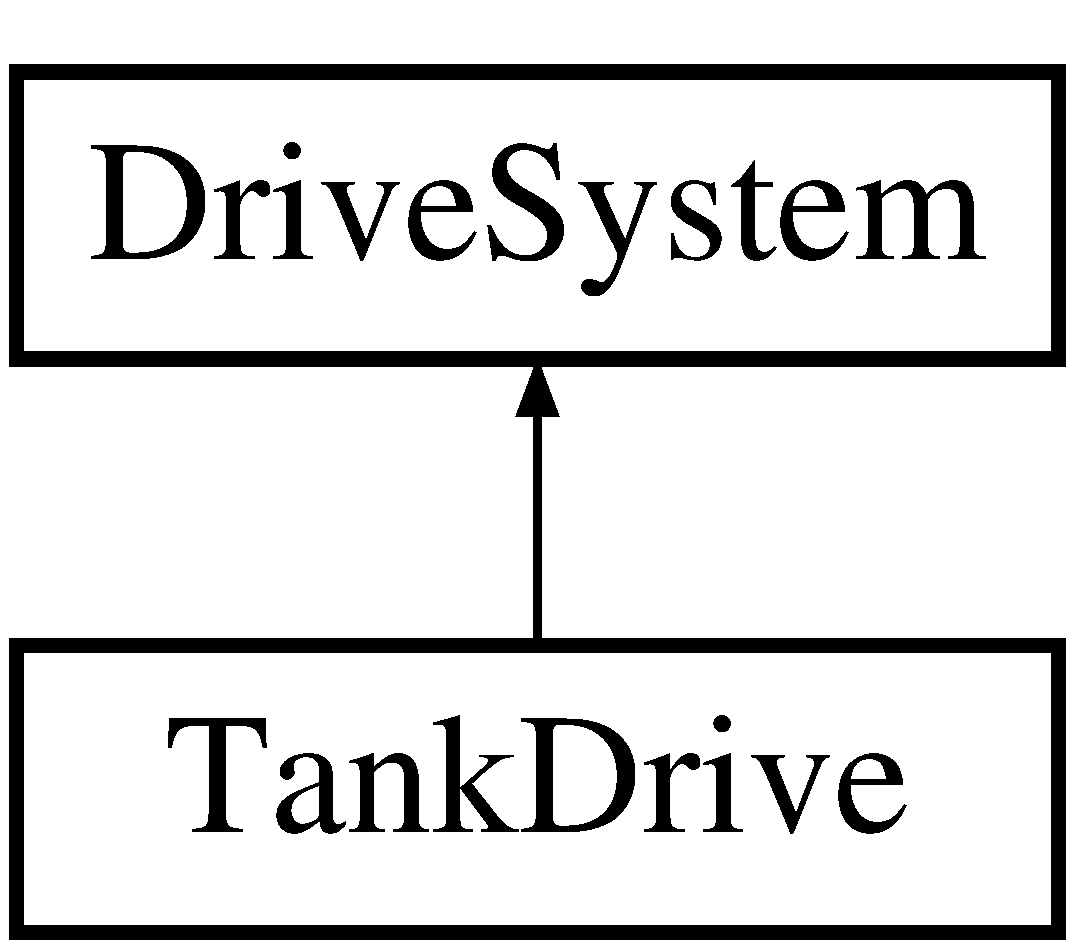
\includegraphics[height=2.000000cm]{classDriveSystem}
\end{center}
\end{figure}
\subsection*{Public Member Functions}
\begin{DoxyCompactItemize}
\item 
\hyperlink{classDriveSystem_ae01dd44e98832cd3fd53d34e11d53daa}{Drive\-System} ()
\item 
virtual \hyperlink{classDriveSystem_ab571a24395df418db8721d1e75348c2a}{$\sim$\-Drive\-System} ()
\item 
void \hyperlink{classDriveSystem_add520db676d50658a45813bc4620ed28}{set\-Chassis\-Name} (std\-::string name)
\begin{DoxyCompactList}\small\item\em Set the chassis name to which this drive system belongs. \end{DoxyCompactList}\item 
std\-::string \hyperlink{classDriveSystem_ae7099ada003ded0f8e29f1394e41c88a}{get\-Chassis\-Name} ()
\begin{DoxyCompactList}\small\item\em Get the name for the chassis to which this drive system belongs. \end{DoxyCompactList}\item 
void \hyperlink{classDriveSystem_a0fcba2555b44f81ba8a4f8eb07119a2d}{set\-Max\-Velocity} (\hyperlink{classMotorVelocity}{Motor\-Velocity} velocity)
\begin{DoxyCompactList}\small\item\em Set the maximum velocity at which this drive system can operate effectively. \end{DoxyCompactList}\item 
\hyperlink{classMotorVelocity}{Motor\-Velocity} \hyperlink{classDriveSystem_ac34dc1ce697223d25f978ba2ace3a164}{get\-Max\-Velocity} ()
\begin{DoxyCompactList}\small\item\em Get the maximum velocity at which this drive system can operate effectively. \end{DoxyCompactList}\item 
void \hyperlink{classDriveSystem_a4c2924e7b017844a0517e1a915761e0b}{set\-Max\-Acceleration} (\hyperlink{classMotorAcceleration}{Motor\-Acceleration} acceleration)
\begin{DoxyCompactList}\small\item\em Set the maximum acceleration at which this drive system can operate effectively. \end{DoxyCompactList}\item 
\hyperlink{classMotorAcceleration}{Motor\-Acceleration} \hyperlink{classDriveSystem_a6d675fc43ab54446f62d1abb9e888ac5}{get\-Max\-Acceleration} ()
\begin{DoxyCompactList}\small\item\em Get the maximum acceleration at which this drive system can operate effectively. \end{DoxyCompactList}\item 
void \hyperlink{classDriveSystem_a3db4b8e79e330dbf2a013cc8c7c462b5}{set\-Motor\-Rot\-Per\-Movement\-Foot} (double rotations)
\begin{DoxyCompactList}\small\item\em Set the number of motor rotations required to move the drive system one foot. \end{DoxyCompactList}\item 
double \hyperlink{classDriveSystem_a0ec467bebb7953e764e81435c6a75f2d}{get\-Motor\-Rot\-Per\-Movement\-Foot} ()
\begin{DoxyCompactList}\small\item\em Get the number of motor rotations required to move the drive system one foot. \end{DoxyCompactList}\item 
void \hyperlink{classDriveSystem_afc47457d594e21405383a680194c834c}{set\-Trajectory\-Iteration\-Period\-M\-S} (unsigned int period)
\begin{DoxyCompactList}\small\item\em Set the iteration period (in milliseconds) to be used for each trajectory point. \end{DoxyCompactList}\item 
unsigned int \hyperlink{classDriveSystem_a6e1dd3cebd19be585ccf2a9079230cfd}{get\-Trajectory\-Iteration\-Period\-M\-S} ()
\begin{DoxyCompactList}\small\item\em Get the iteration period (in milliseconds) to be used for each trajectory point. \end{DoxyCompactList}\item 
virtual void \hyperlink{classDriveSystem_af0f174a092b6b4a13ae589a1d72ff0c8}{move} (double distance\-Feet, \hyperlink{classChassisTurnRate}{Chassis\-Turn\-Rate} chassis\-Turn\-Rate, \hyperlink{classChassisVelocity}{Chassis\-Velocity} chassis\-Velocity\-Requested, \hyperlink{classChassisAcceleration}{Chassis\-Acceleration} chassis\-Acceleration\-Requested)
\begin{DoxyCompactList}\small\item\em A \char`\"{}filler\char`\"{} method in the base class to prevent link errors; redefined in derived classes. \end{DoxyCompactList}\end{DoxyCompactItemize}
\subsection*{Protected Attributes}
\begin{DoxyCompactItemize}
\item 
std\-::string \hyperlink{classDriveSystem_a9751d2041e38600dafc1d4575f0b7c2a}{chassis\-Name}
\item 
\hyperlink{classMotorVelocity}{Motor\-Velocity} \hyperlink{classDriveSystem_a3a9b75c1ae1147548d155a64432cedc4}{max\-Velocity}
\item 
\hyperlink{classMotorAcceleration}{Motor\-Acceleration} \hyperlink{classDriveSystem_a3f36b9c2b93fb6ed87cdb698a812087e}{max\-Acceleration}
\item 
double \hyperlink{classDriveSystem_acb0ea84b9cff42cd2b3619da7547ec06}{motor\-Rot\-Per\-Movement\-Foot}
\item 
unsigned int \hyperlink{classDriveSystem_a718e69f0338b27d50e79d698886aa744}{trajectory\-Iteration\-Period\-M\-S}
\end{DoxyCompactItemize}


\subsection{Detailed Description}
Base class for representing drive system objects. 

\subsection{Constructor \& Destructor Documentation}
\hypertarget{classDriveSystem_ae01dd44e98832cd3fd53d34e11d53daa}{\index{Drive\-System@{Drive\-System}!Drive\-System@{Drive\-System}}
\index{Drive\-System@{Drive\-System}!DriveSystem@{Drive\-System}}
\subsubsection[{Drive\-System}]{\setlength{\rightskip}{0pt plus 5cm}Drive\-System\-::\-Drive\-System (
\begin{DoxyParamCaption}
{}
\end{DoxyParamCaption}
)}}\label{classDriveSystem_ae01dd44e98832cd3fd53d34e11d53daa}
\hypertarget{classDriveSystem_ab571a24395df418db8721d1e75348c2a}{\index{Drive\-System@{Drive\-System}!$\sim$\-Drive\-System@{$\sim$\-Drive\-System}}
\index{$\sim$\-Drive\-System@{$\sim$\-Drive\-System}!DriveSystem@{Drive\-System}}
\subsubsection[{$\sim$\-Drive\-System}]{\setlength{\rightskip}{0pt plus 5cm}Drive\-System\-::$\sim$\-Drive\-System (
\begin{DoxyParamCaption}
{}
\end{DoxyParamCaption}
)\hspace{0.3cm}{\ttfamily [virtual]}}}\label{classDriveSystem_ab571a24395df418db8721d1e75348c2a}


\subsection{Member Function Documentation}
\hypertarget{classDriveSystem_ae7099ada003ded0f8e29f1394e41c88a}{\index{Drive\-System@{Drive\-System}!get\-Chassis\-Name@{get\-Chassis\-Name}}
\index{get\-Chassis\-Name@{get\-Chassis\-Name}!DriveSystem@{Drive\-System}}
\subsubsection[{get\-Chassis\-Name}]{\setlength{\rightskip}{0pt plus 5cm}std\-::string Drive\-System\-::get\-Chassis\-Name (
\begin{DoxyParamCaption}
{}
\end{DoxyParamCaption}
)}}\label{classDriveSystem_ae7099ada003ded0f8e29f1394e41c88a}


Get the name for the chassis to which this drive system belongs. 

\begin{DoxyReturn}{Returns}
std\-::string chassis\-Name of the chassis to which this drive system belongs 
\end{DoxyReturn}
\hypertarget{classDriveSystem_a6d675fc43ab54446f62d1abb9e888ac5}{\index{Drive\-System@{Drive\-System}!get\-Max\-Acceleration@{get\-Max\-Acceleration}}
\index{get\-Max\-Acceleration@{get\-Max\-Acceleration}!DriveSystem@{Drive\-System}}
\subsubsection[{get\-Max\-Acceleration}]{\setlength{\rightskip}{0pt plus 5cm}{\bf Motor\-Acceleration} Drive\-System\-::get\-Max\-Acceleration (
\begin{DoxyParamCaption}
{}
\end{DoxyParamCaption}
)}}\label{classDriveSystem_a6d675fc43ab54446f62d1abb9e888ac5}


Get the maximum acceleration at which this drive system can operate effectively. 

\begin{DoxyReturn}{Returns}
\hyperlink{classMotorAcceleration}{Motor\-Acceleration} acceleration at which this drive system can operate effectively 
\end{DoxyReturn}
\hypertarget{classDriveSystem_ac34dc1ce697223d25f978ba2ace3a164}{\index{Drive\-System@{Drive\-System}!get\-Max\-Velocity@{get\-Max\-Velocity}}
\index{get\-Max\-Velocity@{get\-Max\-Velocity}!DriveSystem@{Drive\-System}}
\subsubsection[{get\-Max\-Velocity}]{\setlength{\rightskip}{0pt plus 5cm}{\bf Motor\-Velocity} Drive\-System\-::get\-Max\-Velocity (
\begin{DoxyParamCaption}
{}
\end{DoxyParamCaption}
)}}\label{classDriveSystem_ac34dc1ce697223d25f978ba2ace3a164}


Get the maximum velocity at which this drive system can operate effectively. 

\begin{DoxyReturn}{Returns}
\hyperlink{classMotorVelocity}{Motor\-Velocity} velocity at which this drive system can operate effectively 
\end{DoxyReturn}
\hypertarget{classDriveSystem_a0ec467bebb7953e764e81435c6a75f2d}{\index{Drive\-System@{Drive\-System}!get\-Motor\-Rot\-Per\-Movement\-Foot@{get\-Motor\-Rot\-Per\-Movement\-Foot}}
\index{get\-Motor\-Rot\-Per\-Movement\-Foot@{get\-Motor\-Rot\-Per\-Movement\-Foot}!DriveSystem@{Drive\-System}}
\subsubsection[{get\-Motor\-Rot\-Per\-Movement\-Foot}]{\setlength{\rightskip}{0pt plus 5cm}double Drive\-System\-::get\-Motor\-Rot\-Per\-Movement\-Foot (
\begin{DoxyParamCaption}
{}
\end{DoxyParamCaption}
)}}\label{classDriveSystem_a0ec467bebb7953e764e81435c6a75f2d}


Get the number of motor rotations required to move the drive system one foot. 

\begin{DoxyReturn}{Returns}
double rotations of the motor per foot of movement 
\end{DoxyReturn}
\hypertarget{classDriveSystem_a6e1dd3cebd19be585ccf2a9079230cfd}{\index{Drive\-System@{Drive\-System}!get\-Trajectory\-Iteration\-Period\-M\-S@{get\-Trajectory\-Iteration\-Period\-M\-S}}
\index{get\-Trajectory\-Iteration\-Period\-M\-S@{get\-Trajectory\-Iteration\-Period\-M\-S}!DriveSystem@{Drive\-System}}
\subsubsection[{get\-Trajectory\-Iteration\-Period\-M\-S}]{\setlength{\rightskip}{0pt plus 5cm}unsigned int Drive\-System\-::get\-Trajectory\-Iteration\-Period\-M\-S (
\begin{DoxyParamCaption}
{}
\end{DoxyParamCaption}
)}}\label{classDriveSystem_a6e1dd3cebd19be585ccf2a9079230cfd}


Get the iteration period (in milliseconds) to be used for each trajectory point. 

\begin{DoxyReturn}{Returns}
unsigned int period for trajectory points in milliseconds 
\end{DoxyReturn}
\hypertarget{classDriveSystem_af0f174a092b6b4a13ae589a1d72ff0c8}{\index{Drive\-System@{Drive\-System}!move@{move}}
\index{move@{move}!DriveSystem@{Drive\-System}}
\subsubsection[{move}]{\setlength{\rightskip}{0pt plus 5cm}void Drive\-System\-::move (
\begin{DoxyParamCaption}
\item[{double}]{distance\-Feet, }
\item[{{\bf Chassis\-Turn\-Rate}}]{chassis\-Turn\-Rate, }
\item[{{\bf Chassis\-Velocity}}]{chassis\-Velocity\-Requested, }
\item[{{\bf Chassis\-Acceleration}}]{chassis\-Acceleration\-Requested}
\end{DoxyParamCaption}
)\hspace{0.3cm}{\ttfamily [virtual]}}}\label{classDriveSystem_af0f174a092b6b4a13ae589a1d72ff0c8}


A \char`\"{}filler\char`\"{} method in the base class to prevent link errors; redefined in derived classes. 


\begin{DoxyParams}{Parameters}
{\em distance\-Feet} & \\
\hline
{\em chassis\-Turn\-Rate} & \\
\hline
{\em chassis\-Velocity\-Requested} & \\
\hline
{\em chassis\-Acceleration\-Requested} & \\
\hline
\end{DoxyParams}


Reimplemented in \hyperlink{classTankDrive_ab4f103bfd11ab28c18ef292a505c454e}{Tank\-Drive}.

\hypertarget{classDriveSystem_add520db676d50658a45813bc4620ed28}{\index{Drive\-System@{Drive\-System}!set\-Chassis\-Name@{set\-Chassis\-Name}}
\index{set\-Chassis\-Name@{set\-Chassis\-Name}!DriveSystem@{Drive\-System}}
\subsubsection[{set\-Chassis\-Name}]{\setlength{\rightskip}{0pt plus 5cm}void Drive\-System\-::set\-Chassis\-Name (
\begin{DoxyParamCaption}
\item[{std\-::string}]{name}
\end{DoxyParamCaption}
)}}\label{classDriveSystem_add520db676d50658a45813bc4620ed28}


Set the chassis name to which this drive system belongs. 


\begin{DoxyParams}[1]{Parameters}
\mbox{\tt in}  & {\em std\-::string} & name that matches the chassis name to which this drive system belongs \\
\hline
\end{DoxyParams}
\hypertarget{classDriveSystem_a4c2924e7b017844a0517e1a915761e0b}{\index{Drive\-System@{Drive\-System}!set\-Max\-Acceleration@{set\-Max\-Acceleration}}
\index{set\-Max\-Acceleration@{set\-Max\-Acceleration}!DriveSystem@{Drive\-System}}
\subsubsection[{set\-Max\-Acceleration}]{\setlength{\rightskip}{0pt plus 5cm}void Drive\-System\-::set\-Max\-Acceleration (
\begin{DoxyParamCaption}
\item[{{\bf Motor\-Acceleration}}]{acceleration}
\end{DoxyParamCaption}
)}}\label{classDriveSystem_a4c2924e7b017844a0517e1a915761e0b}


Set the maximum acceleration at which this drive system can operate effectively. 


\begin{DoxyParams}[1]{Parameters}
\mbox{\tt in}  & {\em \hyperlink{classMotorAcceleration}{Motor\-Acceleration}} & acceleration at which this drive system can operate effectively \\
\hline
\end{DoxyParams}
\hypertarget{classDriveSystem_a0fcba2555b44f81ba8a4f8eb07119a2d}{\index{Drive\-System@{Drive\-System}!set\-Max\-Velocity@{set\-Max\-Velocity}}
\index{set\-Max\-Velocity@{set\-Max\-Velocity}!DriveSystem@{Drive\-System}}
\subsubsection[{set\-Max\-Velocity}]{\setlength{\rightskip}{0pt plus 5cm}void Drive\-System\-::set\-Max\-Velocity (
\begin{DoxyParamCaption}
\item[{{\bf Motor\-Velocity}}]{velocity}
\end{DoxyParamCaption}
)}}\label{classDriveSystem_a0fcba2555b44f81ba8a4f8eb07119a2d}


Set the maximum velocity at which this drive system can operate effectively. 


\begin{DoxyParams}[1]{Parameters}
\mbox{\tt in}  & {\em \hyperlink{classMotorVelocity}{Motor\-Velocity}} & velocity at which this drive system can operate effectively \\
\hline
\end{DoxyParams}
\hypertarget{classDriveSystem_a3db4b8e79e330dbf2a013cc8c7c462b5}{\index{Drive\-System@{Drive\-System}!set\-Motor\-Rot\-Per\-Movement\-Foot@{set\-Motor\-Rot\-Per\-Movement\-Foot}}
\index{set\-Motor\-Rot\-Per\-Movement\-Foot@{set\-Motor\-Rot\-Per\-Movement\-Foot}!DriveSystem@{Drive\-System}}
\subsubsection[{set\-Motor\-Rot\-Per\-Movement\-Foot}]{\setlength{\rightskip}{0pt plus 5cm}void Drive\-System\-::set\-Motor\-Rot\-Per\-Movement\-Foot (
\begin{DoxyParamCaption}
\item[{double}]{rotations}
\end{DoxyParamCaption}
)}}\label{classDriveSystem_a3db4b8e79e330dbf2a013cc8c7c462b5}


Set the number of motor rotations required to move the drive system one foot. 


\begin{DoxyParams}[1]{Parameters}
\mbox{\tt in}  & {\em double} & rotations of the motor per foot of movement \\
\hline
\end{DoxyParams}
\hypertarget{classDriveSystem_afc47457d594e21405383a680194c834c}{\index{Drive\-System@{Drive\-System}!set\-Trajectory\-Iteration\-Period\-M\-S@{set\-Trajectory\-Iteration\-Period\-M\-S}}
\index{set\-Trajectory\-Iteration\-Period\-M\-S@{set\-Trajectory\-Iteration\-Period\-M\-S}!DriveSystem@{Drive\-System}}
\subsubsection[{set\-Trajectory\-Iteration\-Period\-M\-S}]{\setlength{\rightskip}{0pt plus 5cm}void Drive\-System\-::set\-Trajectory\-Iteration\-Period\-M\-S (
\begin{DoxyParamCaption}
\item[{unsigned int}]{period}
\end{DoxyParamCaption}
)}}\label{classDriveSystem_afc47457d594e21405383a680194c834c}


Set the iteration period (in milliseconds) to be used for each trajectory point. 


\begin{DoxyParams}[1]{Parameters}
\mbox{\tt in}  & {\em unsigned} & int period for trajectory points in milliseconds \\
\hline
\end{DoxyParams}


\subsection{Member Data Documentation}
\hypertarget{classDriveSystem_a9751d2041e38600dafc1d4575f0b7c2a}{\index{Drive\-System@{Drive\-System}!chassis\-Name@{chassis\-Name}}
\index{chassis\-Name@{chassis\-Name}!DriveSystem@{Drive\-System}}
\subsubsection[{chassis\-Name}]{\setlength{\rightskip}{0pt plus 5cm}std\-::string Drive\-System\-::chassis\-Name\hspace{0.3cm}{\ttfamily [protected]}}}\label{classDriveSystem_a9751d2041e38600dafc1d4575f0b7c2a}
\hypertarget{classDriveSystem_a3f36b9c2b93fb6ed87cdb698a812087e}{\index{Drive\-System@{Drive\-System}!max\-Acceleration@{max\-Acceleration}}
\index{max\-Acceleration@{max\-Acceleration}!DriveSystem@{Drive\-System}}
\subsubsection[{max\-Acceleration}]{\setlength{\rightskip}{0pt plus 5cm}{\bf Motor\-Acceleration} Drive\-System\-::max\-Acceleration\hspace{0.3cm}{\ttfamily [protected]}}}\label{classDriveSystem_a3f36b9c2b93fb6ed87cdb698a812087e}
\hypertarget{classDriveSystem_a3a9b75c1ae1147548d155a64432cedc4}{\index{Drive\-System@{Drive\-System}!max\-Velocity@{max\-Velocity}}
\index{max\-Velocity@{max\-Velocity}!DriveSystem@{Drive\-System}}
\subsubsection[{max\-Velocity}]{\setlength{\rightskip}{0pt plus 5cm}{\bf Motor\-Velocity} Drive\-System\-::max\-Velocity\hspace{0.3cm}{\ttfamily [protected]}}}\label{classDriveSystem_a3a9b75c1ae1147548d155a64432cedc4}
\hypertarget{classDriveSystem_acb0ea84b9cff42cd2b3619da7547ec06}{\index{Drive\-System@{Drive\-System}!motor\-Rot\-Per\-Movement\-Foot@{motor\-Rot\-Per\-Movement\-Foot}}
\index{motor\-Rot\-Per\-Movement\-Foot@{motor\-Rot\-Per\-Movement\-Foot}!DriveSystem@{Drive\-System}}
\subsubsection[{motor\-Rot\-Per\-Movement\-Foot}]{\setlength{\rightskip}{0pt plus 5cm}double Drive\-System\-::motor\-Rot\-Per\-Movement\-Foot\hspace{0.3cm}{\ttfamily [protected]}}}\label{classDriveSystem_acb0ea84b9cff42cd2b3619da7547ec06}
\hypertarget{classDriveSystem_a718e69f0338b27d50e79d698886aa744}{\index{Drive\-System@{Drive\-System}!trajectory\-Iteration\-Period\-M\-S@{trajectory\-Iteration\-Period\-M\-S}}
\index{trajectory\-Iteration\-Period\-M\-S@{trajectory\-Iteration\-Period\-M\-S}!DriveSystem@{Drive\-System}}
\subsubsection[{trajectory\-Iteration\-Period\-M\-S}]{\setlength{\rightskip}{0pt plus 5cm}unsigned int Drive\-System\-::trajectory\-Iteration\-Period\-M\-S\hspace{0.3cm}{\ttfamily [protected]}}}\label{classDriveSystem_a718e69f0338b27d50e79d698886aa744}


The documentation for this class was generated from the following files\-:\begin{DoxyCompactItemize}
\item 
framework/\hyperlink{DriveSystem_8hpp}{Drive\-System.\-hpp}\item 
framework/\hyperlink{DriveSystem_8cpp}{Drive\-System.\-cpp}\end{DoxyCompactItemize}

\hypertarget{classMotorAcceleration}{\section{Motor\-Acceleration Class Reference}
\label{classMotorAcceleration}\index{Motor\-Acceleration@{Motor\-Acceleration}}
}


A class to provide a strict type for specifying motor acceleration.  




{\ttfamily \#include $<$Motor\-Acceleration.\-hpp$>$}

\subsection*{Public Member Functions}
\begin{DoxyCompactItemize}
\item 
\hyperlink{classMotorAcceleration_a72f063dc64724f540d7decff01a23f6f}{Motor\-Acceleration} ()
\item 
virtual \hyperlink{classMotorAcceleration_a0726b77fa1f8d306f7396e19a8cd4f45}{$\sim$\-Motor\-Acceleration} ()
\item 
void \hyperlink{classMotorAcceleration_afab1d3a188fff9779b581dcdb82310cb}{set\-Rotations\-Per\-Minute\-Per\-Second} (const double rate)
\begin{DoxyCompactList}\small\item\em Set a motor acceleration value in Rotations per Minute per second. \end{DoxyCompactList}\item 
void \hyperlink{classMotorAcceleration_a2d02913363b7ccbec7dea4d42bfed268}{set\-From\-Chassis\-Acceleration\-By\-Rot\-Per\-Movement\-Foot} (\hyperlink{classChassisAcceleration}{Chassis\-Acceleration} chassis\-Acceleration, double rot\-Per\-Movement\-Foot)
\begin{DoxyCompactList}\small\item\em Set a motor acceleration value from a chassis acceleration object. \end{DoxyCompactList}\item 
double \hyperlink{classMotorAcceleration_a51cc0b4db4e977b2076d23e77608e4aa}{get\-Rotations\-Per\-Minute\-Per\-Second} ()
\begin{DoxyCompactList}\small\item\em Get a motor acceleration value in Rotations per Minute per second. \end{DoxyCompactList}\end{DoxyCompactItemize}
\subsection*{Private Attributes}
\begin{DoxyCompactItemize}
\item 
double \hyperlink{classMotorAcceleration_ae9c0873fe1fb6752b9584ace95e11635}{accel\-As\-Rotations\-Per\-Minute\-Per\-Second}
\end{DoxyCompactItemize}


\subsection{Detailed Description}
A class to provide a strict type for specifying motor acceleration. 

\subsection{Constructor \& Destructor Documentation}
\hypertarget{classMotorAcceleration_a72f063dc64724f540d7decff01a23f6f}{\index{Motor\-Acceleration@{Motor\-Acceleration}!Motor\-Acceleration@{Motor\-Acceleration}}
\index{Motor\-Acceleration@{Motor\-Acceleration}!MotorAcceleration@{Motor\-Acceleration}}
\subsubsection[{Motor\-Acceleration}]{\setlength{\rightskip}{0pt plus 5cm}Motor\-Acceleration\-::\-Motor\-Acceleration (
\begin{DoxyParamCaption}
{}
\end{DoxyParamCaption}
)}}\label{classMotorAcceleration_a72f063dc64724f540d7decff01a23f6f}
\hypertarget{classMotorAcceleration_a0726b77fa1f8d306f7396e19a8cd4f45}{\index{Motor\-Acceleration@{Motor\-Acceleration}!$\sim$\-Motor\-Acceleration@{$\sim$\-Motor\-Acceleration}}
\index{$\sim$\-Motor\-Acceleration@{$\sim$\-Motor\-Acceleration}!MotorAcceleration@{Motor\-Acceleration}}
\subsubsection[{$\sim$\-Motor\-Acceleration}]{\setlength{\rightskip}{0pt plus 5cm}Motor\-Acceleration\-::$\sim$\-Motor\-Acceleration (
\begin{DoxyParamCaption}
{}
\end{DoxyParamCaption}
)\hspace{0.3cm}{\ttfamily [virtual]}}}\label{classMotorAcceleration_a0726b77fa1f8d306f7396e19a8cd4f45}


\subsection{Member Function Documentation}
\hypertarget{classMotorAcceleration_a51cc0b4db4e977b2076d23e77608e4aa}{\index{Motor\-Acceleration@{Motor\-Acceleration}!get\-Rotations\-Per\-Minute\-Per\-Second@{get\-Rotations\-Per\-Minute\-Per\-Second}}
\index{get\-Rotations\-Per\-Minute\-Per\-Second@{get\-Rotations\-Per\-Minute\-Per\-Second}!MotorAcceleration@{Motor\-Acceleration}}
\subsubsection[{get\-Rotations\-Per\-Minute\-Per\-Second}]{\setlength{\rightskip}{0pt plus 5cm}double Motor\-Acceleration\-::get\-Rotations\-Per\-Minute\-Per\-Second (
\begin{DoxyParamCaption}
{}
\end{DoxyParamCaption}
)}}\label{classMotorAcceleration_a51cc0b4db4e977b2076d23e77608e4aa}


Get a motor acceleration value in Rotations per Minute per second. 

\begin{DoxyReturn}{Returns}
a double representing the motor acceleration value 
\end{DoxyReturn}
\hypertarget{classMotorAcceleration_a2d02913363b7ccbec7dea4d42bfed268}{\index{Motor\-Acceleration@{Motor\-Acceleration}!set\-From\-Chassis\-Acceleration\-By\-Rot\-Per\-Movement\-Foot@{set\-From\-Chassis\-Acceleration\-By\-Rot\-Per\-Movement\-Foot}}
\index{set\-From\-Chassis\-Acceleration\-By\-Rot\-Per\-Movement\-Foot@{set\-From\-Chassis\-Acceleration\-By\-Rot\-Per\-Movement\-Foot}!MotorAcceleration@{Motor\-Acceleration}}
\subsubsection[{set\-From\-Chassis\-Acceleration\-By\-Rot\-Per\-Movement\-Foot}]{\setlength{\rightskip}{0pt plus 5cm}void Motor\-Acceleration\-::set\-From\-Chassis\-Acceleration\-By\-Rot\-Per\-Movement\-Foot (
\begin{DoxyParamCaption}
\item[{{\bf Chassis\-Acceleration}}]{chassis\-Acceleration, }
\item[{double}]{rot\-Per\-Movement\-Foot}
\end{DoxyParamCaption}
)}}\label{classMotorAcceleration_a2d02913363b7ccbec7dea4d42bfed268}


Set a motor acceleration value from a chassis acceleration object. 


\begin{DoxyParams}[1]{Parameters}
\mbox{\tt in}  & {\em \hyperlink{classChassisAcceleration}{Chassis\-Acceleration}} & chassis\-Acceleration object \\
\hline
\mbox{\tt in}  & {\em double} & rot\-Per\-Movement\-Foot specifying the rotations per movement foot \\
\hline
\end{DoxyParams}
\hypertarget{classMotorAcceleration_afab1d3a188fff9779b581dcdb82310cb}{\index{Motor\-Acceleration@{Motor\-Acceleration}!set\-Rotations\-Per\-Minute\-Per\-Second@{set\-Rotations\-Per\-Minute\-Per\-Second}}
\index{set\-Rotations\-Per\-Minute\-Per\-Second@{set\-Rotations\-Per\-Minute\-Per\-Second}!MotorAcceleration@{Motor\-Acceleration}}
\subsubsection[{set\-Rotations\-Per\-Minute\-Per\-Second}]{\setlength{\rightskip}{0pt plus 5cm}void Motor\-Acceleration\-::set\-Rotations\-Per\-Minute\-Per\-Second (
\begin{DoxyParamCaption}
\item[{const double}]{rate}
\end{DoxyParamCaption}
)}}\label{classMotorAcceleration_afab1d3a188fff9779b581dcdb82310cb}


Set a motor acceleration value in Rotations per Minute per second. 


\begin{DoxyParams}[1]{Parameters}
\mbox{\tt in}  & {\em double} & rate to set as the acceleration value \\
\hline
\end{DoxyParams}


\subsection{Member Data Documentation}
\hypertarget{classMotorAcceleration_ae9c0873fe1fb6752b9584ace95e11635}{\index{Motor\-Acceleration@{Motor\-Acceleration}!accel\-As\-Rotations\-Per\-Minute\-Per\-Second@{accel\-As\-Rotations\-Per\-Minute\-Per\-Second}}
\index{accel\-As\-Rotations\-Per\-Minute\-Per\-Second@{accel\-As\-Rotations\-Per\-Minute\-Per\-Second}!MotorAcceleration@{Motor\-Acceleration}}
\subsubsection[{accel\-As\-Rotations\-Per\-Minute\-Per\-Second}]{\setlength{\rightskip}{0pt plus 5cm}double Motor\-Acceleration\-::accel\-As\-Rotations\-Per\-Minute\-Per\-Second\hspace{0.3cm}{\ttfamily [private]}}}\label{classMotorAcceleration_ae9c0873fe1fb6752b9584ace95e11635}


The documentation for this class was generated from the following files\-:\begin{DoxyCompactItemize}
\item 
framework/\hyperlink{MotorAcceleration_8hpp}{Motor\-Acceleration.\-hpp}\item 
framework/\hyperlink{MotorAcceleration_8cpp}{Motor\-Acceleration.\-cpp}\end{DoxyCompactItemize}

\hypertarget{classMotorPosition}{\section{Motor\-Position Class Reference}
\label{classMotorPosition}\index{Motor\-Position@{Motor\-Position}}
}


Creates a defined type for a position based on a motor encoder.  




{\ttfamily \#include $<$Motor\-Position.\-hpp$>$}

\subsection*{Public Member Functions}
\begin{DoxyCompactItemize}
\item 
\hyperlink{classMotorPosition_aff0b57531330258354815c98c21ccf22}{Motor\-Position} ()
\item 
virtual \hyperlink{classMotorPosition_a63f9a5f064dedeee8d54c19a07e3afd9}{$\sim$\-Motor\-Position} ()
\item 
void \hyperlink{classMotorPosition_aafd35469ff1364e2d7db6704c79af9b8}{set\-Rotations} (const double count)
\begin{DoxyCompactList}\small\item\em Set the motor position using a floating point (double) rotation count. \end{DoxyCompactList}\item 
void \hyperlink{classMotorPosition_a9b0f13dd755deb8bda8069b7c5eda11e}{set\-From\-Distance\-Feet\-By\-Rot\-Per\-Movement\-Foot} (const double distance\-Feet, const double rot\-Per\-Movement\-Foot)
\begin{DoxyCompactList}\small\item\em Convert a linear distance measure in feet to motor rotations using conversion factor. \end{DoxyCompactList}\item 
double \hyperlink{classMotorPosition_aff33869a933accaca983110601151ddf}{get\-Rotations} ()
\begin{DoxyCompactList}\small\item\em Return the motor position as a floating point (double) rotation count. \end{DoxyCompactList}\item 
\hyperlink{classMotorPosition}{Motor\-Position} \hyperlink{classMotorPosition_a32b180c8c51be1a15c46ecc3e216325f}{operator-\/} (const \hyperlink{classMotorPosition}{Motor\-Position} \&mp)
\begin{DoxyCompactList}\small\item\em Minus (-\/) operator to allow subtraction between Motor\-Positions. \end{DoxyCompactList}\end{DoxyCompactItemize}
\subsection*{Private Attributes}
\begin{DoxyCompactItemize}
\item 
double \hyperlink{classMotorPosition_aa275f06359509a8e951fbde9e7b55a36}{rotation\-Count}
\end{DoxyCompactItemize}


\subsection{Detailed Description}
Creates a defined type for a position based on a motor encoder. 

\subsection{Constructor \& Destructor Documentation}
\hypertarget{classMotorPosition_aff0b57531330258354815c98c21ccf22}{\index{Motor\-Position@{Motor\-Position}!Motor\-Position@{Motor\-Position}}
\index{Motor\-Position@{Motor\-Position}!MotorPosition@{Motor\-Position}}
\subsubsection[{Motor\-Position}]{\setlength{\rightskip}{0pt plus 5cm}Motor\-Position\-::\-Motor\-Position (
\begin{DoxyParamCaption}
{}
\end{DoxyParamCaption}
)}}\label{classMotorPosition_aff0b57531330258354815c98c21ccf22}
\hypertarget{classMotorPosition_a63f9a5f064dedeee8d54c19a07e3afd9}{\index{Motor\-Position@{Motor\-Position}!$\sim$\-Motor\-Position@{$\sim$\-Motor\-Position}}
\index{$\sim$\-Motor\-Position@{$\sim$\-Motor\-Position}!MotorPosition@{Motor\-Position}}
\subsubsection[{$\sim$\-Motor\-Position}]{\setlength{\rightskip}{0pt plus 5cm}Motor\-Position\-::$\sim$\-Motor\-Position (
\begin{DoxyParamCaption}
{}
\end{DoxyParamCaption}
)\hspace{0.3cm}{\ttfamily [virtual]}}}\label{classMotorPosition_a63f9a5f064dedeee8d54c19a07e3afd9}


\subsection{Member Function Documentation}
\hypertarget{classMotorPosition_aff33869a933accaca983110601151ddf}{\index{Motor\-Position@{Motor\-Position}!get\-Rotations@{get\-Rotations}}
\index{get\-Rotations@{get\-Rotations}!MotorPosition@{Motor\-Position}}
\subsubsection[{get\-Rotations}]{\setlength{\rightskip}{0pt plus 5cm}double Motor\-Position\-::get\-Rotations (
\begin{DoxyParamCaption}
{}
\end{DoxyParamCaption}
)}}\label{classMotorPosition_aff33869a933accaca983110601151ddf}


Return the motor position as a floating point (double) rotation count. 

\begin{DoxyReturn}{Returns}
the current position as a motor encoder rotation count 
\end{DoxyReturn}
\hypertarget{classMotorPosition_a32b180c8c51be1a15c46ecc3e216325f}{\index{Motor\-Position@{Motor\-Position}!operator-\/@{operator-\/}}
\index{operator-\/@{operator-\/}!MotorPosition@{Motor\-Position}}
\subsubsection[{operator-\/}]{\setlength{\rightskip}{0pt plus 5cm}{\bf Motor\-Position} Motor\-Position\-::operator-\/ (
\begin{DoxyParamCaption}
\item[{const {\bf Motor\-Position} \&}]{mp}
\end{DoxyParamCaption}
)}}\label{classMotorPosition_a32b180c8c51be1a15c46ecc3e216325f}


Minus (-\/) operator to allow subtraction between Motor\-Positions. 


\begin{DoxyParams}[1]{Parameters}
\mbox{\tt in}  & {\em \hyperlink{classMotorPosition}{Motor\-Position}} & mp -\/ the right operand of the subtraction operator \\
\hline
\end{DoxyParams}
\begin{DoxyReturn}{Returns}
\hyperlink{classMotorPosition}{Motor\-Position} representing the difference between the two operands 
\end{DoxyReturn}
\hypertarget{classMotorPosition_a9b0f13dd755deb8bda8069b7c5eda11e}{\index{Motor\-Position@{Motor\-Position}!set\-From\-Distance\-Feet\-By\-Rot\-Per\-Movement\-Foot@{set\-From\-Distance\-Feet\-By\-Rot\-Per\-Movement\-Foot}}
\index{set\-From\-Distance\-Feet\-By\-Rot\-Per\-Movement\-Foot@{set\-From\-Distance\-Feet\-By\-Rot\-Per\-Movement\-Foot}!MotorPosition@{Motor\-Position}}
\subsubsection[{set\-From\-Distance\-Feet\-By\-Rot\-Per\-Movement\-Foot}]{\setlength{\rightskip}{0pt plus 5cm}void Motor\-Position\-::set\-From\-Distance\-Feet\-By\-Rot\-Per\-Movement\-Foot (
\begin{DoxyParamCaption}
\item[{const double}]{distance\-Feet, }
\item[{const double}]{rot\-Per\-Movement\-Foot}
\end{DoxyParamCaption}
)}}\label{classMotorPosition_a9b0f13dd755deb8bda8069b7c5eda11e}


Convert a linear distance measure in feet to motor rotations using conversion factor. 


\begin{DoxyParams}[1]{Parameters}
\mbox{\tt in}  & {\em double} & distance\-Feet -\/ the linear distance measure \\
\hline
\mbox{\tt in}  & {\em double} & rot\-Per\-Movement\-Foot -\/ the conversion factor from 1 linear foot to motor rotations \\
\hline
\end{DoxyParams}
\hypertarget{classMotorPosition_aafd35469ff1364e2d7db6704c79af9b8}{\index{Motor\-Position@{Motor\-Position}!set\-Rotations@{set\-Rotations}}
\index{set\-Rotations@{set\-Rotations}!MotorPosition@{Motor\-Position}}
\subsubsection[{set\-Rotations}]{\setlength{\rightskip}{0pt plus 5cm}void Motor\-Position\-::set\-Rotations (
\begin{DoxyParamCaption}
\item[{const double}]{count}
\end{DoxyParamCaption}
)}}\label{classMotorPosition_aafd35469ff1364e2d7db6704c79af9b8}


Set the motor position using a floating point (double) rotation count. 


\begin{DoxyParams}[1]{Parameters}
\mbox{\tt in}  & {\em a} & count value in a double \\
\hline
\end{DoxyParams}


\subsection{Member Data Documentation}
\hypertarget{classMotorPosition_aa275f06359509a8e951fbde9e7b55a36}{\index{Motor\-Position@{Motor\-Position}!rotation\-Count@{rotation\-Count}}
\index{rotation\-Count@{rotation\-Count}!MotorPosition@{Motor\-Position}}
\subsubsection[{rotation\-Count}]{\setlength{\rightskip}{0pt plus 5cm}double Motor\-Position\-::rotation\-Count\hspace{0.3cm}{\ttfamily [private]}}}\label{classMotorPosition_aa275f06359509a8e951fbde9e7b55a36}


The documentation for this class was generated from the following files\-:\begin{DoxyCompactItemize}
\item 
framework/\hyperlink{MotorPosition_8hpp}{Motor\-Position.\-hpp}\item 
framework/\hyperlink{MotorPosition_8cpp}{Motor\-Position.\-cpp}\end{DoxyCompactItemize}

\hypertarget{classMotorVelocity}{\section{Motor\-Velocity Class Reference}
\label{classMotorVelocity}\index{Motor\-Velocity@{Motor\-Velocity}}
}


The \hyperlink{classMotorVelocity}{Motor\-Velocity} class is a strict type for motor velocities.  




{\ttfamily \#include $<$Motor\-Velocity.\-hpp$>$}

\subsection*{Public Member Functions}
\begin{DoxyCompactItemize}
\item 
\hyperlink{classMotorVelocity_a710b857c335bdf69b986b23799b808f7}{Motor\-Velocity} ()
\item 
virtual \hyperlink{classMotorVelocity_af9a29b17b271b8b6c45c624a6764253e}{$\sim$\-Motor\-Velocity} ()
\item 
void \hyperlink{classMotorVelocity_a2ad99a1d1f49d767fa4eea224071d3a1}{set\-Rotations\-Per\-Minute} (const double rate)
\begin{DoxyCompactList}\small\item\em Set motor velocity in units of Rotations per Minute. \end{DoxyCompactList}\item 
void \hyperlink{classMotorVelocity_a6c5872379f7055a2d19635c68200dcc6}{set\-From\-Chassis\-Velocity\-By\-Rot\-Per\-Movement\-Foot} (\hyperlink{classChassisVelocity}{Chassis\-Velocity} chassis\-Velocity, double rot\-Per\-Movement\-Foot)
\begin{DoxyCompactList}\small\item\em Convert from a Chass\-Velocity to motor rotations by Rotations per Movement Foot. \end{DoxyCompactList}\item 
double \hyperlink{classMotorVelocity_a765517747b7fc90d5c0aee77c066a830}{get\-Rotations\-Per\-Minute} ()
\begin{DoxyCompactList}\small\item\em Get motor velocity in units of Rotations per Minute. \end{DoxyCompactList}\end{DoxyCompactItemize}
\subsection*{Private Attributes}
\begin{DoxyCompactItemize}
\item 
double \hyperlink{classMotorVelocity_a1814d196cb74a2a0c1df5ce494714aea}{vel\-As\-Rotations\-Per\-Minute}
\end{DoxyCompactItemize}


\subsection{Detailed Description}
The \hyperlink{classMotorVelocity}{Motor\-Velocity} class is a strict type for motor velocities. 

\subsection{Constructor \& Destructor Documentation}
\hypertarget{classMotorVelocity_a710b857c335bdf69b986b23799b808f7}{\index{Motor\-Velocity@{Motor\-Velocity}!Motor\-Velocity@{Motor\-Velocity}}
\index{Motor\-Velocity@{Motor\-Velocity}!MotorVelocity@{Motor\-Velocity}}
\subsubsection[{Motor\-Velocity}]{\setlength{\rightskip}{0pt plus 5cm}Motor\-Velocity\-::\-Motor\-Velocity (
\begin{DoxyParamCaption}
{}
\end{DoxyParamCaption}
)}}\label{classMotorVelocity_a710b857c335bdf69b986b23799b808f7}
\hypertarget{classMotorVelocity_af9a29b17b271b8b6c45c624a6764253e}{\index{Motor\-Velocity@{Motor\-Velocity}!$\sim$\-Motor\-Velocity@{$\sim$\-Motor\-Velocity}}
\index{$\sim$\-Motor\-Velocity@{$\sim$\-Motor\-Velocity}!MotorVelocity@{Motor\-Velocity}}
\subsubsection[{$\sim$\-Motor\-Velocity}]{\setlength{\rightskip}{0pt plus 5cm}Motor\-Velocity\-::$\sim$\-Motor\-Velocity (
\begin{DoxyParamCaption}
{}
\end{DoxyParamCaption}
)\hspace{0.3cm}{\ttfamily [virtual]}}}\label{classMotorVelocity_af9a29b17b271b8b6c45c624a6764253e}


\subsection{Member Function Documentation}
\hypertarget{classMotorVelocity_a765517747b7fc90d5c0aee77c066a830}{\index{Motor\-Velocity@{Motor\-Velocity}!get\-Rotations\-Per\-Minute@{get\-Rotations\-Per\-Minute}}
\index{get\-Rotations\-Per\-Minute@{get\-Rotations\-Per\-Minute}!MotorVelocity@{Motor\-Velocity}}
\subsubsection[{get\-Rotations\-Per\-Minute}]{\setlength{\rightskip}{0pt plus 5cm}double Motor\-Velocity\-::get\-Rotations\-Per\-Minute (
\begin{DoxyParamCaption}
{}
\end{DoxyParamCaption}
)}}\label{classMotorVelocity_a765517747b7fc90d5c0aee77c066a830}


Get motor velocity in units of Rotations per Minute. 

\begin{DoxyReturn}{Returns}
double representing a motor velocity 
\end{DoxyReturn}
\hypertarget{classMotorVelocity_a6c5872379f7055a2d19635c68200dcc6}{\index{Motor\-Velocity@{Motor\-Velocity}!set\-From\-Chassis\-Velocity\-By\-Rot\-Per\-Movement\-Foot@{set\-From\-Chassis\-Velocity\-By\-Rot\-Per\-Movement\-Foot}}
\index{set\-From\-Chassis\-Velocity\-By\-Rot\-Per\-Movement\-Foot@{set\-From\-Chassis\-Velocity\-By\-Rot\-Per\-Movement\-Foot}!MotorVelocity@{Motor\-Velocity}}
\subsubsection[{set\-From\-Chassis\-Velocity\-By\-Rot\-Per\-Movement\-Foot}]{\setlength{\rightskip}{0pt plus 5cm}void Motor\-Velocity\-::set\-From\-Chassis\-Velocity\-By\-Rot\-Per\-Movement\-Foot (
\begin{DoxyParamCaption}
\item[{{\bf Chassis\-Velocity}}]{chassis\-Velocity, }
\item[{double}]{rot\-Per\-Movement\-Foot}
\end{DoxyParamCaption}
)}}\label{classMotorVelocity_a6c5872379f7055a2d19635c68200dcc6}


Convert from a Chass\-Velocity to motor rotations by Rotations per Movement Foot. 


\begin{DoxyParams}[1]{Parameters}
\mbox{\tt in}  & {\em \hyperlink{classChassisVelocity}{Chassis\-Velocity}} & chassis\-Velocity specifies a linear physical velocity \\
\hline
\mbox{\tt in}  & {\em double} & rot\-Per\-Movement\-Foot is the conversion factor from movement feet to rotations \\
\hline
\end{DoxyParams}
\hypertarget{classMotorVelocity_a2ad99a1d1f49d767fa4eea224071d3a1}{\index{Motor\-Velocity@{Motor\-Velocity}!set\-Rotations\-Per\-Minute@{set\-Rotations\-Per\-Minute}}
\index{set\-Rotations\-Per\-Minute@{set\-Rotations\-Per\-Minute}!MotorVelocity@{Motor\-Velocity}}
\subsubsection[{set\-Rotations\-Per\-Minute}]{\setlength{\rightskip}{0pt plus 5cm}void Motor\-Velocity\-::set\-Rotations\-Per\-Minute (
\begin{DoxyParamCaption}
\item[{const double}]{rate}
\end{DoxyParamCaption}
)}}\label{classMotorVelocity_a2ad99a1d1f49d767fa4eea224071d3a1}


Set motor velocity in units of Rotations per Minute. 


\begin{DoxyParams}[1]{Parameters}
\mbox{\tt in}  & {\em double} & rate representing a motor velocity \\
\hline
\end{DoxyParams}


\subsection{Member Data Documentation}
\hypertarget{classMotorVelocity_a1814d196cb74a2a0c1df5ce494714aea}{\index{Motor\-Velocity@{Motor\-Velocity}!vel\-As\-Rotations\-Per\-Minute@{vel\-As\-Rotations\-Per\-Minute}}
\index{vel\-As\-Rotations\-Per\-Minute@{vel\-As\-Rotations\-Per\-Minute}!MotorVelocity@{Motor\-Velocity}}
\subsubsection[{vel\-As\-Rotations\-Per\-Minute}]{\setlength{\rightskip}{0pt plus 5cm}double Motor\-Velocity\-::vel\-As\-Rotations\-Per\-Minute\hspace{0.3cm}{\ttfamily [private]}}}\label{classMotorVelocity_a1814d196cb74a2a0c1df5ce494714aea}


The documentation for this class was generated from the following files\-:\begin{DoxyCompactItemize}
\item 
framework/\hyperlink{MotorVelocity_8hpp}{Motor\-Velocity.\-hpp}\item 
framework/\hyperlink{MotorVelocity_8cpp}{Motor\-Velocity.\-cpp}\end{DoxyCompactItemize}

\hypertarget{classPath}{\section{Path Class Reference}
\label{classPath}\index{Path@{Path}}
}


A motion path is a series of path points between two Way Points.  




{\ttfamily \#include $<$Path.\-hpp$>$}

\subsection*{Public Member Functions}
\begin{DoxyCompactItemize}
\item 
\hyperlink{classPath_af26cfab021ddf49af73da3b2beca85ac}{Path} ()
\item 
virtual \hyperlink{classPath_a141da9ff89c85e0ba410b5a73864c267}{$\sim$\-Path} ()
\item 
void \hyperlink{classPath_a8d5ea7007516aeda4a10c61d59051c6c}{add\-Path\-Point} (const \hyperlink{classPathPoint}{Path\-Point} \&path\-Point)
\begin{DoxyCompactList}\small\item\em Add a path point onto this path. \end{DoxyCompactList}\item 
bool \hyperlink{classPath_a05cef868b03ff1f01fd54bb2801b3af6}{get\-First\-Path\-Point} (\hyperlink{classPathPoint}{Path\-Point} \&path\-Point)
\begin{DoxyCompactList}\small\item\em Return the first path point in the path. \end{DoxyCompactList}\item 
bool \hyperlink{classPath_a9b6d6aa8279ff4c475ad03b471f8bf2d}{get\-Next\-Path\-Point} (\hyperlink{classPathPoint}{Path\-Point} \&path\-Point)
\begin{DoxyCompactList}\small\item\em Return the next path point on the path. \end{DoxyCompactList}\item 
unsigned int \hyperlink{classPath_aab30b48bfb68c8070cf4b70738f785d5}{size} ()
\begin{DoxyCompactList}\small\item\em Reports the number of path points in this path. \end{DoxyCompactList}\item 
void \hyperlink{classPath_acda7c567cd035d2f0a8661c53880bc4b}{show} ()
\begin{DoxyCompactList}\small\item\em Shows this motion path on the default output device. \end{DoxyCompactList}\end{DoxyCompactItemize}
\subsection*{Private Attributes}
\begin{DoxyCompactItemize}
\item 
std\-::vector$<$ \hyperlink{classPathPoint}{Path\-Point} $>$ \hyperlink{classPath_a48208f93e5010f15f33f487c4fc63b00}{path}
\item 
std\-::vector$<$ \hyperlink{classPathPoint}{Path\-Point} $>$\-::size\-\_\-type \hyperlink{classPath_a29c205bd85a584663cdb5b4e61d6a871}{next\-Path\-Point}
\end{DoxyCompactItemize}


\subsection{Detailed Description}
A motion path is a series of path points between two Way Points. 

\subsection{Constructor \& Destructor Documentation}
\hypertarget{classPath_af26cfab021ddf49af73da3b2beca85ac}{\index{Path@{Path}!Path@{Path}}
\index{Path@{Path}!Path@{Path}}
\subsubsection[{Path}]{\setlength{\rightskip}{0pt plus 5cm}Path\-::\-Path (
\begin{DoxyParamCaption}
{}
\end{DoxyParamCaption}
)}}\label{classPath_af26cfab021ddf49af73da3b2beca85ac}
\hypertarget{classPath_a141da9ff89c85e0ba410b5a73864c267}{\index{Path@{Path}!$\sim$\-Path@{$\sim$\-Path}}
\index{$\sim$\-Path@{$\sim$\-Path}!Path@{Path}}
\subsubsection[{$\sim$\-Path}]{\setlength{\rightskip}{0pt plus 5cm}Path\-::$\sim$\-Path (
\begin{DoxyParamCaption}
{}
\end{DoxyParamCaption}
)\hspace{0.3cm}{\ttfamily [virtual]}}}\label{classPath_a141da9ff89c85e0ba410b5a73864c267}


\subsection{Member Function Documentation}
\hypertarget{classPath_a8d5ea7007516aeda4a10c61d59051c6c}{\index{Path@{Path}!add\-Path\-Point@{add\-Path\-Point}}
\index{add\-Path\-Point@{add\-Path\-Point}!Path@{Path}}
\subsubsection[{add\-Path\-Point}]{\setlength{\rightskip}{0pt plus 5cm}void Path\-::add\-Path\-Point (
\begin{DoxyParamCaption}
\item[{const {\bf Path\-Point} \&}]{path\-Point}
\end{DoxyParamCaption}
)}}\label{classPath_a8d5ea7007516aeda4a10c61d59051c6c}


Add a path point onto this path. 


\begin{DoxyParams}[1]{Parameters}
\mbox{\tt in}  & {\em a} & \hyperlink{classPathPoint}{Path\-Point} path\-Point to add to the current path \\
\hline
\end{DoxyParams}
\hypertarget{classPath_a05cef868b03ff1f01fd54bb2801b3af6}{\index{Path@{Path}!get\-First\-Path\-Point@{get\-First\-Path\-Point}}
\index{get\-First\-Path\-Point@{get\-First\-Path\-Point}!Path@{Path}}
\subsubsection[{get\-First\-Path\-Point}]{\setlength{\rightskip}{0pt plus 5cm}bool Path\-::get\-First\-Path\-Point (
\begin{DoxyParamCaption}
\item[{{\bf Path\-Point} \&}]{path\-Point}
\end{DoxyParamCaption}
)}}\label{classPath_a05cef868b03ff1f01fd54bb2801b3af6}


Return the first path point in the path. 


\begin{DoxyParams}[1]{Parameters}
\mbox{\tt out}  & {\em \hyperlink{classPathPoint}{Path\-Point}} & set equal to the value of the first path point on the path \\
\hline
\end{DoxyParams}
\begin{DoxyReturn}{Returns}
bool indication of whether the requested point was on the path 
\end{DoxyReturn}
\hypertarget{classPath_a9b6d6aa8279ff4c475ad03b471f8bf2d}{\index{Path@{Path}!get\-Next\-Path\-Point@{get\-Next\-Path\-Point}}
\index{get\-Next\-Path\-Point@{get\-Next\-Path\-Point}!Path@{Path}}
\subsubsection[{get\-Next\-Path\-Point}]{\setlength{\rightskip}{0pt plus 5cm}bool Path\-::get\-Next\-Path\-Point (
\begin{DoxyParamCaption}
\item[{{\bf Path\-Point} \&}]{path\-Point}
\end{DoxyParamCaption}
)}}\label{classPath_a9b6d6aa8279ff4c475ad03b471f8bf2d}


Return the next path point on the path. 


\begin{DoxyParams}[1]{Parameters}
\mbox{\tt out}  & {\em \hyperlink{classPathPoint}{Path\-Point}} & set equal to the value of the next path point on the path \\
\hline
\end{DoxyParams}
\begin{DoxyReturn}{Returns}
bool indication of whether the requested point was on the path 
\end{DoxyReturn}
\hypertarget{classPath_acda7c567cd035d2f0a8661c53880bc4b}{\index{Path@{Path}!show@{show}}
\index{show@{show}!Path@{Path}}
\subsubsection[{show}]{\setlength{\rightskip}{0pt plus 5cm}void Path\-::show (
\begin{DoxyParamCaption}
{}
\end{DoxyParamCaption}
)}}\label{classPath_acda7c567cd035d2f0a8661c53880bc4b}


Shows this motion path on the default output device. 

\hypertarget{classPath_aab30b48bfb68c8070cf4b70738f785d5}{\index{Path@{Path}!size@{size}}
\index{size@{size}!Path@{Path}}
\subsubsection[{size}]{\setlength{\rightskip}{0pt plus 5cm}unsigned int Path\-::size (
\begin{DoxyParamCaption}
{}
\end{DoxyParamCaption}
)}}\label{classPath_aab30b48bfb68c8070cf4b70738f785d5}


Reports the number of path points in this path. 

\begin{DoxyReturn}{Returns}
int number of path points in path 
\end{DoxyReturn}


\subsection{Member Data Documentation}
\hypertarget{classPath_a29c205bd85a584663cdb5b4e61d6a871}{\index{Path@{Path}!next\-Path\-Point@{next\-Path\-Point}}
\index{next\-Path\-Point@{next\-Path\-Point}!Path@{Path}}
\subsubsection[{next\-Path\-Point}]{\setlength{\rightskip}{0pt plus 5cm}std\-::vector$<${\bf Path\-Point}$>$\-::size\-\_\-type Path\-::next\-Path\-Point\hspace{0.3cm}{\ttfamily [private]}}}\label{classPath_a29c205bd85a584663cdb5b4e61d6a871}
\hypertarget{classPath_a48208f93e5010f15f33f487c4fc63b00}{\index{Path@{Path}!path@{path}}
\index{path@{path}!Path@{Path}}
\subsubsection[{path}]{\setlength{\rightskip}{0pt plus 5cm}std\-::vector$<${\bf Path\-Point}$>$ Path\-::path\hspace{0.3cm}{\ttfamily [private]}}}\label{classPath_a48208f93e5010f15f33f487c4fc63b00}


The documentation for this class was generated from the following files\-:\begin{DoxyCompactItemize}
\item 
framework/\hyperlink{Path_8hpp}{Path.\-hpp}\item 
framework/\hyperlink{Path_8cpp}{Path.\-cpp}\end{DoxyCompactItemize}

\hypertarget{classPathPoint}{\section{Path\-Point Class Reference}
\label{classPathPoint}\index{Path\-Point@{Path\-Point}}
}


A motion path point has a maximum velocity and acceleration for motion from this point.  




{\ttfamily \#include $<$Path\-Point.\-hpp$>$}

Inheritance diagram for Path\-Point\-:\begin{figure}[H]
\begin{center}
\leavevmode
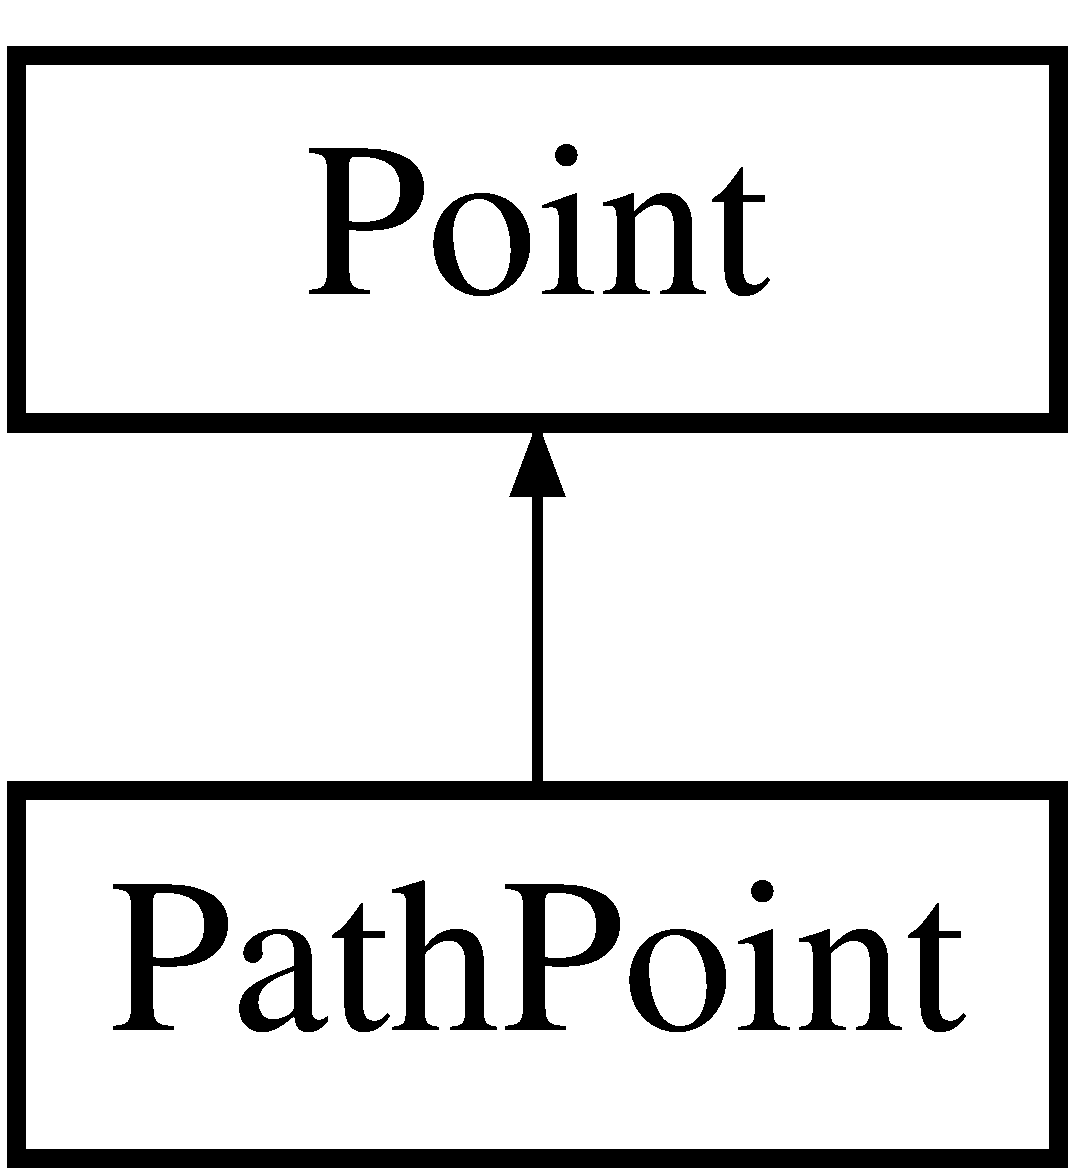
\includegraphics[height=2.000000cm]{classPathPoint}
\end{center}
\end{figure}
\subsection*{Public Member Functions}
\begin{DoxyCompactItemize}
\item 
\hyperlink{classPathPoint_a430ccd20bd3aca66d02e5762ada584cc}{Path\-Point} ()
\item 
virtual \hyperlink{classPathPoint_aa1186aedeb2f97861375d70c1f29baef}{$\sim$\-Path\-Point} ()
\item 
void \hyperlink{classPathPoint_af3cc40bbe896d63162c037a57476272f}{set\-Max\-Velocity} (const \hyperlink{classMotorVelocity}{Motor\-Velocity} \&max\-V)
\begin{DoxyCompactList}\small\item\em Set the maximum allowable velocity for this path point. \end{DoxyCompactList}\item 
\hyperlink{classMotorVelocity}{Motor\-Velocity} \hyperlink{classPathPoint_a7e32c122ba0bf4aefcc6684c2d30a69f}{get\-Max\-Velocity} ()
\begin{DoxyCompactList}\small\item\em Get the maximum allowable velocity for this path point. \end{DoxyCompactList}\item 
void \hyperlink{classPathPoint_a2d25367b2e4940967cb7cecda1549896}{set\-Max\-Acceleration} (const \hyperlink{classMotorAcceleration}{Motor\-Acceleration} \&max\-A)
\begin{DoxyCompactList}\small\item\em Set the maximum allowable acceleration for this path point. \end{DoxyCompactList}\item 
\hyperlink{classMotorAcceleration}{Motor\-Acceleration} \hyperlink{classPathPoint_a52f932842709dd6a9213e61252a9c273}{get\-Max\-Acceleration} ()
\begin{DoxyCompactList}\small\item\em Get the maximum allowable acceleration for this path point. \end{DoxyCompactList}\item 
void \hyperlink{classPathPoint_a9dec1d3f21b43b18a4b6daebb1c123de}{show} ()
\begin{DoxyCompactList}\small\item\em Show the details of the current path point. \end{DoxyCompactList}\end{DoxyCompactItemize}
\subsection*{Private Attributes}
\begin{DoxyCompactItemize}
\item 
\hyperlink{classMotorVelocity}{Motor\-Velocity} \hyperlink{classPathPoint_a1cc5f8871560f419edb85f24c6796613}{max\-Velocity}
\item 
\hyperlink{classMotorAcceleration}{Motor\-Acceleration} \hyperlink{classPathPoint_a70ea6c3945f895ebdfb34f8fa31b707e}{max\-Acceleration}
\end{DoxyCompactItemize}
\subsection*{Additional Inherited Members}


\subsection{Detailed Description}
A motion path point has a maximum velocity and acceleration for motion from this point. 

\subsection{Constructor \& Destructor Documentation}
\hypertarget{classPathPoint_a430ccd20bd3aca66d02e5762ada584cc}{\index{Path\-Point@{Path\-Point}!Path\-Point@{Path\-Point}}
\index{Path\-Point@{Path\-Point}!PathPoint@{Path\-Point}}
\subsubsection[{Path\-Point}]{\setlength{\rightskip}{0pt plus 5cm}Path\-Point\-::\-Path\-Point (
\begin{DoxyParamCaption}
{}
\end{DoxyParamCaption}
)}}\label{classPathPoint_a430ccd20bd3aca66d02e5762ada584cc}
\hypertarget{classPathPoint_aa1186aedeb2f97861375d70c1f29baef}{\index{Path\-Point@{Path\-Point}!$\sim$\-Path\-Point@{$\sim$\-Path\-Point}}
\index{$\sim$\-Path\-Point@{$\sim$\-Path\-Point}!PathPoint@{Path\-Point}}
\subsubsection[{$\sim$\-Path\-Point}]{\setlength{\rightskip}{0pt plus 5cm}Path\-Point\-::$\sim$\-Path\-Point (
\begin{DoxyParamCaption}
{}
\end{DoxyParamCaption}
)\hspace{0.3cm}{\ttfamily [virtual]}}}\label{classPathPoint_aa1186aedeb2f97861375d70c1f29baef}


\subsection{Member Function Documentation}
\hypertarget{classPathPoint_a52f932842709dd6a9213e61252a9c273}{\index{Path\-Point@{Path\-Point}!get\-Max\-Acceleration@{get\-Max\-Acceleration}}
\index{get\-Max\-Acceleration@{get\-Max\-Acceleration}!PathPoint@{Path\-Point}}
\subsubsection[{get\-Max\-Acceleration}]{\setlength{\rightskip}{0pt plus 5cm}{\bf Motor\-Acceleration} Path\-Point\-::get\-Max\-Acceleration (
\begin{DoxyParamCaption}
{}
\end{DoxyParamCaption}
)}}\label{classPathPoint_a52f932842709dd6a9213e61252a9c273}


Get the maximum allowable acceleration for this path point. 

\begin{DoxyReturn}{Returns}
a \hyperlink{classMotorAcceleration}{Motor\-Acceleration} value representing the maximum allowable acceleration 
\end{DoxyReturn}
\hypertarget{classPathPoint_a7e32c122ba0bf4aefcc6684c2d30a69f}{\index{Path\-Point@{Path\-Point}!get\-Max\-Velocity@{get\-Max\-Velocity}}
\index{get\-Max\-Velocity@{get\-Max\-Velocity}!PathPoint@{Path\-Point}}
\subsubsection[{get\-Max\-Velocity}]{\setlength{\rightskip}{0pt plus 5cm}{\bf Motor\-Velocity} Path\-Point\-::get\-Max\-Velocity (
\begin{DoxyParamCaption}
{}
\end{DoxyParamCaption}
)}}\label{classPathPoint_a7e32c122ba0bf4aefcc6684c2d30a69f}


Get the maximum allowable velocity for this path point. 

\begin{DoxyReturn}{Returns}
a \hyperlink{classMotorVelocity}{Motor\-Velocity} value representing the maximum allowable velocity 
\end{DoxyReturn}
\hypertarget{classPathPoint_a2d25367b2e4940967cb7cecda1549896}{\index{Path\-Point@{Path\-Point}!set\-Max\-Acceleration@{set\-Max\-Acceleration}}
\index{set\-Max\-Acceleration@{set\-Max\-Acceleration}!PathPoint@{Path\-Point}}
\subsubsection[{set\-Max\-Acceleration}]{\setlength{\rightskip}{0pt plus 5cm}void Path\-Point\-::set\-Max\-Acceleration (
\begin{DoxyParamCaption}
\item[{const {\bf Motor\-Acceleration} \&}]{max\-A}
\end{DoxyParamCaption}
)}}\label{classPathPoint_a2d25367b2e4940967cb7cecda1549896}


Set the maximum allowable acceleration for this path point. 


\begin{DoxyParams}[1]{Parameters}
\mbox{\tt in}  & {\em a} & \hyperlink{classMotorAcceleration}{Motor\-Acceleration} maximum allowable acceleration \\
\hline
\end{DoxyParams}
\hypertarget{classPathPoint_af3cc40bbe896d63162c037a57476272f}{\index{Path\-Point@{Path\-Point}!set\-Max\-Velocity@{set\-Max\-Velocity}}
\index{set\-Max\-Velocity@{set\-Max\-Velocity}!PathPoint@{Path\-Point}}
\subsubsection[{set\-Max\-Velocity}]{\setlength{\rightskip}{0pt plus 5cm}void Path\-Point\-::set\-Max\-Velocity (
\begin{DoxyParamCaption}
\item[{const {\bf Motor\-Velocity} \&}]{max\-V}
\end{DoxyParamCaption}
)}}\label{classPathPoint_af3cc40bbe896d63162c037a57476272f}


Set the maximum allowable velocity for this path point. 


\begin{DoxyParams}[1]{Parameters}
\mbox{\tt in}  & {\em a} & \hyperlink{classMotorVelocity}{Motor\-Velocity} maximum velocity \\
\hline
\end{DoxyParams}
\hypertarget{classPathPoint_a9dec1d3f21b43b18a4b6daebb1c123de}{\index{Path\-Point@{Path\-Point}!show@{show}}
\index{show@{show}!PathPoint@{Path\-Point}}
\subsubsection[{show}]{\setlength{\rightskip}{0pt plus 5cm}void Path\-Point\-::show (
\begin{DoxyParamCaption}
{}
\end{DoxyParamCaption}
)}}\label{classPathPoint_a9dec1d3f21b43b18a4b6daebb1c123de}


Show the details of the current path point. 



\subsection{Member Data Documentation}
\hypertarget{classPathPoint_a70ea6c3945f895ebdfb34f8fa31b707e}{\index{Path\-Point@{Path\-Point}!max\-Acceleration@{max\-Acceleration}}
\index{max\-Acceleration@{max\-Acceleration}!PathPoint@{Path\-Point}}
\subsubsection[{max\-Acceleration}]{\setlength{\rightskip}{0pt plus 5cm}{\bf Motor\-Acceleration} Path\-Point\-::max\-Acceleration\hspace{0.3cm}{\ttfamily [private]}}}\label{classPathPoint_a70ea6c3945f895ebdfb34f8fa31b707e}
\hypertarget{classPathPoint_a1cc5f8871560f419edb85f24c6796613}{\index{Path\-Point@{Path\-Point}!max\-Velocity@{max\-Velocity}}
\index{max\-Velocity@{max\-Velocity}!PathPoint@{Path\-Point}}
\subsubsection[{max\-Velocity}]{\setlength{\rightskip}{0pt plus 5cm}{\bf Motor\-Velocity} Path\-Point\-::max\-Velocity\hspace{0.3cm}{\ttfamily [private]}}}\label{classPathPoint_a1cc5f8871560f419edb85f24c6796613}


The documentation for this class was generated from the following files\-:\begin{DoxyCompactItemize}
\item 
framework/\hyperlink{PathPoint_8hpp}{Path\-Point.\-hpp}\item 
framework/\hyperlink{PathPoint_8cpp}{Path\-Point.\-cpp}\end{DoxyCompactItemize}

\hypertarget{classPoint}{\section{Point Class Reference}
\label{classPoint}\index{Point@{Point}}
}


A point is position reference for a motor.  




{\ttfamily \#include $<$Point.\-hpp$>$}

Inheritance diagram for Point\-:\begin{figure}[H]
\begin{center}
\leavevmode
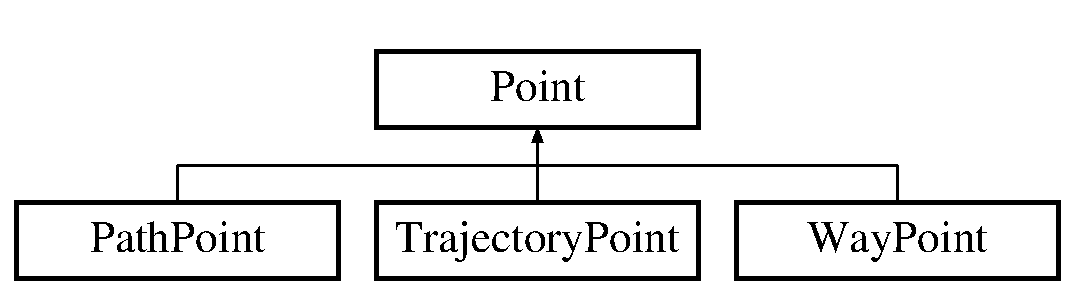
\includegraphics[height=2.000000cm]{classPoint}
\end{center}
\end{figure}
\subsection*{Public Member Functions}
\begin{DoxyCompactItemize}
\item 
\hyperlink{classPoint_ad92f2337b839a94ce97dcdb439b4325a}{Point} ()
\item 
virtual \hyperlink{classPoint_a395fa04b4ec126b66fc053f829a30cc1}{$\sim$\-Point} ()
\item 
void \hyperlink{classPoint_a9c48c0459d14654e7c69e234c82daf2c}{set\-Position} (const \hyperlink{classMotorPosition}{Motor\-Position} \&pos)
\begin{DoxyCompactList}\small\item\em Set the position of a generic \hyperlink{classPoint}{Point} object. \end{DoxyCompactList}\item 
\hyperlink{classMotorPosition}{Motor\-Position} \hyperlink{classPoint_a91c04983e9805cd26751ac03135f9f21}{get\-Position} ()
\begin{DoxyCompactList}\small\item\em Get the previously set position of a generic \hyperlink{classPoint}{Point} object. \end{DoxyCompactList}\item 
void \hyperlink{classPoint_a2cc92f1333e1c9f3cabfb02243d7e65a}{show} ()
\begin{DoxyCompactList}\small\item\em Show the point's position (in motor rotations) \end{DoxyCompactList}\end{DoxyCompactItemize}
\subsection*{Protected Attributes}
\begin{DoxyCompactItemize}
\item 
\hyperlink{classMotorPosition}{Motor\-Position} \hyperlink{classPoint_aedadeabf6bc6500d73d631a355014ff9}{position}
\end{DoxyCompactItemize}


\subsection{Detailed Description}
A point is position reference for a motor. 

\subsection{Constructor \& Destructor Documentation}
\hypertarget{classPoint_ad92f2337b839a94ce97dcdb439b4325a}{\index{Point@{Point}!Point@{Point}}
\index{Point@{Point}!Point@{Point}}
\subsubsection[{Point}]{\setlength{\rightskip}{0pt plus 5cm}Point\-::\-Point (
\begin{DoxyParamCaption}
{}
\end{DoxyParamCaption}
)}}\label{classPoint_ad92f2337b839a94ce97dcdb439b4325a}
\hypertarget{classPoint_a395fa04b4ec126b66fc053f829a30cc1}{\index{Point@{Point}!$\sim$\-Point@{$\sim$\-Point}}
\index{$\sim$\-Point@{$\sim$\-Point}!Point@{Point}}
\subsubsection[{$\sim$\-Point}]{\setlength{\rightskip}{0pt plus 5cm}Point\-::$\sim$\-Point (
\begin{DoxyParamCaption}
{}
\end{DoxyParamCaption}
)\hspace{0.3cm}{\ttfamily [virtual]}}}\label{classPoint_a395fa04b4ec126b66fc053f829a30cc1}


\subsection{Member Function Documentation}
\hypertarget{classPoint_a91c04983e9805cd26751ac03135f9f21}{\index{Point@{Point}!get\-Position@{get\-Position}}
\index{get\-Position@{get\-Position}!Point@{Point}}
\subsubsection[{get\-Position}]{\setlength{\rightskip}{0pt plus 5cm}{\bf Motor\-Position} Point\-::get\-Position (
\begin{DoxyParamCaption}
{}
\end{DoxyParamCaption}
)}}\label{classPoint_a91c04983e9805cd26751ac03135f9f21}


Get the previously set position of a generic \hyperlink{classPoint}{Point} object. 

\begin{DoxyReturn}{Returns}
\hyperlink{classMotorPosition}{Motor\-Position} position of this point 
\end{DoxyReturn}
\hypertarget{classPoint_a9c48c0459d14654e7c69e234c82daf2c}{\index{Point@{Point}!set\-Position@{set\-Position}}
\index{set\-Position@{set\-Position}!Point@{Point}}
\subsubsection[{set\-Position}]{\setlength{\rightskip}{0pt plus 5cm}void Point\-::set\-Position (
\begin{DoxyParamCaption}
\item[{const {\bf Motor\-Position} \&}]{pos}
\end{DoxyParamCaption}
)}}\label{classPoint_a9c48c0459d14654e7c69e234c82daf2c}


Set the position of a generic \hyperlink{classPoint}{Point} object. 


\begin{DoxyParams}[1]{Parameters}
\mbox{\tt in}  & {\em \hyperlink{classMotorPosition}{Motor\-Position}} & pos is a point referenced by a motor position \\
\hline
\end{DoxyParams}
\hypertarget{classPoint_a2cc92f1333e1c9f3cabfb02243d7e65a}{\index{Point@{Point}!show@{show}}
\index{show@{show}!Point@{Point}}
\subsubsection[{show}]{\setlength{\rightskip}{0pt plus 5cm}void Point\-::show (
\begin{DoxyParamCaption}
{}
\end{DoxyParamCaption}
)}}\label{classPoint_a2cc92f1333e1c9f3cabfb02243d7e65a}


Show the point's position (in motor rotations) 



\subsection{Member Data Documentation}
\hypertarget{classPoint_aedadeabf6bc6500d73d631a355014ff9}{\index{Point@{Point}!position@{position}}
\index{position@{position}!Point@{Point}}
\subsubsection[{position}]{\setlength{\rightskip}{0pt plus 5cm}{\bf Motor\-Position} Point\-::position\hspace{0.3cm}{\ttfamily [protected]}}}\label{classPoint_aedadeabf6bc6500d73d631a355014ff9}


The documentation for this class was generated from the following files\-:\begin{DoxyCompactItemize}
\item 
framework/\hyperlink{Point_8hpp}{Point.\-hpp}\item 
framework/\hyperlink{Point_8cpp}{Point.\-cpp}\end{DoxyCompactItemize}

\hypertarget{classRoute}{\section{Route Class Reference}
\label{classRoute}\index{Route@{Route}}
}


A \hyperlink{classRoute}{Route} represents a series of Way Points to be traveled to.  




{\ttfamily \#include $<$Route.\-hpp$>$}

\subsection*{Public Member Functions}
\begin{DoxyCompactItemize}
\item 
\hyperlink{classRoute_a2b1c971aaf032109cee8081c97e9b9e9}{Route} ()
\item 
virtual \hyperlink{classRoute_a41212532f2bce3298d8f9468f82c62ab}{$\sim$\-Route} ()
\item 
void \hyperlink{classRoute_a9411954ba50c930277bbb52ba3f3e7f4}{add\-Way\-Point} (const \hyperlink{classWayPoint}{Way\-Point} \&way\-Point)
\begin{DoxyCompactList}\small\item\em Add a way point to this route. \end{DoxyCompactList}\item 
\hyperlink{classPath}{Path} \hyperlink{classRoute_a05753c003e81efbe2149ad2f1782d70e}{plan\-Path} (const \hyperlink{classMotorVelocity}{Motor\-Velocity} \&max\-Velocity, const \hyperlink{classMotorAcceleration}{Motor\-Acceleration} \&max\-Acceleration)
\begin{DoxyCompactList}\small\item\em Plan a path based on this route's way points. \end{DoxyCompactList}\item 
void \hyperlink{classRoute_a42290dd852c117fe9549bc63c0b4171c}{show} ()
\begin{DoxyCompactList}\small\item\em Show the details of this route on the default output device. \end{DoxyCompactList}\end{DoxyCompactItemize}
\subsection*{Private Attributes}
\begin{DoxyCompactItemize}
\item 
std\-::vector$<$ \hyperlink{classWayPoint}{Way\-Point} $>$ \hyperlink{classRoute_af5aac5eed6cc4fbcd02e2e817d87db45}{route}
\end{DoxyCompactItemize}


\subsection{Detailed Description}
A \hyperlink{classRoute}{Route} represents a series of Way Points to be traveled to. 

\subsection{Constructor \& Destructor Documentation}
\hypertarget{classRoute_a2b1c971aaf032109cee8081c97e9b9e9}{\index{Route@{Route}!Route@{Route}}
\index{Route@{Route}!Route@{Route}}
\subsubsection[{Route}]{\setlength{\rightskip}{0pt plus 5cm}Route\-::\-Route (
\begin{DoxyParamCaption}
{}
\end{DoxyParamCaption}
)}}\label{classRoute_a2b1c971aaf032109cee8081c97e9b9e9}
\hypertarget{classRoute_a41212532f2bce3298d8f9468f82c62ab}{\index{Route@{Route}!$\sim$\-Route@{$\sim$\-Route}}
\index{$\sim$\-Route@{$\sim$\-Route}!Route@{Route}}
\subsubsection[{$\sim$\-Route}]{\setlength{\rightskip}{0pt plus 5cm}Route\-::$\sim$\-Route (
\begin{DoxyParamCaption}
{}
\end{DoxyParamCaption}
)\hspace{0.3cm}{\ttfamily [virtual]}}}\label{classRoute_a41212532f2bce3298d8f9468f82c62ab}


\subsection{Member Function Documentation}
\hypertarget{classRoute_a9411954ba50c930277bbb52ba3f3e7f4}{\index{Route@{Route}!add\-Way\-Point@{add\-Way\-Point}}
\index{add\-Way\-Point@{add\-Way\-Point}!Route@{Route}}
\subsubsection[{add\-Way\-Point}]{\setlength{\rightskip}{0pt plus 5cm}void Route\-::add\-Way\-Point (
\begin{DoxyParamCaption}
\item[{const {\bf Way\-Point} \&}]{way\-Point}
\end{DoxyParamCaption}
)}}\label{classRoute_a9411954ba50c930277bbb52ba3f3e7f4}


Add a way point to this route. 


\begin{DoxyParams}[1]{Parameters}
\mbox{\tt in}  & {\em a} & \hyperlink{classWayPoint}{Way\-Point} to be added to this route \\
\hline
\end{DoxyParams}
\hypertarget{classRoute_a05753c003e81efbe2149ad2f1782d70e}{\index{Route@{Route}!plan\-Path@{plan\-Path}}
\index{plan\-Path@{plan\-Path}!Route@{Route}}
\subsubsection[{plan\-Path}]{\setlength{\rightskip}{0pt plus 5cm}{\bf Path} Route\-::plan\-Path (
\begin{DoxyParamCaption}
\item[{const {\bf Motor\-Velocity} \&}]{max\-Velocity, }
\item[{const {\bf Motor\-Acceleration} \&}]{max\-Acceleration}
\end{DoxyParamCaption}
)}}\label{classRoute_a05753c003e81efbe2149ad2f1782d70e}


Plan a path based on this route's way points. 


\begin{DoxyParams}{Parameters}
{\em max\-Velocity} & \\
\hline
{\em max\-Acceleration} & \\
\hline
\end{DoxyParams}
\begin{DoxyReturn}{Returns}
a \hyperlink{classPath}{Path} object specifying the path points to traverse 
\end{DoxyReturn}
\hypertarget{classRoute_a42290dd852c117fe9549bc63c0b4171c}{\index{Route@{Route}!show@{show}}
\index{show@{show}!Route@{Route}}
\subsubsection[{show}]{\setlength{\rightskip}{0pt plus 5cm}void Route\-::show (
\begin{DoxyParamCaption}
{}
\end{DoxyParamCaption}
)}}\label{classRoute_a42290dd852c117fe9549bc63c0b4171c}


Show the details of this route on the default output device. 



\subsection{Member Data Documentation}
\hypertarget{classRoute_af5aac5eed6cc4fbcd02e2e817d87db45}{\index{Route@{Route}!route@{route}}
\index{route@{route}!Route@{Route}}
\subsubsection[{route}]{\setlength{\rightskip}{0pt plus 5cm}std\-::vector$<${\bf Way\-Point}$>$ Route\-::route\hspace{0.3cm}{\ttfamily [private]}}}\label{classRoute_af5aac5eed6cc4fbcd02e2e817d87db45}


The documentation for this class was generated from the following files\-:\begin{DoxyCompactItemize}
\item 
framework/\hyperlink{Route_8hpp}{Route.\-hpp}\item 
framework/\hyperlink{Route_8cpp}{Route.\-cpp}\end{DoxyCompactItemize}

\hypertarget{classTankDrive}{\section{Tank\-Drive Class Reference}
\label{classTankDrive}\index{Tank\-Drive@{Tank\-Drive}}
}


\hyperlink{classTankDrive}{Tank\-Drive} is derived from the base class \hyperlink{classDriveSystem}{Drive\-System}.  




{\ttfamily \#include $<$Tank\-Drive.\-hpp$>$}

Inheritance diagram for Tank\-Drive\-:\begin{figure}[H]
\begin{center}
\leavevmode
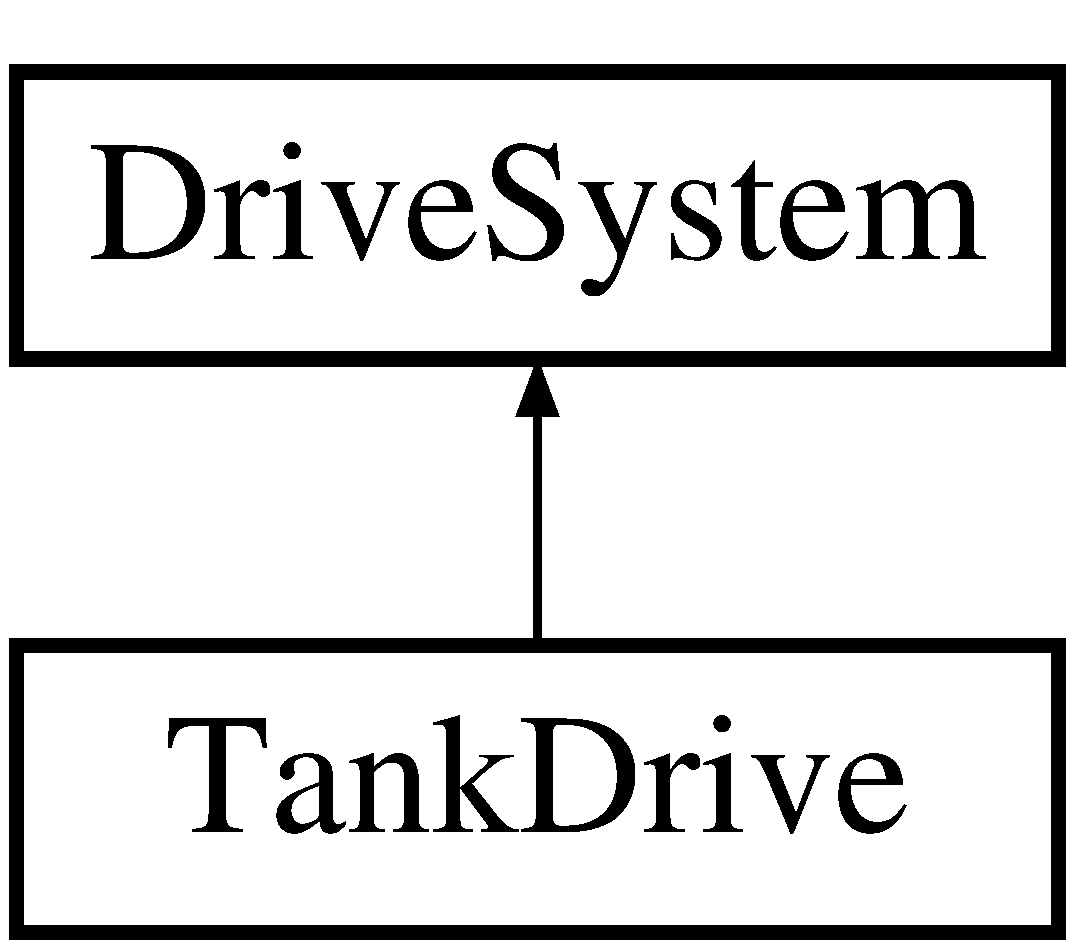
\includegraphics[height=2.000000cm]{classTankDrive}
\end{center}
\end{figure}
\subsection*{Public Member Functions}
\begin{DoxyCompactItemize}
\item 
\hyperlink{classTankDrive_aa60aae817ddee667161e9fa4e65b164c}{Tank\-Drive} ()
\item 
virtual \hyperlink{classTankDrive_a56b6753b731ed996eee30da3e0d44055}{$\sim$\-Tank\-Drive} ()
\item 
void \hyperlink{classTankDrive_ab425ff9f2e12317fb45253da80886915}{set\-Width\-In\-Feet} (double width)
\begin{DoxyCompactList}\small\item\em Set the distance between the two \hyperlink{classTankDrive}{Tank\-Drive} motivators (left and right sides) \end{DoxyCompactList}\item 
double \hyperlink{classTankDrive_a1d755a00437ccfa2e5e12634f473ac30}{get\-Width\-In\-Feet} ()
\begin{DoxyCompactList}\small\item\em Get the distance between the two \hyperlink{classTankDrive}{Tank\-Drive} motivators (left and right sides) \end{DoxyCompactList}\item 
void \hyperlink{classTankDrive_ab4f103bfd11ab28c18ef292a505c454e}{move} (double distance\-Feet, \hyperlink{classChassisTurnRate}{Chassis\-Turn\-Rate} chassis\-Turn\-Rate, \hyperlink{classChassisVelocity}{Chassis\-Velocity} chassis\-Velocity\-Requested, \hyperlink{classChassisAcceleration}{Chassis\-Acceleration} chassis\-Acceleleration\-Requested)
\begin{DoxyCompactList}\small\item\em Move the \hyperlink{classTankDrive}{Tank\-Drive} according to the movement parameters. \end{DoxyCompactList}\end{DoxyCompactItemize}
\subsection*{Private Attributes}
\begin{DoxyCompactItemize}
\item 
double \hyperlink{classTankDrive_a4c4b4e59f8fbfa31115aa3aa03c04d31}{width\-In\-Feet}
\end{DoxyCompactItemize}
\subsection*{Additional Inherited Members}


\subsection{Detailed Description}
\hyperlink{classTankDrive}{Tank\-Drive} is derived from the base class \hyperlink{classDriveSystem}{Drive\-System}. 

\subsection{Constructor \& Destructor Documentation}
\hypertarget{classTankDrive_aa60aae817ddee667161e9fa4e65b164c}{\index{Tank\-Drive@{Tank\-Drive}!Tank\-Drive@{Tank\-Drive}}
\index{Tank\-Drive@{Tank\-Drive}!TankDrive@{Tank\-Drive}}
\subsubsection[{Tank\-Drive}]{\setlength{\rightskip}{0pt plus 5cm}Tank\-Drive\-::\-Tank\-Drive (
\begin{DoxyParamCaption}
{}
\end{DoxyParamCaption}
)}}\label{classTankDrive_aa60aae817ddee667161e9fa4e65b164c}
\hypertarget{classTankDrive_a56b6753b731ed996eee30da3e0d44055}{\index{Tank\-Drive@{Tank\-Drive}!$\sim$\-Tank\-Drive@{$\sim$\-Tank\-Drive}}
\index{$\sim$\-Tank\-Drive@{$\sim$\-Tank\-Drive}!TankDrive@{Tank\-Drive}}
\subsubsection[{$\sim$\-Tank\-Drive}]{\setlength{\rightskip}{0pt plus 5cm}Tank\-Drive\-::$\sim$\-Tank\-Drive (
\begin{DoxyParamCaption}
{}
\end{DoxyParamCaption}
)\hspace{0.3cm}{\ttfamily [virtual]}}}\label{classTankDrive_a56b6753b731ed996eee30da3e0d44055}


\subsection{Member Function Documentation}
\hypertarget{classTankDrive_a1d755a00437ccfa2e5e12634f473ac30}{\index{Tank\-Drive@{Tank\-Drive}!get\-Width\-In\-Feet@{get\-Width\-In\-Feet}}
\index{get\-Width\-In\-Feet@{get\-Width\-In\-Feet}!TankDrive@{Tank\-Drive}}
\subsubsection[{get\-Width\-In\-Feet}]{\setlength{\rightskip}{0pt plus 5cm}double Tank\-Drive\-::get\-Width\-In\-Feet (
\begin{DoxyParamCaption}
{}
\end{DoxyParamCaption}
)}}\label{classTankDrive_a1d755a00437ccfa2e5e12634f473ac30}


Get the distance between the two \hyperlink{classTankDrive}{Tank\-Drive} motivators (left and right sides) 

\begin{DoxyReturn}{Returns}
double width as the distance between the two \hyperlink{classTankDrive}{Tank\-Drive} motivators (left and right sides) 
\end{DoxyReturn}
\hypertarget{classTankDrive_ab4f103bfd11ab28c18ef292a505c454e}{\index{Tank\-Drive@{Tank\-Drive}!move@{move}}
\index{move@{move}!TankDrive@{Tank\-Drive}}
\subsubsection[{move}]{\setlength{\rightskip}{0pt plus 5cm}void Tank\-Drive\-::move (
\begin{DoxyParamCaption}
\item[{double}]{distance\-Feet, }
\item[{{\bf Chassis\-Turn\-Rate}}]{chassis\-Turn\-Rate, }
\item[{{\bf Chassis\-Velocity}}]{chassis\-Velocity\-Requested, }
\item[{{\bf Chassis\-Acceleration}}]{chassis\-Acceleration\-Requested}
\end{DoxyParamCaption}
)\hspace{0.3cm}{\ttfamily [virtual]}}}\label{classTankDrive_ab4f103bfd11ab28c18ef292a505c454e}


Move the \hyperlink{classTankDrive}{Tank\-Drive} according to the movement parameters. 


\begin{DoxyParams}[1]{Parameters}
\mbox{\tt in}  & {\em double} & distance\-Feet -\/ distance to move in feet \\
\hline
 & {\em \hyperlink{classChassisTurnRate}{Chassis\-Turn\-Rate}} & chassis\-Turn\-Rate -\/ go straight or change heading as moving \\
\hline
 & {\em \hyperlink{classChassisVelocity}{Chassis\-Velocity}} & chassis\-Velocity\-Requested -\/ move at this rate \\
\hline
 & {\em \hyperlink{classChassisAcceleration}{Chassis\-Acceleration}} & chassis\-Acceleration\-Requested -\/ accelerate at this rate \\
\hline
\end{DoxyParams}


Reimplemented from \hyperlink{classDriveSystem_af0f174a092b6b4a13ae589a1d72ff0c8}{Drive\-System}.

\hypertarget{classTankDrive_ab425ff9f2e12317fb45253da80886915}{\index{Tank\-Drive@{Tank\-Drive}!set\-Width\-In\-Feet@{set\-Width\-In\-Feet}}
\index{set\-Width\-In\-Feet@{set\-Width\-In\-Feet}!TankDrive@{Tank\-Drive}}
\subsubsection[{set\-Width\-In\-Feet}]{\setlength{\rightskip}{0pt plus 5cm}void Tank\-Drive\-::set\-Width\-In\-Feet (
\begin{DoxyParamCaption}
\item[{double}]{width}
\end{DoxyParamCaption}
)}}\label{classTankDrive_ab425ff9f2e12317fb45253da80886915}


Set the distance between the two \hyperlink{classTankDrive}{Tank\-Drive} motivators (left and right sides) 


\begin{DoxyParams}[1]{Parameters}
\mbox{\tt in}  & {\em double} & width as the distance between the two \hyperlink{classTankDrive}{Tank\-Drive} motivators (left and right sides) \\
\hline
\end{DoxyParams}


\subsection{Member Data Documentation}
\hypertarget{classTankDrive_a4c4b4e59f8fbfa31115aa3aa03c04d31}{\index{Tank\-Drive@{Tank\-Drive}!width\-In\-Feet@{width\-In\-Feet}}
\index{width\-In\-Feet@{width\-In\-Feet}!TankDrive@{Tank\-Drive}}
\subsubsection[{width\-In\-Feet}]{\setlength{\rightskip}{0pt plus 5cm}double Tank\-Drive\-::width\-In\-Feet\hspace{0.3cm}{\ttfamily [private]}}}\label{classTankDrive_a4c4b4e59f8fbfa31115aa3aa03c04d31}


The documentation for this class was generated from the following files\-:\begin{DoxyCompactItemize}
\item 
framework/\hyperlink{TankDrive_8hpp}{Tank\-Drive.\-hpp}\item 
framework/\hyperlink{TankDrive_8cpp}{Tank\-Drive.\-cpp}\end{DoxyCompactItemize}

\hypertarget{classTrajectory}{\section{Trajectory Class Reference}
\label{classTrajectory}\index{Trajectory@{Trajectory}}
}


A trajectory is a vector of motion profile trajectory points.  




{\ttfamily \#include $<$Trajectory.\-hpp$>$}

\subsection*{Public Member Functions}
\begin{DoxyCompactItemize}
\item 
\hyperlink{classTrajectory_aa340ba80f1f4d1aa39f19f069d5d8089}{Trajectory} ()
\item 
virtual \hyperlink{classTrajectory_ac673c37025ca5353ad99ab41c936e75d}{$\sim$\-Trajectory} ()
\item 
\hyperlink{classMotorVelocity}{Motor\-Velocity} \hyperlink{classTrajectory_a6b978d0ab6ef13bbf3034b1f6d37180b}{get\-Max\-Velocity} ()
\begin{DoxyCompactList}\small\item\em Get the maximum velocity for this trajectory. \end{DoxyCompactList}\item 
\hyperlink{classMotorAcceleration}{Motor\-Acceleration} \hyperlink{classTrajectory_ad05719b4fb4d03288ea1adb8c110059c}{get\-Max\-Acceleration} ()
\begin{DoxyCompactList}\small\item\em Get the maximum acceleration for this trajectory. \end{DoxyCompactList}\item 
\hyperlink{classMotorPosition}{Motor\-Position} \hyperlink{classTrajectory_a03e1d57ceece06e7af1250bcc72ae265}{get\-Distance} ()
\begin{DoxyCompactList}\small\item\em Get the distance covered by this trajectory (in \hyperlink{classMotorPosition}{Motor\-Position} units) \end{DoxyCompactList}\item 
unsigned int \hyperlink{classTrajectory_a6b8d62dd1ce207ce77eb1fe5e7937f2c}{get\-Algo\-It\-P\-M\-S} ()
\begin{DoxyCompactList}\small\item\em Get the iteration period for this trajectory in milliseconds. \end{DoxyCompactList}\item 
unsigned int \hyperlink{classTrajectory_a8aebfcf3c5519b0350e82df8d8a24c5c}{get\-Algo\-T1\-M\-S} ()
\begin{DoxyCompactList}\small\item\em Get the algorithmic variable T1 for this trajectory in milliseconds. \end{DoxyCompactList}\item 
unsigned int \hyperlink{classTrajectory_a21342821f9027d423baa6b9a07828421}{get\-Algo\-T2\-M\-S} ()
\begin{DoxyCompactList}\small\item\em Get the algorithmic variable T2 for this trajectory in milliseconds. \end{DoxyCompactList}\item 
unsigned int \hyperlink{classTrajectory_a61122874889996b7c31cd268b8f45a9a}{get\-Algo\-T4\-M\-S} ()
\begin{DoxyCompactList}\small\item\em Get the algorithmic variable T4 for this trajectory in milliseconds. \end{DoxyCompactList}\item 
unsigned int \hyperlink{classTrajectory_a7db227eff10e1b65c706f9059380af96}{get\-Algo\-F\-L1count} ()
\begin{DoxyCompactList}\small\item\em Get the algorithmic variable F\-L1 for this trajectory as a count. \end{DoxyCompactList}\item 
unsigned int \hyperlink{classTrajectory_ab2406c8e1fbde1523d8ff47bafcfea2b}{get\-Algo\-F\-L2count} ()
\begin{DoxyCompactList}\small\item\em Get the algorithmic variable F\-L2 for this trajectory as a count. \end{DoxyCompactList}\item 
unsigned int \hyperlink{classTrajectory_a818f34c118496aecc5637a672b482d64}{get\-Algo\-Ncount} ()
\begin{DoxyCompactList}\small\item\em Get the algorithmic variable N for this trajectory as a count. \end{DoxyCompactList}\item 
void \hyperlink{classTrajectory_af536bb24d9009ebaa58ec3eb4e415a96}{generate} (\hyperlink{classPath}{Path} \&path, const unsigned int iteration\-Period\-M\-S)
\begin{DoxyCompactList}\small\item\em Generate a trajectory based on a provided 2-\/point path. \end{DoxyCompactList}\item 
void \hyperlink{classTrajectory_a54a11d19ae655d4db78ecd59d0d5a131}{execute} ()
\begin{DoxyCompactList}\small\item\em Stub Execution of this trajectory's motion profile trajectory points. \end{DoxyCompactList}\item 
unsigned int \hyperlink{classTrajectory_a93083e57d71d95670b957aa31aacab25}{size} ()
\begin{DoxyCompactList}\small\item\em Returns the number of points in the motion profile trajectory. \end{DoxyCompactList}\item 
void \hyperlink{classTrajectory_aaedb75c528c178cee1023a74f2caa077}{show} ()
\begin{DoxyCompactList}\small\item\em Show this motion profile trajectory as individual points. \end{DoxyCompactList}\item 
void \hyperlink{classTrajectory_a78f10564618041f74666a5dbb735e4cb}{output\-C\-S\-V} (const std\-::string \&trajectory\-File\-Name)
\begin{DoxyCompactList}\small\item\em Output this motion profile trajectory as data to a C\-S\-V file. \end{DoxyCompactList}\end{DoxyCompactItemize}
\subsection*{Private Member Functions}
\begin{DoxyCompactItemize}
\item 
void \hyperlink{classTrajectory_a76e24db532647bd0d5e3ba1e004d85ee}{add\-To\-History} (std\-::vector$<$ double $>$ \&history, const unsigned int max, const double value)
\begin{DoxyCompactList}\small\item\em Private function to maintain a limited history of double values. \end{DoxyCompactList}\end{DoxyCompactItemize}
\subsection*{Private Attributes}
\begin{DoxyCompactItemize}
\item 
\hyperlink{classMotorVelocity}{Motor\-Velocity} \hyperlink{classTrajectory_a7101fccd21bccbf6ff66ae855fc6fb04}{max\-Velocity}
\item 
\hyperlink{classMotorAcceleration}{Motor\-Acceleration} \hyperlink{classTrajectory_aff0221bf2932e63c3b1211cacb273dc6}{max\-Acceleration}
\item 
\hyperlink{classMotorPosition}{Motor\-Position} \hyperlink{classTrajectory_adca462e882c89640c83cb546294ec6c8}{distance}
\item 
unsigned int \hyperlink{classTrajectory_a6fcb37a2f4d0ba6c79bacbe74c8c8291}{algo\-It\-P\-M\-S}
\item 
unsigned int \hyperlink{classTrajectory_a47305aeb6de4a4102406db6111e155d6}{algo\-T1\-M\-S}
\item 
unsigned int \hyperlink{classTrajectory_ada35c0fd4e7de5e9eec428e800d045e6}{algo\-T2\-M\-S}
\item 
unsigned int \hyperlink{classTrajectory_a7e8f6a0075794037354ad92416131be3}{algo\-T4\-M\-S}
\item 
unsigned int \hyperlink{classTrajectory_a6821dd2945918f2307a4004319050369}{algo\-F\-L1count}
\item 
unsigned int \hyperlink{classTrajectory_a56c679a5deca7efadc9c957f3e418e7b}{algo\-F\-L2count}
\item 
unsigned int \hyperlink{classTrajectory_a130dbb1855dd1ac27f89c6f9c30fe019}{algo\-Ncount}
\item 
std\-::vector$<$ \hyperlink{classTrajectoryPoint}{Trajectory\-Point} $>$ \hyperlink{classTrajectory_a159e6800353ba91aa66f304de8fa177c}{trajectory}
\end{DoxyCompactItemize}


\subsection{Detailed Description}
A trajectory is a vector of motion profile trajectory points. 

\subsection{Constructor \& Destructor Documentation}
\hypertarget{classTrajectory_aa340ba80f1f4d1aa39f19f069d5d8089}{\index{Trajectory@{Trajectory}!Trajectory@{Trajectory}}
\index{Trajectory@{Trajectory}!Trajectory@{Trajectory}}
\subsubsection[{Trajectory}]{\setlength{\rightskip}{0pt plus 5cm}Trajectory\-::\-Trajectory (
\begin{DoxyParamCaption}
{}
\end{DoxyParamCaption}
)}}\label{classTrajectory_aa340ba80f1f4d1aa39f19f069d5d8089}
\hypertarget{classTrajectory_ac673c37025ca5353ad99ab41c936e75d}{\index{Trajectory@{Trajectory}!$\sim$\-Trajectory@{$\sim$\-Trajectory}}
\index{$\sim$\-Trajectory@{$\sim$\-Trajectory}!Trajectory@{Trajectory}}
\subsubsection[{$\sim$\-Trajectory}]{\setlength{\rightskip}{0pt plus 5cm}Trajectory\-::$\sim$\-Trajectory (
\begin{DoxyParamCaption}
{}
\end{DoxyParamCaption}
)\hspace{0.3cm}{\ttfamily [virtual]}}}\label{classTrajectory_ac673c37025ca5353ad99ab41c936e75d}


\subsection{Member Function Documentation}
\hypertarget{classTrajectory_a76e24db532647bd0d5e3ba1e004d85ee}{\index{Trajectory@{Trajectory}!add\-To\-History@{add\-To\-History}}
\index{add\-To\-History@{add\-To\-History}!Trajectory@{Trajectory}}
\subsubsection[{add\-To\-History}]{\setlength{\rightskip}{0pt plus 5cm}void Trajectory\-::add\-To\-History (
\begin{DoxyParamCaption}
\item[{std\-::vector$<$ double $>$ \&}]{history, }
\item[{const unsigned int}]{max, }
\item[{const double}]{value}
\end{DoxyParamCaption}
)\hspace{0.3cm}{\ttfamily [private]}}}\label{classTrajectory_a76e24db532647bd0d5e3ba1e004d85ee}


Private function to maintain a limited history of double values. 


\begin{DoxyParams}[1]{Parameters}
 & {\em \mbox{[}in/out\mbox{]}} & vector$<$double$>$ history of values \\
\hline
\mbox{\tt in}  & {\em unsigned} & int maximum number of values to keep in the history list \\
\hline
\mbox{\tt in}  & {\em double} & value to add to the list \\
\hline
\end{DoxyParams}
\hypertarget{classTrajectory_a54a11d19ae655d4db78ecd59d0d5a131}{\index{Trajectory@{Trajectory}!execute@{execute}}
\index{execute@{execute}!Trajectory@{Trajectory}}
\subsubsection[{execute}]{\setlength{\rightskip}{0pt plus 5cm}void Trajectory\-::execute (
\begin{DoxyParamCaption}
{}
\end{DoxyParamCaption}
)}}\label{classTrajectory_a54a11d19ae655d4db78ecd59d0d5a131}


Stub Execution of this trajectory's motion profile trajectory points. 

\hypertarget{classTrajectory_af536bb24d9009ebaa58ec3eb4e415a96}{\index{Trajectory@{Trajectory}!generate@{generate}}
\index{generate@{generate}!Trajectory@{Trajectory}}
\subsubsection[{generate}]{\setlength{\rightskip}{0pt plus 5cm}void Trajectory\-::generate (
\begin{DoxyParamCaption}
\item[{{\bf Path} \&}]{path, }
\item[{const unsigned int}]{iteration\-Period\-M\-S}
\end{DoxyParamCaption}
)}}\label{classTrajectory_af536bb24d9009ebaa58ec3eb4e415a96}


Generate a trajectory based on a provided 2-\/point path. 


\begin{DoxyParams}[1]{Parameters}
\mbox{\tt in}  & {\em path} & A motion path consisting of a series of path points \\
\hline
\mbox{\tt in}  & {\em unsigned} & int iteration period in milliseconds (time slice for execution of each trajectory point) \\
\hline
\end{DoxyParams}
\hypertarget{classTrajectory_a7db227eff10e1b65c706f9059380af96}{\index{Trajectory@{Trajectory}!get\-Algo\-F\-L1count@{get\-Algo\-F\-L1count}}
\index{get\-Algo\-F\-L1count@{get\-Algo\-F\-L1count}!Trajectory@{Trajectory}}
\subsubsection[{get\-Algo\-F\-L1count}]{\setlength{\rightskip}{0pt plus 5cm}unsigned int Trajectory\-::get\-Algo\-F\-L1count (
\begin{DoxyParamCaption}
{}
\end{DoxyParamCaption}
)}}\label{classTrajectory_a7db227eff10e1b65c706f9059380af96}


Get the algorithmic variable F\-L1 for this trajectory as a count. 

\begin{DoxyReturn}{Returns}
int algorithmic variable F\-L1 for this trajectory as a count 
\end{DoxyReturn}
\hypertarget{classTrajectory_ab2406c8e1fbde1523d8ff47bafcfea2b}{\index{Trajectory@{Trajectory}!get\-Algo\-F\-L2count@{get\-Algo\-F\-L2count}}
\index{get\-Algo\-F\-L2count@{get\-Algo\-F\-L2count}!Trajectory@{Trajectory}}
\subsubsection[{get\-Algo\-F\-L2count}]{\setlength{\rightskip}{0pt plus 5cm}unsigned int Trajectory\-::get\-Algo\-F\-L2count (
\begin{DoxyParamCaption}
{}
\end{DoxyParamCaption}
)}}\label{classTrajectory_ab2406c8e1fbde1523d8ff47bafcfea2b}


Get the algorithmic variable F\-L2 for this trajectory as a count. 

\begin{DoxyReturn}{Returns}
int algorithmic variable F\-L2 for this trajectory as a count 
\end{DoxyReturn}
\hypertarget{classTrajectory_a6b8d62dd1ce207ce77eb1fe5e7937f2c}{\index{Trajectory@{Trajectory}!get\-Algo\-It\-P\-M\-S@{get\-Algo\-It\-P\-M\-S}}
\index{get\-Algo\-It\-P\-M\-S@{get\-Algo\-It\-P\-M\-S}!Trajectory@{Trajectory}}
\subsubsection[{get\-Algo\-It\-P\-M\-S}]{\setlength{\rightskip}{0pt plus 5cm}unsigned int Trajectory\-::get\-Algo\-It\-P\-M\-S (
\begin{DoxyParamCaption}
{}
\end{DoxyParamCaption}
)}}\label{classTrajectory_a6b8d62dd1ce207ce77eb1fe5e7937f2c}


Get the iteration period for this trajectory in milliseconds. 

\begin{DoxyReturn}{Returns}
int iteration period in milliseconds 
\end{DoxyReturn}
\hypertarget{classTrajectory_a818f34c118496aecc5637a672b482d64}{\index{Trajectory@{Trajectory}!get\-Algo\-Ncount@{get\-Algo\-Ncount}}
\index{get\-Algo\-Ncount@{get\-Algo\-Ncount}!Trajectory@{Trajectory}}
\subsubsection[{get\-Algo\-Ncount}]{\setlength{\rightskip}{0pt plus 5cm}unsigned int Trajectory\-::get\-Algo\-Ncount (
\begin{DoxyParamCaption}
{}
\end{DoxyParamCaption}
)}}\label{classTrajectory_a818f34c118496aecc5637a672b482d64}


Get the algorithmic variable N for this trajectory as a count. 

\begin{DoxyReturn}{Returns}
int algorithmic variable N for this trajectory as a count 
\end{DoxyReturn}
\hypertarget{classTrajectory_a8aebfcf3c5519b0350e82df8d8a24c5c}{\index{Trajectory@{Trajectory}!get\-Algo\-T1\-M\-S@{get\-Algo\-T1\-M\-S}}
\index{get\-Algo\-T1\-M\-S@{get\-Algo\-T1\-M\-S}!Trajectory@{Trajectory}}
\subsubsection[{get\-Algo\-T1\-M\-S}]{\setlength{\rightskip}{0pt plus 5cm}unsigned int Trajectory\-::get\-Algo\-T1\-M\-S (
\begin{DoxyParamCaption}
{}
\end{DoxyParamCaption}
)}}\label{classTrajectory_a8aebfcf3c5519b0350e82df8d8a24c5c}


Get the algorithmic variable T1 for this trajectory in milliseconds. 

\begin{DoxyReturn}{Returns}
int algorithmic variable T1 for this trajectory in milliseconds 
\end{DoxyReturn}
\hypertarget{classTrajectory_a21342821f9027d423baa6b9a07828421}{\index{Trajectory@{Trajectory}!get\-Algo\-T2\-M\-S@{get\-Algo\-T2\-M\-S}}
\index{get\-Algo\-T2\-M\-S@{get\-Algo\-T2\-M\-S}!Trajectory@{Trajectory}}
\subsubsection[{get\-Algo\-T2\-M\-S}]{\setlength{\rightskip}{0pt plus 5cm}unsigned int Trajectory\-::get\-Algo\-T2\-M\-S (
\begin{DoxyParamCaption}
{}
\end{DoxyParamCaption}
)}}\label{classTrajectory_a21342821f9027d423baa6b9a07828421}


Get the algorithmic variable T2 for this trajectory in milliseconds. 

\begin{DoxyReturn}{Returns}
int algorithmic variable T2 for this trajectory in milliseconds 
\end{DoxyReturn}
\hypertarget{classTrajectory_a61122874889996b7c31cd268b8f45a9a}{\index{Trajectory@{Trajectory}!get\-Algo\-T4\-M\-S@{get\-Algo\-T4\-M\-S}}
\index{get\-Algo\-T4\-M\-S@{get\-Algo\-T4\-M\-S}!Trajectory@{Trajectory}}
\subsubsection[{get\-Algo\-T4\-M\-S}]{\setlength{\rightskip}{0pt plus 5cm}unsigned int Trajectory\-::get\-Algo\-T4\-M\-S (
\begin{DoxyParamCaption}
{}
\end{DoxyParamCaption}
)}}\label{classTrajectory_a61122874889996b7c31cd268b8f45a9a}


Get the algorithmic variable T4 for this trajectory in milliseconds. 

\begin{DoxyReturn}{Returns}
int algorithmic variable T4 for this trajectory in milliseconds 
\end{DoxyReturn}
\hypertarget{classTrajectory_a03e1d57ceece06e7af1250bcc72ae265}{\index{Trajectory@{Trajectory}!get\-Distance@{get\-Distance}}
\index{get\-Distance@{get\-Distance}!Trajectory@{Trajectory}}
\subsubsection[{get\-Distance}]{\setlength{\rightskip}{0pt plus 5cm}{\bf Motor\-Position} Trajectory\-::get\-Distance (
\begin{DoxyParamCaption}
{}
\end{DoxyParamCaption}
)}}\label{classTrajectory_a03e1d57ceece06e7af1250bcc72ae265}


Get the distance covered by this trajectory (in \hyperlink{classMotorPosition}{Motor\-Position} units) 

\begin{DoxyReturn}{Returns}
a \hyperlink{classMotorPosition}{Motor\-Position} representing this trajectory's distance covered 
\end{DoxyReturn}
\hypertarget{classTrajectory_ad05719b4fb4d03288ea1adb8c110059c}{\index{Trajectory@{Trajectory}!get\-Max\-Acceleration@{get\-Max\-Acceleration}}
\index{get\-Max\-Acceleration@{get\-Max\-Acceleration}!Trajectory@{Trajectory}}
\subsubsection[{get\-Max\-Acceleration}]{\setlength{\rightskip}{0pt plus 5cm}{\bf Motor\-Acceleration} Trajectory\-::get\-Max\-Acceleration (
\begin{DoxyParamCaption}
{}
\end{DoxyParamCaption}
)}}\label{classTrajectory_ad05719b4fb4d03288ea1adb8c110059c}


Get the maximum acceleration for this trajectory. 

\begin{DoxyReturn}{Returns}
a \hyperlink{classMotorAcceleration}{Motor\-Acceleration} representing this trajectory's maximum acceleration 
\end{DoxyReturn}
\hypertarget{classTrajectory_a6b978d0ab6ef13bbf3034b1f6d37180b}{\index{Trajectory@{Trajectory}!get\-Max\-Velocity@{get\-Max\-Velocity}}
\index{get\-Max\-Velocity@{get\-Max\-Velocity}!Trajectory@{Trajectory}}
\subsubsection[{get\-Max\-Velocity}]{\setlength{\rightskip}{0pt plus 5cm}{\bf Motor\-Velocity} Trajectory\-::get\-Max\-Velocity (
\begin{DoxyParamCaption}
{}
\end{DoxyParamCaption}
)}}\label{classTrajectory_a6b978d0ab6ef13bbf3034b1f6d37180b}


Get the maximum velocity for this trajectory. 

\begin{DoxyReturn}{Returns}
a \hyperlink{classMotorVelocity}{Motor\-Velocity} representing this trajectory's maximum velocity 
\end{DoxyReturn}
\hypertarget{classTrajectory_a78f10564618041f74666a5dbb735e4cb}{\index{Trajectory@{Trajectory}!output\-C\-S\-V@{output\-C\-S\-V}}
\index{output\-C\-S\-V@{output\-C\-S\-V}!Trajectory@{Trajectory}}
\subsubsection[{output\-C\-S\-V}]{\setlength{\rightskip}{0pt plus 5cm}void Trajectory\-::output\-C\-S\-V (
\begin{DoxyParamCaption}
\item[{const std\-::string \&}]{trajectory\-File\-Name}
\end{DoxyParamCaption}
)}}\label{classTrajectory_a78f10564618041f74666a5dbb735e4cb}


Output this motion profile trajectory as data to a C\-S\-V file. 

\hypertarget{classTrajectory_aaedb75c528c178cee1023a74f2caa077}{\index{Trajectory@{Trajectory}!show@{show}}
\index{show@{show}!Trajectory@{Trajectory}}
\subsubsection[{show}]{\setlength{\rightskip}{0pt plus 5cm}void Trajectory\-::show (
\begin{DoxyParamCaption}
{}
\end{DoxyParamCaption}
)}}\label{classTrajectory_aaedb75c528c178cee1023a74f2caa077}


Show this motion profile trajectory as individual points. 

\hypertarget{classTrajectory_a93083e57d71d95670b957aa31aacab25}{\index{Trajectory@{Trajectory}!size@{size}}
\index{size@{size}!Trajectory@{Trajectory}}
\subsubsection[{size}]{\setlength{\rightskip}{0pt plus 5cm}unsigned int Trajectory\-::size (
\begin{DoxyParamCaption}
{}
\end{DoxyParamCaption}
)}}\label{classTrajectory_a93083e57d71d95670b957aa31aacab25}


Returns the number of points in the motion profile trajectory. 

\begin{DoxyReturn}{Returns}
int motion profile trajectory size 
\end{DoxyReturn}


\subsection{Member Data Documentation}
\hypertarget{classTrajectory_a6821dd2945918f2307a4004319050369}{\index{Trajectory@{Trajectory}!algo\-F\-L1count@{algo\-F\-L1count}}
\index{algo\-F\-L1count@{algo\-F\-L1count}!Trajectory@{Trajectory}}
\subsubsection[{algo\-F\-L1count}]{\setlength{\rightskip}{0pt plus 5cm}unsigned int Trajectory\-::algo\-F\-L1count\hspace{0.3cm}{\ttfamily [private]}}}\label{classTrajectory_a6821dd2945918f2307a4004319050369}
\hypertarget{classTrajectory_a56c679a5deca7efadc9c957f3e418e7b}{\index{Trajectory@{Trajectory}!algo\-F\-L2count@{algo\-F\-L2count}}
\index{algo\-F\-L2count@{algo\-F\-L2count}!Trajectory@{Trajectory}}
\subsubsection[{algo\-F\-L2count}]{\setlength{\rightskip}{0pt plus 5cm}unsigned int Trajectory\-::algo\-F\-L2count\hspace{0.3cm}{\ttfamily [private]}}}\label{classTrajectory_a56c679a5deca7efadc9c957f3e418e7b}
\hypertarget{classTrajectory_a6fcb37a2f4d0ba6c79bacbe74c8c8291}{\index{Trajectory@{Trajectory}!algo\-It\-P\-M\-S@{algo\-It\-P\-M\-S}}
\index{algo\-It\-P\-M\-S@{algo\-It\-P\-M\-S}!Trajectory@{Trajectory}}
\subsubsection[{algo\-It\-P\-M\-S}]{\setlength{\rightskip}{0pt plus 5cm}unsigned int Trajectory\-::algo\-It\-P\-M\-S\hspace{0.3cm}{\ttfamily [private]}}}\label{classTrajectory_a6fcb37a2f4d0ba6c79bacbe74c8c8291}
\hypertarget{classTrajectory_a130dbb1855dd1ac27f89c6f9c30fe019}{\index{Trajectory@{Trajectory}!algo\-Ncount@{algo\-Ncount}}
\index{algo\-Ncount@{algo\-Ncount}!Trajectory@{Trajectory}}
\subsubsection[{algo\-Ncount}]{\setlength{\rightskip}{0pt plus 5cm}unsigned int Trajectory\-::algo\-Ncount\hspace{0.3cm}{\ttfamily [private]}}}\label{classTrajectory_a130dbb1855dd1ac27f89c6f9c30fe019}
\hypertarget{classTrajectory_a47305aeb6de4a4102406db6111e155d6}{\index{Trajectory@{Trajectory}!algo\-T1\-M\-S@{algo\-T1\-M\-S}}
\index{algo\-T1\-M\-S@{algo\-T1\-M\-S}!Trajectory@{Trajectory}}
\subsubsection[{algo\-T1\-M\-S}]{\setlength{\rightskip}{0pt plus 5cm}unsigned int Trajectory\-::algo\-T1\-M\-S\hspace{0.3cm}{\ttfamily [private]}}}\label{classTrajectory_a47305aeb6de4a4102406db6111e155d6}
\hypertarget{classTrajectory_ada35c0fd4e7de5e9eec428e800d045e6}{\index{Trajectory@{Trajectory}!algo\-T2\-M\-S@{algo\-T2\-M\-S}}
\index{algo\-T2\-M\-S@{algo\-T2\-M\-S}!Trajectory@{Trajectory}}
\subsubsection[{algo\-T2\-M\-S}]{\setlength{\rightskip}{0pt plus 5cm}unsigned int Trajectory\-::algo\-T2\-M\-S\hspace{0.3cm}{\ttfamily [private]}}}\label{classTrajectory_ada35c0fd4e7de5e9eec428e800d045e6}
\hypertarget{classTrajectory_a7e8f6a0075794037354ad92416131be3}{\index{Trajectory@{Trajectory}!algo\-T4\-M\-S@{algo\-T4\-M\-S}}
\index{algo\-T4\-M\-S@{algo\-T4\-M\-S}!Trajectory@{Trajectory}}
\subsubsection[{algo\-T4\-M\-S}]{\setlength{\rightskip}{0pt plus 5cm}unsigned int Trajectory\-::algo\-T4\-M\-S\hspace{0.3cm}{\ttfamily [private]}}}\label{classTrajectory_a7e8f6a0075794037354ad92416131be3}
\hypertarget{classTrajectory_adca462e882c89640c83cb546294ec6c8}{\index{Trajectory@{Trajectory}!distance@{distance}}
\index{distance@{distance}!Trajectory@{Trajectory}}
\subsubsection[{distance}]{\setlength{\rightskip}{0pt plus 5cm}{\bf Motor\-Position} Trajectory\-::distance\hspace{0.3cm}{\ttfamily [private]}}}\label{classTrajectory_adca462e882c89640c83cb546294ec6c8}
\hypertarget{classTrajectory_aff0221bf2932e63c3b1211cacb273dc6}{\index{Trajectory@{Trajectory}!max\-Acceleration@{max\-Acceleration}}
\index{max\-Acceleration@{max\-Acceleration}!Trajectory@{Trajectory}}
\subsubsection[{max\-Acceleration}]{\setlength{\rightskip}{0pt plus 5cm}{\bf Motor\-Acceleration} Trajectory\-::max\-Acceleration\hspace{0.3cm}{\ttfamily [private]}}}\label{classTrajectory_aff0221bf2932e63c3b1211cacb273dc6}
\hypertarget{classTrajectory_a7101fccd21bccbf6ff66ae855fc6fb04}{\index{Trajectory@{Trajectory}!max\-Velocity@{max\-Velocity}}
\index{max\-Velocity@{max\-Velocity}!Trajectory@{Trajectory}}
\subsubsection[{max\-Velocity}]{\setlength{\rightskip}{0pt plus 5cm}{\bf Motor\-Velocity} Trajectory\-::max\-Velocity\hspace{0.3cm}{\ttfamily [private]}}}\label{classTrajectory_a7101fccd21bccbf6ff66ae855fc6fb04}
\hypertarget{classTrajectory_a159e6800353ba91aa66f304de8fa177c}{\index{Trajectory@{Trajectory}!trajectory@{trajectory}}
\index{trajectory@{trajectory}!Trajectory@{Trajectory}}
\subsubsection[{trajectory}]{\setlength{\rightskip}{0pt plus 5cm}std\-::vector$<${\bf Trajectory\-Point}$>$ Trajectory\-::trajectory\hspace{0.3cm}{\ttfamily [private]}}}\label{classTrajectory_a159e6800353ba91aa66f304de8fa177c}


The documentation for this class was generated from the following files\-:\begin{DoxyCompactItemize}
\item 
framework/\hyperlink{Trajectory_8hpp}{Trajectory.\-hpp}\item 
framework/\hyperlink{Trajectory_8cpp}{Trajectory.\-cpp}\end{DoxyCompactItemize}

\hypertarget{classTrajectoryPoint}{\section{Trajectory\-Point Class Reference}
\label{classTrajectoryPoint}\index{Trajectory\-Point@{Trajectory\-Point}}
}


A trajectory point is a point with added velocity and duration.  




{\ttfamily \#include $<$Trajectory\-Point.\-hpp$>$}

Inheritance diagram for Trajectory\-Point\-:\begin{figure}[H]
\begin{center}
\leavevmode
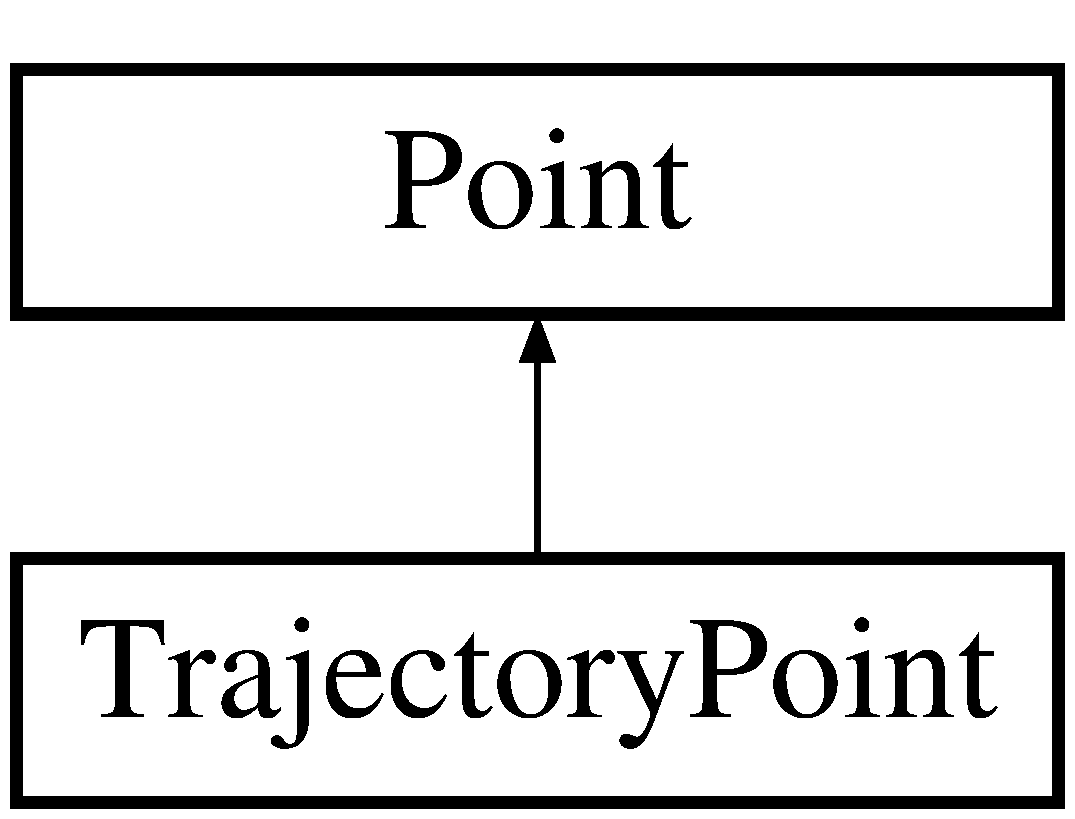
\includegraphics[height=2.000000cm]{classTrajectoryPoint}
\end{center}
\end{figure}
\subsection*{Public Member Functions}
\begin{DoxyCompactItemize}
\item 
\hyperlink{classTrajectoryPoint_a6880ea8ab699f81587357df0dff311af}{Trajectory\-Point} ()
\item 
virtual \hyperlink{classTrajectoryPoint_ab83a29f27046a0e08c8377bf7b49cf18}{$\sim$\-Trajectory\-Point} ()
\item 
void \hyperlink{classTrajectoryPoint_ae9c5623802ffa61d94a1d401a35c84a5}{set\-Position} (const \hyperlink{classMotorPosition}{Motor\-Position} \&pos)
\begin{DoxyCompactList}\small\item\em Set the position for this trajectory point. \end{DoxyCompactList}\item 
\hyperlink{classMotorPosition}{Motor\-Position} \hyperlink{classTrajectoryPoint_a6958793f5089d26b7dacc81ad5f582c2}{get\-Position} ()
\begin{DoxyCompactList}\small\item\em Get the position for this trajectory point. \end{DoxyCompactList}\item 
void \hyperlink{classTrajectoryPoint_adfe48c8c36f70ce49eb7255422c848c2}{set\-Velocity} (const \hyperlink{classMotorVelocity}{Motor\-Velocity} \&vel)
\begin{DoxyCompactList}\small\item\em Set the velocity for this trajectory point. \end{DoxyCompactList}\item 
\hyperlink{classMotorVelocity}{Motor\-Velocity} \hyperlink{classTrajectoryPoint_af51e54915c13e2e3f8c8370b1e1120c4}{get\-Velocity} ()
\begin{DoxyCompactList}\small\item\em Get the velocity for this trajectory point. \end{DoxyCompactList}\item 
void \hyperlink{classTrajectoryPoint_a27fecd9f51bc986fd19423fd91f34a47}{set\-Acceleration} (const \hyperlink{classMotorAcceleration}{Motor\-Acceleration} \&accel)
\begin{DoxyCompactList}\small\item\em Set the acceleration for this trajectory point. \end{DoxyCompactList}\item 
\hyperlink{classMotorAcceleration}{Motor\-Acceleration} \hyperlink{classTrajectoryPoint_a237388eb01ab1cc243534e42f1d365f5}{get\-Acceleration} ()
\begin{DoxyCompactList}\small\item\em Get the acceleration for this trajectory point. \end{DoxyCompactList}\item 
void \hyperlink{classTrajectoryPoint_a3f9478e0af994b1fe3258e8c31b1a26a}{set\-Duration\-M\-S} (const unsigned int duration)
\begin{DoxyCompactList}\small\item\em Set the duration for this trajectory point in milliseconds. \end{DoxyCompactList}\item 
unsigned int \hyperlink{classTrajectoryPoint_aae6bd9313448ccbc049891c934b3032d}{get\-Duration\-M\-S} ()
\begin{DoxyCompactList}\small\item\em Get the duration for this trajectory point in milliseconds. \end{DoxyCompactList}\item 
void \hyperlink{classTrajectoryPoint_a3e02eb8dae0e8f27e9f0b3c18043c0eb}{set\-Step} (const unsigned int step\-Count)
\begin{DoxyCompactList}\small\item\em Set the step count for this trajectory point. \end{DoxyCompactList}\item 
unsigned int \hyperlink{classTrajectoryPoint_a296829f5eae5f461d21ba58d7ce9391b}{get\-Step} ()
\begin{DoxyCompactList}\small\item\em Get the step count for this trajectory point. \end{DoxyCompactList}\item 
void \hyperlink{classTrajectoryPoint_a696622132c87b2be1f7dde5985d26dfc}{set\-Time\-S} (const double time)
\begin{DoxyCompactList}\small\item\em Set the relative time for this trajectory point in seconds. \end{DoxyCompactList}\item 
double \hyperlink{classTrajectoryPoint_aa17ef1030899d70b96603f758063a00b}{get\-Time\-S} ()
\begin{DoxyCompactList}\small\item\em Get the relative time for this trajectory point in seconds. \end{DoxyCompactList}\item 
void \hyperlink{classTrajectoryPoint_aeb7e7d54d48f10cd7a92411cdbbd6f91}{set\-Filter1\-Sum} (const double sum)
\begin{DoxyCompactList}\small\item\em Set the Filter 1 sum for this trajectory point. \end{DoxyCompactList}\item 
double \hyperlink{classTrajectoryPoint_a978c0ae5481d1c91374e225076b9625b}{get\-Filter1\-Sum} ()
\begin{DoxyCompactList}\small\item\em Get the Filter 1 sum for this trajectory point. \end{DoxyCompactList}\item 
void \hyperlink{classTrajectoryPoint_a6284a1c19021694a03c82436a9bef822}{set\-Filter2\-Sum} (const double sum)
\begin{DoxyCompactList}\small\item\em Set the Filter 2 sum for this trajectory point. \end{DoxyCompactList}\item 
double \hyperlink{classTrajectoryPoint_a6d81a631ced4ff5d73434c6c0e0adeaf}{get\-Filter2\-Sum} ()
\begin{DoxyCompactList}\small\item\em Get the Filter 2 sum for this trajectory point. \end{DoxyCompactList}\item 
void \hyperlink{classTrajectoryPoint_ae74248e33ae5355bebd7ba894dfddc36}{show} ()
\begin{DoxyCompactList}\small\item\em Show the trajectory point on standard output. \end{DoxyCompactList}\item 
void \hyperlink{classTrajectoryPoint_a168f92496430009453c052e042803aa8}{output\-C\-S\-V} (std\-::ofstream \&file\-C\-S\-V)
\begin{DoxyCompactList}\small\item\em Output the trajectory point to a comma-\/separated value file. \end{DoxyCompactList}\item 
void \hyperlink{classTrajectoryPoint_a8063a1ca05dd41d3df6299b51147a998}{output\-C\-S\-Vheader} (std\-::ofstream \&file\-C\-S\-V)
\begin{DoxyCompactList}\small\item\em Output the trajectory point header to a comma-\/separated value file. \end{DoxyCompactList}\end{DoxyCompactItemize}
\subsection*{Private Attributes}
\begin{DoxyCompactItemize}
\item 
\hyperlink{classMotorPosition}{Motor\-Position} \hyperlink{classTrajectoryPoint_a786f988c05632066d9759cf23c1b1ddf}{position}
\item 
\hyperlink{classMotorVelocity}{Motor\-Velocity} \hyperlink{classTrajectoryPoint_ab8782cac9ee57c49096bd94611b4d2d2}{velocity}
\item 
\hyperlink{classMotorAcceleration}{Motor\-Acceleration} \hyperlink{classTrajectoryPoint_a7633f742dd289ebbcfe09286b3840d96}{acceleration}
\item 
unsigned int \hyperlink{classTrajectoryPoint_a7e6ba8249d02b309129ea6f190ff296f}{duration\-M\-S}
\item 
unsigned int \hyperlink{classTrajectoryPoint_a11f7fb0c8a2742c89c761bc807ec6b2e}{step}
\item 
double \hyperlink{classTrajectoryPoint_a25fe1578e301cba61b31921ec98f7349}{time\-S}
\item 
double \hyperlink{classTrajectoryPoint_a98e19176c99793e4fa45f6d117878ed0}{filter1\-Sum}
\item 
double \hyperlink{classTrajectoryPoint_a384166e1e0967cdc00572418826799db}{filter2\-Sum}
\end{DoxyCompactItemize}
\subsection*{Additional Inherited Members}


\subsection{Detailed Description}
A trajectory point is a point with added velocity and duration. 

\subsection{Constructor \& Destructor Documentation}
\hypertarget{classTrajectoryPoint_a6880ea8ab699f81587357df0dff311af}{\index{Trajectory\-Point@{Trajectory\-Point}!Trajectory\-Point@{Trajectory\-Point}}
\index{Trajectory\-Point@{Trajectory\-Point}!TrajectoryPoint@{Trajectory\-Point}}
\subsubsection[{Trajectory\-Point}]{\setlength{\rightskip}{0pt plus 5cm}Trajectory\-Point\-::\-Trajectory\-Point (
\begin{DoxyParamCaption}
{}
\end{DoxyParamCaption}
)}}\label{classTrajectoryPoint_a6880ea8ab699f81587357df0dff311af}
\hypertarget{classTrajectoryPoint_ab83a29f27046a0e08c8377bf7b49cf18}{\index{Trajectory\-Point@{Trajectory\-Point}!$\sim$\-Trajectory\-Point@{$\sim$\-Trajectory\-Point}}
\index{$\sim$\-Trajectory\-Point@{$\sim$\-Trajectory\-Point}!TrajectoryPoint@{Trajectory\-Point}}
\subsubsection[{$\sim$\-Trajectory\-Point}]{\setlength{\rightskip}{0pt plus 5cm}Trajectory\-Point\-::$\sim$\-Trajectory\-Point (
\begin{DoxyParamCaption}
{}
\end{DoxyParamCaption}
)\hspace{0.3cm}{\ttfamily [virtual]}}}\label{classTrajectoryPoint_ab83a29f27046a0e08c8377bf7b49cf18}


\subsection{Member Function Documentation}
\hypertarget{classTrajectoryPoint_a237388eb01ab1cc243534e42f1d365f5}{\index{Trajectory\-Point@{Trajectory\-Point}!get\-Acceleration@{get\-Acceleration}}
\index{get\-Acceleration@{get\-Acceleration}!TrajectoryPoint@{Trajectory\-Point}}
\subsubsection[{get\-Acceleration}]{\setlength{\rightskip}{0pt plus 5cm}{\bf Motor\-Acceleration} Trajectory\-Point\-::get\-Acceleration (
\begin{DoxyParamCaption}
{}
\end{DoxyParamCaption}
)}}\label{classTrajectoryPoint_a237388eb01ab1cc243534e42f1d365f5}


Get the acceleration for this trajectory point. 

\begin{DoxyReturn}{Returns}
a \hyperlink{classMotorAcceleration}{Motor\-Acceleration} representing this trajectory points acceleration 
\end{DoxyReturn}
\hypertarget{classTrajectoryPoint_aae6bd9313448ccbc049891c934b3032d}{\index{Trajectory\-Point@{Trajectory\-Point}!get\-Duration\-M\-S@{get\-Duration\-M\-S}}
\index{get\-Duration\-M\-S@{get\-Duration\-M\-S}!TrajectoryPoint@{Trajectory\-Point}}
\subsubsection[{get\-Duration\-M\-S}]{\setlength{\rightskip}{0pt plus 5cm}unsigned int Trajectory\-Point\-::get\-Duration\-M\-S (
\begin{DoxyParamCaption}
{}
\end{DoxyParamCaption}
)}}\label{classTrajectoryPoint_aae6bd9313448ccbc049891c934b3032d}


Get the duration for this trajectory point in milliseconds. 

\begin{DoxyReturn}{Returns}
int duration in milliseconds 
\end{DoxyReturn}
\hypertarget{classTrajectoryPoint_a978c0ae5481d1c91374e225076b9625b}{\index{Trajectory\-Point@{Trajectory\-Point}!get\-Filter1\-Sum@{get\-Filter1\-Sum}}
\index{get\-Filter1\-Sum@{get\-Filter1\-Sum}!TrajectoryPoint@{Trajectory\-Point}}
\subsubsection[{get\-Filter1\-Sum}]{\setlength{\rightskip}{0pt plus 5cm}double Trajectory\-Point\-::get\-Filter1\-Sum (
\begin{DoxyParamCaption}
{}
\end{DoxyParamCaption}
)}}\label{classTrajectoryPoint_a978c0ae5481d1c91374e225076b9625b}


Get the Filter 1 sum for this trajectory point. 

\begin{DoxyReturn}{Returns}
double sum value for the Filter 1 sum 
\end{DoxyReturn}
\hypertarget{classTrajectoryPoint_a6d81a631ced4ff5d73434c6c0e0adeaf}{\index{Trajectory\-Point@{Trajectory\-Point}!get\-Filter2\-Sum@{get\-Filter2\-Sum}}
\index{get\-Filter2\-Sum@{get\-Filter2\-Sum}!TrajectoryPoint@{Trajectory\-Point}}
\subsubsection[{get\-Filter2\-Sum}]{\setlength{\rightskip}{0pt plus 5cm}double Trajectory\-Point\-::get\-Filter2\-Sum (
\begin{DoxyParamCaption}
{}
\end{DoxyParamCaption}
)}}\label{classTrajectoryPoint_a6d81a631ced4ff5d73434c6c0e0adeaf}


Get the Filter 2 sum for this trajectory point. 

\begin{DoxyReturn}{Returns}
double sum value for the Filter 2 sum 
\end{DoxyReturn}
\hypertarget{classTrajectoryPoint_a6958793f5089d26b7dacc81ad5f582c2}{\index{Trajectory\-Point@{Trajectory\-Point}!get\-Position@{get\-Position}}
\index{get\-Position@{get\-Position}!TrajectoryPoint@{Trajectory\-Point}}
\subsubsection[{get\-Position}]{\setlength{\rightskip}{0pt plus 5cm}{\bf Motor\-Position} Trajectory\-Point\-::get\-Position (
\begin{DoxyParamCaption}
{}
\end{DoxyParamCaption}
)}}\label{classTrajectoryPoint_a6958793f5089d26b7dacc81ad5f582c2}


Get the position for this trajectory point. 

\begin{DoxyReturn}{Returns}
a \hyperlink{classMotorPosition}{Motor\-Position} representing this trajectory points position 
\end{DoxyReturn}
\hypertarget{classTrajectoryPoint_a296829f5eae5f461d21ba58d7ce9391b}{\index{Trajectory\-Point@{Trajectory\-Point}!get\-Step@{get\-Step}}
\index{get\-Step@{get\-Step}!TrajectoryPoint@{Trajectory\-Point}}
\subsubsection[{get\-Step}]{\setlength{\rightskip}{0pt plus 5cm}unsigned int Trajectory\-Point\-::get\-Step (
\begin{DoxyParamCaption}
{}
\end{DoxyParamCaption}
)}}\label{classTrajectoryPoint_a296829f5eae5f461d21ba58d7ce9391b}


Get the step count for this trajectory point. 

\begin{DoxyReturn}{Returns}
unsigned int step count 
\end{DoxyReturn}
\hypertarget{classTrajectoryPoint_aa17ef1030899d70b96603f758063a00b}{\index{Trajectory\-Point@{Trajectory\-Point}!get\-Time\-S@{get\-Time\-S}}
\index{get\-Time\-S@{get\-Time\-S}!TrajectoryPoint@{Trajectory\-Point}}
\subsubsection[{get\-Time\-S}]{\setlength{\rightskip}{0pt plus 5cm}double Trajectory\-Point\-::get\-Time\-S (
\begin{DoxyParamCaption}
{}
\end{DoxyParamCaption}
)}}\label{classTrajectoryPoint_aa17ef1030899d70b96603f758063a00b}


Get the relative time for this trajectory point in seconds. 

\begin{DoxyReturn}{Returns}
double relative time in seconds 
\end{DoxyReturn}
\hypertarget{classTrajectoryPoint_af51e54915c13e2e3f8c8370b1e1120c4}{\index{Trajectory\-Point@{Trajectory\-Point}!get\-Velocity@{get\-Velocity}}
\index{get\-Velocity@{get\-Velocity}!TrajectoryPoint@{Trajectory\-Point}}
\subsubsection[{get\-Velocity}]{\setlength{\rightskip}{0pt plus 5cm}{\bf Motor\-Velocity} Trajectory\-Point\-::get\-Velocity (
\begin{DoxyParamCaption}
{}
\end{DoxyParamCaption}
)}}\label{classTrajectoryPoint_af51e54915c13e2e3f8c8370b1e1120c4}


Get the velocity for this trajectory point. 

\begin{DoxyReturn}{Returns}
a \hyperlink{classMotorVelocity}{Motor\-Velocity} representing this trajectory points velocity 
\end{DoxyReturn}
\hypertarget{classTrajectoryPoint_a168f92496430009453c052e042803aa8}{\index{Trajectory\-Point@{Trajectory\-Point}!output\-C\-S\-V@{output\-C\-S\-V}}
\index{output\-C\-S\-V@{output\-C\-S\-V}!TrajectoryPoint@{Trajectory\-Point}}
\subsubsection[{output\-C\-S\-V}]{\setlength{\rightskip}{0pt plus 5cm}void Trajectory\-Point\-::output\-C\-S\-V (
\begin{DoxyParamCaption}
\item[{std\-::ofstream \&}]{file\-C\-S\-V}
\end{DoxyParamCaption}
)}}\label{classTrajectoryPoint_a168f92496430009453c052e042803aa8}


Output the trajectory point to a comma-\/separated value file. 

\hypertarget{classTrajectoryPoint_a8063a1ca05dd41d3df6299b51147a998}{\index{Trajectory\-Point@{Trajectory\-Point}!output\-C\-S\-Vheader@{output\-C\-S\-Vheader}}
\index{output\-C\-S\-Vheader@{output\-C\-S\-Vheader}!TrajectoryPoint@{Trajectory\-Point}}
\subsubsection[{output\-C\-S\-Vheader}]{\setlength{\rightskip}{0pt plus 5cm}void Trajectory\-Point\-::output\-C\-S\-Vheader (
\begin{DoxyParamCaption}
\item[{std\-::ofstream \&}]{file\-C\-S\-V}
\end{DoxyParamCaption}
)}}\label{classTrajectoryPoint_a8063a1ca05dd41d3df6299b51147a998}


Output the trajectory point header to a comma-\/separated value file. 

\hypertarget{classTrajectoryPoint_a27fecd9f51bc986fd19423fd91f34a47}{\index{Trajectory\-Point@{Trajectory\-Point}!set\-Acceleration@{set\-Acceleration}}
\index{set\-Acceleration@{set\-Acceleration}!TrajectoryPoint@{Trajectory\-Point}}
\subsubsection[{set\-Acceleration}]{\setlength{\rightskip}{0pt plus 5cm}void Trajectory\-Point\-::set\-Acceleration (
\begin{DoxyParamCaption}
\item[{const {\bf Motor\-Acceleration} \&}]{accel}
\end{DoxyParamCaption}
)}}\label{classTrajectoryPoint_a27fecd9f51bc986fd19423fd91f34a47}


Set the acceleration for this trajectory point. 


\begin{DoxyParams}[1]{Parameters}
\mbox{\tt in}  & {\em a} & \hyperlink{classMotorAcceleration}{Motor\-Acceleration} acceleration setting \\
\hline
\end{DoxyParams}
\hypertarget{classTrajectoryPoint_a3f9478e0af994b1fe3258e8c31b1a26a}{\index{Trajectory\-Point@{Trajectory\-Point}!set\-Duration\-M\-S@{set\-Duration\-M\-S}}
\index{set\-Duration\-M\-S@{set\-Duration\-M\-S}!TrajectoryPoint@{Trajectory\-Point}}
\subsubsection[{set\-Duration\-M\-S}]{\setlength{\rightskip}{0pt plus 5cm}void Trajectory\-Point\-::set\-Duration\-M\-S (
\begin{DoxyParamCaption}
\item[{const unsigned int}]{duration}
\end{DoxyParamCaption}
)}}\label{classTrajectoryPoint_a3f9478e0af994b1fe3258e8c31b1a26a}


Set the duration for this trajectory point in milliseconds. 


\begin{DoxyParams}[1]{Parameters}
\mbox{\tt in}  & {\em int} & duration in milliseconds \\
\hline
\end{DoxyParams}
\hypertarget{classTrajectoryPoint_aeb7e7d54d48f10cd7a92411cdbbd6f91}{\index{Trajectory\-Point@{Trajectory\-Point}!set\-Filter1\-Sum@{set\-Filter1\-Sum}}
\index{set\-Filter1\-Sum@{set\-Filter1\-Sum}!TrajectoryPoint@{Trajectory\-Point}}
\subsubsection[{set\-Filter1\-Sum}]{\setlength{\rightskip}{0pt plus 5cm}void Trajectory\-Point\-::set\-Filter1\-Sum (
\begin{DoxyParamCaption}
\item[{const double}]{sum}
\end{DoxyParamCaption}
)}}\label{classTrajectoryPoint_aeb7e7d54d48f10cd7a92411cdbbd6f91}


Set the Filter 1 sum for this trajectory point. 


\begin{DoxyParams}[1]{Parameters}
\mbox{\tt in}  & {\em double} & sum value for the Filter 1 sum \\
\hline
\end{DoxyParams}
\hypertarget{classTrajectoryPoint_a6284a1c19021694a03c82436a9bef822}{\index{Trajectory\-Point@{Trajectory\-Point}!set\-Filter2\-Sum@{set\-Filter2\-Sum}}
\index{set\-Filter2\-Sum@{set\-Filter2\-Sum}!TrajectoryPoint@{Trajectory\-Point}}
\subsubsection[{set\-Filter2\-Sum}]{\setlength{\rightskip}{0pt plus 5cm}void Trajectory\-Point\-::set\-Filter2\-Sum (
\begin{DoxyParamCaption}
\item[{const double}]{sum}
\end{DoxyParamCaption}
)}}\label{classTrajectoryPoint_a6284a1c19021694a03c82436a9bef822}


Set the Filter 2 sum for this trajectory point. 


\begin{DoxyParams}[1]{Parameters}
\mbox{\tt in}  & {\em double} & sum value for the Filter 2 sum \\
\hline
\end{DoxyParams}
\hypertarget{classTrajectoryPoint_ae9c5623802ffa61d94a1d401a35c84a5}{\index{Trajectory\-Point@{Trajectory\-Point}!set\-Position@{set\-Position}}
\index{set\-Position@{set\-Position}!TrajectoryPoint@{Trajectory\-Point}}
\subsubsection[{set\-Position}]{\setlength{\rightskip}{0pt plus 5cm}void Trajectory\-Point\-::set\-Position (
\begin{DoxyParamCaption}
\item[{const {\bf Motor\-Position} \&}]{pos}
\end{DoxyParamCaption}
)}}\label{classTrajectoryPoint_ae9c5623802ffa61d94a1d401a35c84a5}


Set the position for this trajectory point. 


\begin{DoxyParams}[1]{Parameters}
\mbox{\tt in}  & {\em a} & \hyperlink{classMotorPosition}{Motor\-Position} position setting \\
\hline
\end{DoxyParams}
\hypertarget{classTrajectoryPoint_a3e02eb8dae0e8f27e9f0b3c18043c0eb}{\index{Trajectory\-Point@{Trajectory\-Point}!set\-Step@{set\-Step}}
\index{set\-Step@{set\-Step}!TrajectoryPoint@{Trajectory\-Point}}
\subsubsection[{set\-Step}]{\setlength{\rightskip}{0pt plus 5cm}void Trajectory\-Point\-::set\-Step (
\begin{DoxyParamCaption}
\item[{const unsigned int}]{step\-Count}
\end{DoxyParamCaption}
)}}\label{classTrajectoryPoint_a3e02eb8dae0e8f27e9f0b3c18043c0eb}


Set the step count for this trajectory point. 


\begin{DoxyParams}[1]{Parameters}
\mbox{\tt in}  & {\em unsigned} & int step count \\
\hline
\end{DoxyParams}
\hypertarget{classTrajectoryPoint_a696622132c87b2be1f7dde5985d26dfc}{\index{Trajectory\-Point@{Trajectory\-Point}!set\-Time\-S@{set\-Time\-S}}
\index{set\-Time\-S@{set\-Time\-S}!TrajectoryPoint@{Trajectory\-Point}}
\subsubsection[{set\-Time\-S}]{\setlength{\rightskip}{0pt plus 5cm}void Trajectory\-Point\-::set\-Time\-S (
\begin{DoxyParamCaption}
\item[{const double}]{time}
\end{DoxyParamCaption}
)}}\label{classTrajectoryPoint_a696622132c87b2be1f7dde5985d26dfc}


Set the relative time for this trajectory point in seconds. 


\begin{DoxyParams}[1]{Parameters}
\mbox{\tt in}  & {\em double} & relative in seconds \\
\hline
\end{DoxyParams}
\hypertarget{classTrajectoryPoint_adfe48c8c36f70ce49eb7255422c848c2}{\index{Trajectory\-Point@{Trajectory\-Point}!set\-Velocity@{set\-Velocity}}
\index{set\-Velocity@{set\-Velocity}!TrajectoryPoint@{Trajectory\-Point}}
\subsubsection[{set\-Velocity}]{\setlength{\rightskip}{0pt plus 5cm}void Trajectory\-Point\-::set\-Velocity (
\begin{DoxyParamCaption}
\item[{const {\bf Motor\-Velocity} \&}]{vel}
\end{DoxyParamCaption}
)}}\label{classTrajectoryPoint_adfe48c8c36f70ce49eb7255422c848c2}


Set the velocity for this trajectory point. 


\begin{DoxyParams}[1]{Parameters}
\mbox{\tt in}  & {\em a} & \hyperlink{classMotorVelocity}{Motor\-Velocity} velocity setting \\
\hline
\end{DoxyParams}
\hypertarget{classTrajectoryPoint_ae74248e33ae5355bebd7ba894dfddc36}{\index{Trajectory\-Point@{Trajectory\-Point}!show@{show}}
\index{show@{show}!TrajectoryPoint@{Trajectory\-Point}}
\subsubsection[{show}]{\setlength{\rightskip}{0pt plus 5cm}void Trajectory\-Point\-::show (
\begin{DoxyParamCaption}
{}
\end{DoxyParamCaption}
)}}\label{classTrajectoryPoint_ae74248e33ae5355bebd7ba894dfddc36}


Show the trajectory point on standard output. 



\subsection{Member Data Documentation}
\hypertarget{classTrajectoryPoint_a7633f742dd289ebbcfe09286b3840d96}{\index{Trajectory\-Point@{Trajectory\-Point}!acceleration@{acceleration}}
\index{acceleration@{acceleration}!TrajectoryPoint@{Trajectory\-Point}}
\subsubsection[{acceleration}]{\setlength{\rightskip}{0pt plus 5cm}{\bf Motor\-Acceleration} Trajectory\-Point\-::acceleration\hspace{0.3cm}{\ttfamily [private]}}}\label{classTrajectoryPoint_a7633f742dd289ebbcfe09286b3840d96}
\hypertarget{classTrajectoryPoint_a7e6ba8249d02b309129ea6f190ff296f}{\index{Trajectory\-Point@{Trajectory\-Point}!duration\-M\-S@{duration\-M\-S}}
\index{duration\-M\-S@{duration\-M\-S}!TrajectoryPoint@{Trajectory\-Point}}
\subsubsection[{duration\-M\-S}]{\setlength{\rightskip}{0pt plus 5cm}unsigned int Trajectory\-Point\-::duration\-M\-S\hspace{0.3cm}{\ttfamily [private]}}}\label{classTrajectoryPoint_a7e6ba8249d02b309129ea6f190ff296f}
\hypertarget{classTrajectoryPoint_a98e19176c99793e4fa45f6d117878ed0}{\index{Trajectory\-Point@{Trajectory\-Point}!filter1\-Sum@{filter1\-Sum}}
\index{filter1\-Sum@{filter1\-Sum}!TrajectoryPoint@{Trajectory\-Point}}
\subsubsection[{filter1\-Sum}]{\setlength{\rightskip}{0pt plus 5cm}double Trajectory\-Point\-::filter1\-Sum\hspace{0.3cm}{\ttfamily [private]}}}\label{classTrajectoryPoint_a98e19176c99793e4fa45f6d117878ed0}
\hypertarget{classTrajectoryPoint_a384166e1e0967cdc00572418826799db}{\index{Trajectory\-Point@{Trajectory\-Point}!filter2\-Sum@{filter2\-Sum}}
\index{filter2\-Sum@{filter2\-Sum}!TrajectoryPoint@{Trajectory\-Point}}
\subsubsection[{filter2\-Sum}]{\setlength{\rightskip}{0pt plus 5cm}double Trajectory\-Point\-::filter2\-Sum\hspace{0.3cm}{\ttfamily [private]}}}\label{classTrajectoryPoint_a384166e1e0967cdc00572418826799db}
\hypertarget{classTrajectoryPoint_a786f988c05632066d9759cf23c1b1ddf}{\index{Trajectory\-Point@{Trajectory\-Point}!position@{position}}
\index{position@{position}!TrajectoryPoint@{Trajectory\-Point}}
\subsubsection[{position}]{\setlength{\rightskip}{0pt plus 5cm}{\bf Motor\-Position} Trajectory\-Point\-::position\hspace{0.3cm}{\ttfamily [private]}}}\label{classTrajectoryPoint_a786f988c05632066d9759cf23c1b1ddf}
\hypertarget{classTrajectoryPoint_a11f7fb0c8a2742c89c761bc807ec6b2e}{\index{Trajectory\-Point@{Trajectory\-Point}!step@{step}}
\index{step@{step}!TrajectoryPoint@{Trajectory\-Point}}
\subsubsection[{step}]{\setlength{\rightskip}{0pt plus 5cm}unsigned int Trajectory\-Point\-::step\hspace{0.3cm}{\ttfamily [private]}}}\label{classTrajectoryPoint_a11f7fb0c8a2742c89c761bc807ec6b2e}
\hypertarget{classTrajectoryPoint_a25fe1578e301cba61b31921ec98f7349}{\index{Trajectory\-Point@{Trajectory\-Point}!time\-S@{time\-S}}
\index{time\-S@{time\-S}!TrajectoryPoint@{Trajectory\-Point}}
\subsubsection[{time\-S}]{\setlength{\rightskip}{0pt plus 5cm}double Trajectory\-Point\-::time\-S\hspace{0.3cm}{\ttfamily [private]}}}\label{classTrajectoryPoint_a25fe1578e301cba61b31921ec98f7349}
\hypertarget{classTrajectoryPoint_ab8782cac9ee57c49096bd94611b4d2d2}{\index{Trajectory\-Point@{Trajectory\-Point}!velocity@{velocity}}
\index{velocity@{velocity}!TrajectoryPoint@{Trajectory\-Point}}
\subsubsection[{velocity}]{\setlength{\rightskip}{0pt plus 5cm}{\bf Motor\-Velocity} Trajectory\-Point\-::velocity\hspace{0.3cm}{\ttfamily [private]}}}\label{classTrajectoryPoint_ab8782cac9ee57c49096bd94611b4d2d2}


The documentation for this class was generated from the following files\-:\begin{DoxyCompactItemize}
\item 
framework/\hyperlink{TrajectoryPoint_8hpp}{Trajectory\-Point.\-hpp}\item 
framework/\hyperlink{TrajectoryPoint_8cpp}{Trajectory\-Point.\-cpp}\end{DoxyCompactItemize}

\hypertarget{classWayPoint}{\section{Way\-Point Class Reference}
\label{classWayPoint}\index{Way\-Point@{Way\-Point}}
}


A waypoint is simply a point.  




{\ttfamily \#include $<$Way\-Point.\-hpp$>$}

Inheritance diagram for Way\-Point\-:\begin{figure}[H]
\begin{center}
\leavevmode
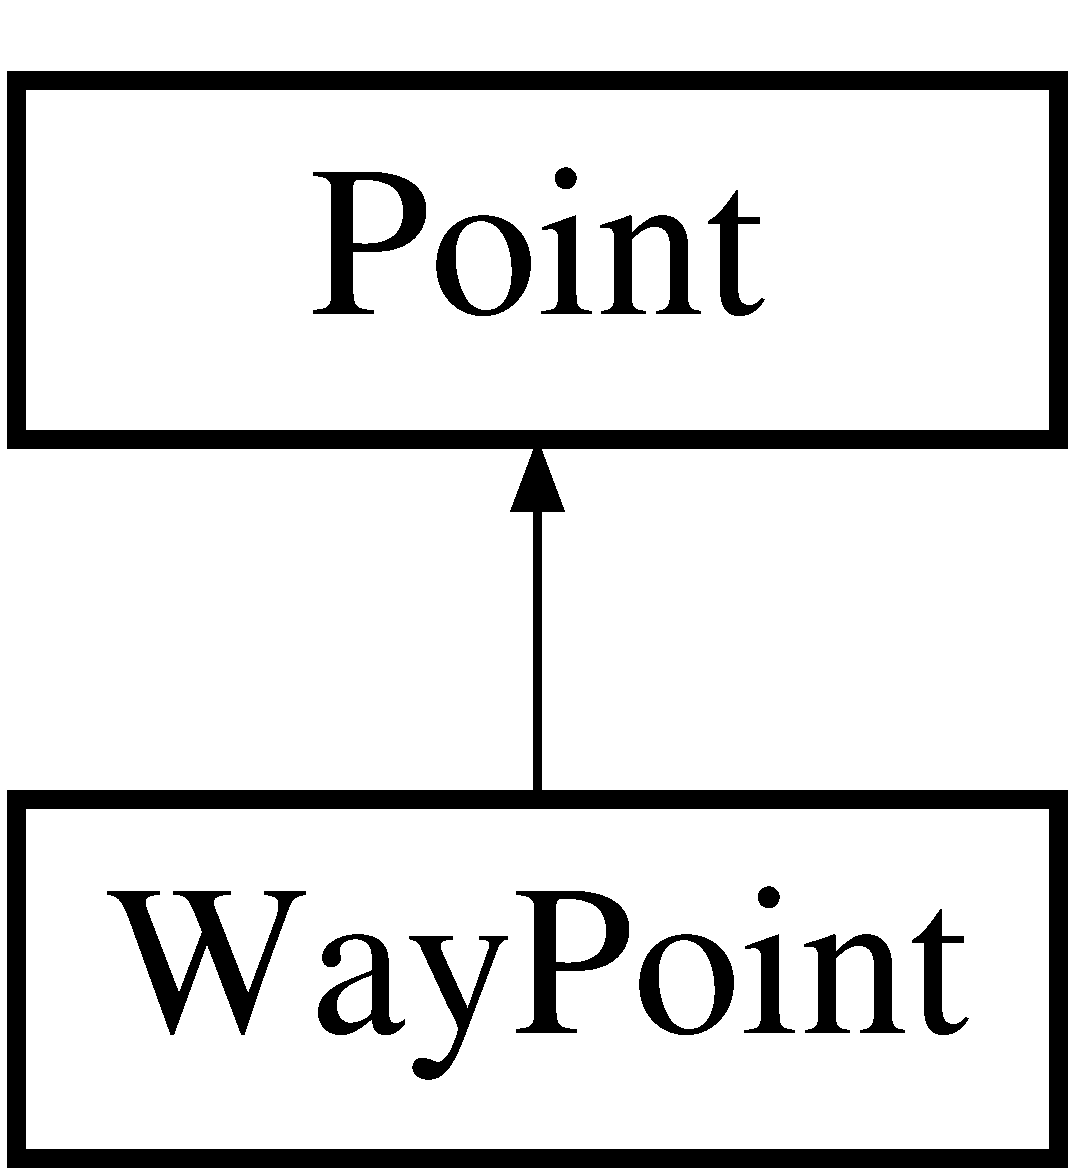
\includegraphics[height=2.000000cm]{classWayPoint}
\end{center}
\end{figure}
\subsection*{Public Member Functions}
\begin{DoxyCompactItemize}
\item 
\hyperlink{classWayPoint_a0388a615719454d38b5a8160d8058550}{Way\-Point} ()
\item 
virtual \hyperlink{classWayPoint_acb5d912197e2371772213fe2e1723316}{$\sim$\-Way\-Point} ()
\end{DoxyCompactItemize}
\subsection*{Additional Inherited Members}


\subsection{Detailed Description}
A waypoint is simply a point. 

\subsection{Constructor \& Destructor Documentation}
\hypertarget{classWayPoint_a0388a615719454d38b5a8160d8058550}{\index{Way\-Point@{Way\-Point}!Way\-Point@{Way\-Point}}
\index{Way\-Point@{Way\-Point}!WayPoint@{Way\-Point}}
\subsubsection[{Way\-Point}]{\setlength{\rightskip}{0pt plus 5cm}Way\-Point\-::\-Way\-Point (
\begin{DoxyParamCaption}
{}
\end{DoxyParamCaption}
)}}\label{classWayPoint_a0388a615719454d38b5a8160d8058550}
\hypertarget{classWayPoint_acb5d912197e2371772213fe2e1723316}{\index{Way\-Point@{Way\-Point}!$\sim$\-Way\-Point@{$\sim$\-Way\-Point}}
\index{$\sim$\-Way\-Point@{$\sim$\-Way\-Point}!WayPoint@{Way\-Point}}
\subsubsection[{$\sim$\-Way\-Point}]{\setlength{\rightskip}{0pt plus 5cm}Way\-Point\-::$\sim$\-Way\-Point (
\begin{DoxyParamCaption}
{}
\end{DoxyParamCaption}
)\hspace{0.3cm}{\ttfamily [virtual]}}}\label{classWayPoint_acb5d912197e2371772213fe2e1723316}


The documentation for this class was generated from the following files\-:\begin{DoxyCompactItemize}
\item 
framework/\hyperlink{WayPoint_8hpp}{Way\-Point.\-hpp}\item 
framework/\hyperlink{WayPoint_8cpp}{Way\-Point.\-cpp}\end{DoxyCompactItemize}

\chapter{File Documentation}
\hypertarget{main-evo1_8cpp}{\section{app/main-\/evo1.cpp File Reference}
\label{main-evo1_8cpp}\index{app/main-\/evo1.\-cpp@{app/main-\/evo1.\-cpp}}
}


A main program to drive the M\-C\-S\-F system to verify its trajectory generation capabilities.  


{\ttfamily \#include $<$iostream$>$}\\*
{\ttfamily \#include \char`\"{}../framework/\-Chassis\-Acceleration.\-hpp\char`\"{}}\\*
{\ttfamily \#include \char`\"{}../framework/\-Chassis\-Velocity.\-hpp\char`\"{}}\\*
{\ttfamily \#include \char`\"{}../framework/\-Motor\-Acceleration.\-hpp\char`\"{}}\\*
{\ttfamily \#include \char`\"{}../framework/\-Motor\-Position.\-hpp\char`\"{}}\\*
{\ttfamily \#include \char`\"{}../framework/\-Motor\-Velocity.\-hpp\char`\"{}}\\*
{\ttfamily \#include \char`\"{}../framework/\-Path.\-hpp\char`\"{}}\\*
{\ttfamily \#include \char`\"{}../framework/\-Path\-Point.\-hpp\char`\"{}}\\*
{\ttfamily \#include \char`\"{}../framework/\-Route.\-hpp\char`\"{}}\\*
{\ttfamily \#include \char`\"{}../framework/\-Trajectory.\-hpp\char`\"{}}\\*
\subsection*{Functions}
\begin{DoxyCompactItemize}
\item 
int \hyperlink{main-evo1_8cpp_ae66f6b31b5ad750f1fe042a706a4e3d4}{main} ()
\end{DoxyCompactItemize}


\subsection{Detailed Description}
A main program to drive the M\-C\-S\-F system to verify its trajectory generation capabilities. \begin{DoxyCopyright}{Copyright}
(c) 2017 Mark R. Jenkins. All rights reserved.
\end{DoxyCopyright}
\begin{DoxyAuthor}{Author}
M\-Jenkins, E\-N\-P\-M 808\-X Spring 2017 
\end{DoxyAuthor}
\begin{DoxyDate}{Date}
Mar 10, 2017 -\/ Creation
\end{DoxyDate}
This main program uses the Motion Control System Framework to generate a motion profile trajectory, then outputs the trajectory as a comma-\/separated value file in order to permit close comparison between the output of the trajectory generator in the M\-C\-S\-F and the model trajectory generator used to create the trajectory generation function in the M\-C\-S\-F. 

\subsection{Function Documentation}
\hypertarget{main-evo1_8cpp_ae66f6b31b5ad750f1fe042a706a4e3d4}{\index{main-\/evo1.\-cpp@{main-\/evo1.\-cpp}!main@{main}}
\index{main@{main}!main-evo1.cpp@{main-\/evo1.\-cpp}}
\subsubsection[{main}]{\setlength{\rightskip}{0pt plus 5cm}int main (
\begin{DoxyParamCaption}
{}
\end{DoxyParamCaption}
)}}\label{main-evo1_8cpp_ae66f6b31b5ad750f1fe042a706a4e3d4}

\hypertarget{main-evo2_8cpp}{\section{app/main-\/evo2.cpp File Reference}
\label{main-evo2_8cpp}\index{app/main-\/evo2.\-cpp@{app/main-\/evo2.\-cpp}}
}


A main program to drive the M\-C\-S\-F system to verify its trajectory generation capabilities.  


{\ttfamily \#include $<$iostream$>$}\\*
{\ttfamily \#include \char`\"{}../framework/\-Chassis.\-hpp\char`\"{}}\\*
{\ttfamily \#include \char`\"{}../framework/\-Chassis\-Acceleration.\-hpp\char`\"{}}\\*
{\ttfamily \#include \char`\"{}../framework/\-Chassis\-Turn\-Rate.\-hpp\char`\"{}}\\*
{\ttfamily \#include \char`\"{}../framework/\-Chassis\-Velocity.\-hpp\char`\"{}}\\*
{\ttfamily \#include \char`\"{}../framework/\-Drive\-System.\-hpp\char`\"{}}\\*
{\ttfamily \#include \char`\"{}../framework/\-Motor\-Acceleration.\-hpp\char`\"{}}\\*
{\ttfamily \#include \char`\"{}../framework/\-Motor\-Velocity.\-hpp\char`\"{}}\\*
{\ttfamily \#include \char`\"{}../framework/\-Path.\-hpp\char`\"{}}\\*
{\ttfamily \#include \char`\"{}../framework/\-Path\-Point.\-hpp\char`\"{}}\\*
{\ttfamily \#include \char`\"{}../framework/\-Route.\-hpp\char`\"{}}\\*
{\ttfamily \#include \char`\"{}../framework/\-Tank\-Drive.\-hpp\char`\"{}}\\*
\subsection*{Functions}
\begin{DoxyCompactItemize}
\item 
int \hyperlink{main-evo2_8cpp_ae66f6b31b5ad750f1fe042a706a4e3d4}{main} ()
\end{DoxyCompactItemize}


\subsection{Detailed Description}
A main program to drive the M\-C\-S\-F system to verify its trajectory generation capabilities. \begin{DoxyCopyright}{Copyright}
(c) 2017 Mark R. Jenkins. All rights reserved.
\end{DoxyCopyright}
\begin{DoxyAuthor}{Author}
M\-Jenkins, E\-N\-P\-M 808\-X Spring 2017 
\end{DoxyAuthor}
\begin{DoxyDate}{Date}
Mar 14, 2017 -\/ Creation
\end{DoxyDate}
This main program uses the Motion Control System Framework to generate a motion profile trajectory for a \hyperlink{classChassis}{Chassis} with a \hyperlink{classTankDrive}{Tank\-Drive}, then outputs the two trajectories (one per side of the tank drive) in order to demonstrate the ability to generate matched pairs of trajectories capable of moving a tank drive-\/based system in the desired path using motion profiling. 

\subsection{Function Documentation}
\hypertarget{main-evo2_8cpp_ae66f6b31b5ad750f1fe042a706a4e3d4}{\index{main-\/evo2.\-cpp@{main-\/evo2.\-cpp}!main@{main}}
\index{main@{main}!main-evo2.cpp@{main-\/evo2.\-cpp}}
\subsubsection[{main}]{\setlength{\rightskip}{0pt plus 5cm}int main (
\begin{DoxyParamCaption}
{}
\end{DoxyParamCaption}
)}}\label{main-evo2_8cpp_ae66f6b31b5ad750f1fe042a706a4e3d4}

\hypertarget{Chassis_8cpp}{\section{framework/\-Chassis.cpp File Reference}
\label{Chassis_8cpp}\index{framework/\-Chassis.\-cpp@{framework/\-Chassis.\-cpp}}
}


A \hyperlink{classChassis}{Chassis} has a \hyperlink{classDriveSystem}{Drive\-System} and a name, and can move using the Motion Control System Framework.  


{\ttfamily \#include \char`\"{}Chassis.\-hpp\char`\"{}}\\*


\subsection{Detailed Description}
A \hyperlink{classChassis}{Chassis} has a \hyperlink{classDriveSystem}{Drive\-System} and a name, and can move using the Motion Control System Framework. \begin{DoxyCopyright}{Copyright}
(c) 2017 Mark R. Jenkins. All rights reserved.
\end{DoxyCopyright}
\begin{DoxyAuthor}{Author}
M\-Jenkins, E\-N\-P\-M 808\-X Spring 2017 
\end{DoxyAuthor}
\begin{DoxyDate}{Date}
Mar 14, 2017 -\/ Creation
\end{DoxyDate}
The \hyperlink{classChassis}{Chassis} class represents a robot chassis. The chassis has a \hyperlink{classDriveSystem}{Drive\-System}, which can be of different types (only a \hyperlink{classTankDrive}{Tank\-Drive} is derived from the \hyperlink{classDriveSystem}{Drive\-System} class at this time). Once the \hyperlink{classDriveSystem}{Drive\-System} has been configured and set in the chassis, the chassis can be commanded to move with a distance, a turn rate (0 for straight, $<$ 0 for left turns, $>$ 0 for right turns), a velocity, and an acceleration. While operating within the constraints of the drive system (which has maximum velocity and acceleration constraints), the drive system will create a path for the motion, generate trajectories, and either execute (after customizing the execution method for a particular hardware implementation) or demonstrate the trajectories (by outputting comma-\/separated value files for the trajectories, named with the chassis name as the leading element of the C\-S\-V file name. 
\hypertarget{Chassis_8hpp}{\section{framework/\-Chassis.hpp File Reference}
\label{Chassis_8hpp}\index{framework/\-Chassis.\-hpp@{framework/\-Chassis.\-hpp}}
}


A \hyperlink{classChassis}{Chassis} has a \hyperlink{classDriveSystem}{Drive\-System} and a name, and can move using the Motion Control System Framework.  


{\ttfamily \#include $<$memory$>$}\\*
{\ttfamily \#include $<$string$>$}\\*
{\ttfamily \#include \char`\"{}Chassis\-Acceleration.\-hpp\char`\"{}}\\*
{\ttfamily \#include \char`\"{}Chassis\-Turn\-Rate.\-hpp\char`\"{}}\\*
{\ttfamily \#include \char`\"{}Chassis\-Velocity.\-hpp\char`\"{}}\\*
{\ttfamily \#include \char`\"{}Drive\-System.\-hpp\char`\"{}}\\*
{\ttfamily \#include \char`\"{}Tank\-Drive.\-hpp\char`\"{}}\\*
\subsection*{Classes}
\begin{DoxyCompactItemize}
\item 
class \hyperlink{classChassis}{Chassis}
\begin{DoxyCompactList}\small\item\em A \hyperlink{classChassis}{Chassis} has a \hyperlink{classDriveSystem}{Drive\-System} and a name, and can move using the Motion Control System Framework. \end{DoxyCompactList}\end{DoxyCompactItemize}


\subsection{Detailed Description}
A \hyperlink{classChassis}{Chassis} has a \hyperlink{classDriveSystem}{Drive\-System} and a name, and can move using the Motion Control System Framework. \begin{DoxyCopyright}{Copyright}
(c) 2017 Mark R. Jenkins. All rights reserved.
\end{DoxyCopyright}
\begin{DoxyAuthor}{Author}
M\-Jenkins, E\-N\-P\-M 808\-X Spring 2017 
\end{DoxyAuthor}
\begin{DoxyDate}{Date}
Mar 14, 2017 -\/ Creation
\end{DoxyDate}
The \hyperlink{classChassis}{Chassis} class represents a robot chassis. The chassis has a \hyperlink{classDriveSystem}{Drive\-System}, which can be of different types (only a \hyperlink{classTankDrive}{Tank\-Drive} is derived from the \hyperlink{classDriveSystem}{Drive\-System} class at this time). Once the \hyperlink{classDriveSystem}{Drive\-System} has been configured and set in the chassis, the chassis can be commanded to move with a distance, a turn rate (0 for straight, $<$ 0 for left turns, $>$ 0 for right turns), a velocity, and an acceleration. While operating within the constraints of the drive system (which has maximum velocity and acceleration constraints), the drive system will create a path for the motion, generate trajectories, and either execute (after customizing the execution method for a particular hardware implementation) or demonstrate the trajectories (by outputting comma-\/separated value files for the trajectories, named with the chassis name as the leading element of the C\-S\-V file name. 
\hypertarget{ChassisAcceleration_8cpp}{\section{framework/\-Chassis\-Acceleration.cpp File Reference}
\label{ChassisAcceleration_8cpp}\index{framework/\-Chassis\-Acceleration.\-cpp@{framework/\-Chassis\-Acceleration.\-cpp}}
}


A class to define a strict type for chassis accelerations.  


{\ttfamily \#include \char`\"{}Chassis\-Acceleration.\-hpp\char`\"{}}\\*


\subsection{Detailed Description}
A class to define a strict type for chassis accelerations. \begin{DoxyCopyright}{Copyright}
(c) 2017 Mark R. Jenkins. All rights reserved.
\end{DoxyCopyright}
\begin{DoxyAuthor}{Author}
M\-Jenkins, E\-N\-P\-M 808\-X Spring 2017 
\end{DoxyAuthor}
\begin{DoxyDate}{Date}
Mar 13, 2017 -\/ Creation
\end{DoxyDate}
\hyperlink{classChassis}{Chassis} accelerations can be specified in a variety of ways; the one chosen for initial implementation is feet per second per second. This class creates a strict type for chassis accelerations, and can provide a variety of accessor functions to allow setting/getting the acceleration in different units. The class stores the acceleration internally as \char`\"{}\-Feet Per Second Per Second\char`\"{} (fps/s). 
\hypertarget{ChassisAcceleration_8hpp}{\section{framework/\-Chassis\-Acceleration.hpp File Reference}
\label{ChassisAcceleration_8hpp}\index{framework/\-Chassis\-Acceleration.\-hpp@{framework/\-Chassis\-Acceleration.\-hpp}}
}


A class to define a strict type for chassis accelerations.  


\subsection*{Classes}
\begin{DoxyCompactItemize}
\item 
class \hyperlink{classChassisAcceleration}{Chassis\-Acceleration}
\begin{DoxyCompactList}\small\item\em Defines a strict type for chassis accelerations. \end{DoxyCompactList}\end{DoxyCompactItemize}


\subsection{Detailed Description}
A class to define a strict type for chassis accelerations. \begin{DoxyCopyright}{Copyright}
(c) 2017 Mark R. Jenkins. All rights reserved.
\end{DoxyCopyright}
\begin{DoxyAuthor}{Author}
M\-Jenkins, E\-N\-P\-M 808\-X Spring 2017 
\end{DoxyAuthor}
\begin{DoxyDate}{Date}
Mar 13, 2017 -\/ Creation
\end{DoxyDate}
\hyperlink{classChassis}{Chassis} accelerations can be specified in a variety of ways; the one chosen for initial implementation is feet per second per second. This class creates a strict type for chassis accelerations, and can provide a variety of accessor functions to allow setting/getting the acceleration in different units. The class stores the acceleration internally as \char`\"{}\-Feet Per Second Per Second\char`\"{} (fps/s). 
\hypertarget{ChassisTurnRate_8cpp}{\section{framework/\-Chassis\-Turn\-Rate.cpp File Reference}
\label{ChassisTurnRate_8cpp}\index{framework/\-Chassis\-Turn\-Rate.\-cpp@{framework/\-Chassis\-Turn\-Rate.\-cpp}}
}


\hyperlink{classChassisTurnRate}{Chassis\-Turn\-Rate} is a strictly defined type for specifying the turn rate of a moving chassis.  


{\ttfamily \#include \char`\"{}Chassis\-Turn\-Rate.\-hpp\char`\"{}}\\*


\subsection{Detailed Description}
\hyperlink{classChassisTurnRate}{Chassis\-Turn\-Rate} is a strictly defined type for specifying the turn rate of a moving chassis. \begin{DoxyCopyright}{Copyright}
(c) 2017 Mark R. Jenkins. All rights reserved.
\end{DoxyCopyright}
\begin{DoxyAuthor}{Author}
M\-Jenkins, E\-N\-P\-M 808\-X Spring 2017 
\end{DoxyAuthor}
\begin{DoxyDate}{Date}
Mar 13, 2017 -\/ Creation
\end{DoxyDate}
\hyperlink{classChassis}{Chassis} turn rates may be specified in a variety of ways; the one implemented here is as a degree of turn per foot of movement. This class creates a strict type for chassis turn rates, and can provide a variety of accessor functiont so allow setting/getting the turn rate in different units. The class stores the turn rate internaly as \char`\"{}\-Degrees per Foot of movement\char`\"{}. Note that a zero turn rate indicates movement straight ahead, a negative turn rate indicates a deviation (turn) to the left, and a positive turn rate indicates a deviation (turn) to the right. 
\hypertarget{ChassisTurnRate_8hpp}{\section{framework/\-Chassis\-Turn\-Rate.hpp File Reference}
\label{ChassisTurnRate_8hpp}\index{framework/\-Chassis\-Turn\-Rate.\-hpp@{framework/\-Chassis\-Turn\-Rate.\-hpp}}
}


\hyperlink{classChassisTurnRate}{Chassis\-Turn\-Rate} is a strictly defined type for specifying the turn rate of a moving chassis.  


\subsection*{Classes}
\begin{DoxyCompactItemize}
\item 
class \hyperlink{classChassisTurnRate}{Chassis\-Turn\-Rate}
\begin{DoxyCompactList}\small\item\em \hyperlink{classChassisTurnRate}{Chassis\-Turn\-Rate} objects are used to specify a change in direction when a chassis is moving. \end{DoxyCompactList}\end{DoxyCompactItemize}


\subsection{Detailed Description}
\hyperlink{classChassisTurnRate}{Chassis\-Turn\-Rate} is a strictly defined type for specifying the turn rate of a moving chassis. \begin{DoxyCopyright}{Copyright}
(c) 2017 Mark R. Jenkins. All rights reserved.
\end{DoxyCopyright}
\begin{DoxyAuthor}{Author}
M\-Jenkins, E\-N\-P\-M 808\-X Spring 2017 
\end{DoxyAuthor}
\begin{DoxyDate}{Date}
Mar 13, 2017 -\/ Creation
\end{DoxyDate}
\hyperlink{classChassis}{Chassis} turn rates may be specified in a variety of ways; the one implemented here is as a degree of turn per foot of movement. This class creates a strict type for chassis turn rates, and can provide a variety of accessor functiont so allow setting/getting the turn rate in different units. The class stores the turn rate internaly as \char`\"{}\-Degrees per Foot of movement\char`\"{}. Note that a zero turn rate indicates movement straight ahead, a negative turn rate indicates a deviation (turn) to the left, and a positive turn rate indicates a deviation (turn) to the right. 
\hypertarget{ChassisVelocity_8cpp}{\section{framework/\-Chassis\-Velocity.cpp File Reference}
\label{ChassisVelocity_8cpp}\index{framework/\-Chassis\-Velocity.\-cpp@{framework/\-Chassis\-Velocity.\-cpp}}
}


A class to define a strict type for chassis velocities.  


{\ttfamily \#include \char`\"{}Chassis\-Velocity.\-hpp\char`\"{}}\\*


\subsection{Detailed Description}
A class to define a strict type for chassis velocities. \begin{DoxyCopyright}{Copyright}
(c) 2017 Mark R. Jenkins. All rights reserved.
\end{DoxyCopyright}
\begin{DoxyAuthor}{Author}
M\-Jenkins, E\-N\-P\-M 808\-X Spring 2017 
\end{DoxyAuthor}
\begin{DoxyDate}{Date}
Mar 13, 2017 -\/ Creation
\end{DoxyDate}
\hyperlink{classChassis}{Chassis} velocities can be specified in a variety of ways; the one chosen for initial implementation is feet per second. This class creates a strict type for chassis velocities, and can provide a variety of accessor functions to allow setting/getting the velocity in different units. The class stores the velocity internally as \char`\"{}\-Feet Per Second\char`\"{} (fps). 
\hypertarget{ChassisVelocity_8hpp}{\section{framework/\-Chassis\-Velocity.hpp File Reference}
\label{ChassisVelocity_8hpp}\index{framework/\-Chassis\-Velocity.\-hpp@{framework/\-Chassis\-Velocity.\-hpp}}
}


A class to define a strict type for chassis velocities.  


\subsection*{Classes}
\begin{DoxyCompactItemize}
\item 
class \hyperlink{classChassisVelocity}{Chassis\-Velocity}
\begin{DoxyCompactList}\small\item\em A strictly defined type for chassis velocities. \end{DoxyCompactList}\end{DoxyCompactItemize}


\subsection{Detailed Description}
A class to define a strict type for chassis velocities. \begin{DoxyCopyright}{Copyright}
(c) 2017 Mark R. Jenkins. All rights reserved.
\end{DoxyCopyright}
\begin{DoxyAuthor}{Author}
M\-Jenkins, E\-N\-P\-M 808\-X Spring 2017 
\end{DoxyAuthor}
\begin{DoxyDate}{Date}
Mar 13, 2017 -\/ Creation
\end{DoxyDate}
\hyperlink{classChassis}{Chassis} velocities can be specified in a variety of ways; the one chosen for initial implementation is feet per second. This class creates a strict type for chassis velocities, and can provide a variety of accessor functions to allow setting/getting the velocity in different units. The class stores the velocity internally as \char`\"{}\-Feet Per Second\char`\"{} (fps). 
\hypertarget{DriveSystem_8cpp}{\section{framework/\-Drive\-System.cpp File Reference}
\label{DriveSystem_8cpp}\index{framework/\-Drive\-System.\-cpp@{framework/\-Drive\-System.\-cpp}}
}


A base class for representing drive system objects.  


{\ttfamily \#include \char`\"{}Drive\-System.\-hpp\char`\"{}}\\*


\subsection{Detailed Description}
A base class for representing drive system objects. \begin{DoxyCopyright}{Copyright}
(c) 2017 Mark R. Jenkins. All rights reserved.
\end{DoxyCopyright}
\begin{DoxyAuthor}{Author}
M\-Jenkins, E\-N\-P\-M 808\-X Spring 2017 
\end{DoxyAuthor}
\begin{DoxyDate}{Date}
Mar 13, 2017 -\/ Creation
\end{DoxyDate}
There can be many kinds of drive systems. Attributes and methods generalized from all types are implemented in this base class. The actual objects are intended to be instantiated from class defintions derived from this base class. 
\hypertarget{DriveSystem_8hpp}{\section{framework/\-Drive\-System.hpp File Reference}
\label{DriveSystem_8hpp}\index{framework/\-Drive\-System.\-hpp@{framework/\-Drive\-System.\-hpp}}
}


A base class for representing drive system objects.  


{\ttfamily \#include $<$string$>$}\\*
{\ttfamily \#include \char`\"{}Chassis\-Acceleration.\-hpp\char`\"{}}\\*
{\ttfamily \#include \char`\"{}Chassis\-Turn\-Rate.\-hpp\char`\"{}}\\*
{\ttfamily \#include \char`\"{}Chassis\-Velocity.\-hpp\char`\"{}}\\*
{\ttfamily \#include \char`\"{}Motor\-Acceleration.\-hpp\char`\"{}}\\*
{\ttfamily \#include \char`\"{}Motor\-Velocity.\-hpp\char`\"{}}\\*
\subsection*{Classes}
\begin{DoxyCompactItemize}
\item 
class \hyperlink{classDriveSystem}{Drive\-System}
\begin{DoxyCompactList}\small\item\em Base class for representing drive system objects. \end{DoxyCompactList}\end{DoxyCompactItemize}


\subsection{Detailed Description}
A base class for representing drive system objects. \begin{DoxyCopyright}{Copyright}
(c) 2017 Mark R. Jenkins. All rights reserved.
\end{DoxyCopyright}
\begin{DoxyAuthor}{Author}
M\-Jenkins, E\-N\-P\-M 808\-X Spring 2017 
\end{DoxyAuthor}
\begin{DoxyDate}{Date}
Mar 13, 2017 -\/ Creation
\end{DoxyDate}
There can be many kinds of drive systems. Attributes and methods generalized from all types are implemented in this base class. The actual objects are intended to be instantiated from class defintions derived from this base class. 
\hypertarget{MotorAcceleration_8cpp}{\section{framework/\-Motor\-Acceleration.cpp File Reference}
\label{MotorAcceleration_8cpp}\index{framework/\-Motor\-Acceleration.\-cpp@{framework/\-Motor\-Acceleration.\-cpp}}
}


A class for a strictly typed representation of motor acceleration.  


{\ttfamily \#include \char`\"{}Motor\-Acceleration.\-hpp\char`\"{}}\\*


\subsection{Detailed Description}
A class for a strictly typed representation of motor acceleration. \begin{DoxyCopyright}{Copyright}
(c) 2017 Mark R. Jenkins. All rights reserved.
\end{DoxyCopyright}
\begin{DoxyAuthor}{Author}
M\-Jenkins, E\-N\-P\-M 808\-X Spring 2017 
\end{DoxyAuthor}
\begin{DoxyDate}{Date}
Mar 5, 2017 -\/ Creation
\end{DoxyDate}
Motor accelerations can be specified in a variety of ways; a change in encoder tick rates per unit of time, or a change in motor rotation rates per unit of time are two of these. This class creates a strict type for motor accelerations, and can provide a variety of accessor functions to allow setting/getting the velocity in different units. The class stores the acceleration internally as \char`\"{}\-Rotations Per Minute per second\char`\"{} (R\-P\-M/s). 
\hypertarget{MotorAcceleration_8hpp}{\section{framework/\-Motor\-Acceleration.hpp File Reference}
\label{MotorAcceleration_8hpp}\index{framework/\-Motor\-Acceleration.\-hpp@{framework/\-Motor\-Acceleration.\-hpp}}
}


A class for a strictly typed representation of motor acceleration.  


{\ttfamily \#include \char`\"{}Chassis\-Acceleration.\-hpp\char`\"{}}\\*
\subsection*{Classes}
\begin{DoxyCompactItemize}
\item 
class \hyperlink{classMotorAcceleration}{Motor\-Acceleration}
\begin{DoxyCompactList}\small\item\em A class to provide a strict type for specifying motor acceleration. \end{DoxyCompactList}\end{DoxyCompactItemize}


\subsection{Detailed Description}
A class for a strictly typed representation of motor acceleration. \begin{DoxyCopyright}{Copyright}
(c) 2017 Mark R. Jenkins. All rights reserved.
\end{DoxyCopyright}
\begin{DoxyAuthor}{Author}
M\-Jenkins, E\-N\-P\-M 808\-X Spring 2017 
\end{DoxyAuthor}
\begin{DoxyDate}{Date}
Mar 5, 2017 -\/ Creation
\end{DoxyDate}
Motor accelerations can be specified in a variety of ways; a change in encoder tick rates per unit of time, or a change in motor rotation rates per unit of time are two of these. This class creates a strict type for motor accelerations, and can provide a variety of accessor functions to allow setting/getting the velocity in different units. The class stores the acceleration internally as \char`\"{}\-Rotations Per Minute per second\char`\"{} (R\-P\-M/s). 
\hypertarget{MotorPosition_8cpp}{\section{framework/\-Motor\-Position.cpp File Reference}
\label{MotorPosition_8cpp}\index{framework/\-Motor\-Position.\-cpp@{framework/\-Motor\-Position.\-cpp}}
}


Creates a defined type for a position based on a motor encoder.  


{\ttfamily \#include \char`\"{}Motor\-Position.\-hpp\char`\"{}}\\*


\subsection{Detailed Description}
Creates a defined type for a position based on a motor encoder. \begin{DoxyCopyright}{Copyright}
(c) 2017 Mark R. Jenkins. All rights reserved.
\end{DoxyCopyright}
\begin{DoxyAuthor}{Author}
M\-Jenkins, E\-N\-P\-M 808\-X Spring 2017 
\end{DoxyAuthor}
\begin{DoxyDate}{Date}
Mar 5, 2017 -\/ Creation 

Mar 9, 2017 -\/ Added minus operator
\begin{DoxyItemize}
\item One type of position measurement is through the value of an absolute motor encoder reading. This class creates a strictly-\/typed value to be used for such a position. 
\end{DoxyItemize}
\end{DoxyDate}

\hypertarget{MotorPosition_8hpp}{\section{framework/\-Motor\-Position.hpp File Reference}
\label{MotorPosition_8hpp}\index{framework/\-Motor\-Position.\-hpp@{framework/\-Motor\-Position.\-hpp}}
}


Creates a defined type for a position based on a motor encoder.  


\subsection*{Classes}
\begin{DoxyCompactItemize}
\item 
class \hyperlink{classMotorPosition}{Motor\-Position}
\begin{DoxyCompactList}\small\item\em Creates a defined type for a position based on a motor encoder. \end{DoxyCompactList}\end{DoxyCompactItemize}


\subsection{Detailed Description}
Creates a defined type for a position based on a motor encoder. \begin{DoxyCopyright}{Copyright}
(c) 2017 Mark R. Jenkins. All rights reserved.
\end{DoxyCopyright}
\begin{DoxyAuthor}{Author}
M\-Jenkins, E\-N\-P\-M 808\-X Spring 2017 
\end{DoxyAuthor}
\begin{DoxyDate}{Date}
Mar 5, 2017 -\/ Creation 

Mar 9, 2017 -\/ Added minus operator
\end{DoxyDate}
One type of position measurement is through the value of an absolute motor encoder reading. This class creates a strictly-\/typed value to be used for such a position. 
\hypertarget{MotorVelocity_8cpp}{\section{framework/\-Motor\-Velocity.cpp File Reference}
\label{MotorVelocity_8cpp}\index{framework/\-Motor\-Velocity.\-cpp@{framework/\-Motor\-Velocity.\-cpp}}
}


A class to define a strict type for motor velocities.  


{\ttfamily \#include \char`\"{}Motor\-Velocity.\-hpp\char`\"{}}\\*


\subsection{Detailed Description}
A class to define a strict type for motor velocities. \begin{DoxyCopyright}{Copyright}
(c) 2017 Mark R. Jenkins. All rights reserved.
\end{DoxyCopyright}
\begin{DoxyAuthor}{Author}
M\-Jenkins, E\-N\-P\-M 808\-X Spring 2017 
\end{DoxyAuthor}
\begin{DoxyDate}{Date}
Mar 5, 2017 -\/ Creation
\end{DoxyDate}
Motor velocities can be specified in a variety of ways; encoder ticks per unit of time, or motor rotations per unit of time are two of these. This class creates a strict type for motor velocities, and can provide a variety of accessor functions to allow setting/getting the velocity in different units. The class stores the velocity internally as \char`\"{}\-Rotations Per Minute\char`\"{} (R\-P\-M). 
\hypertarget{MotorVelocity_8hpp}{\section{framework/\-Motor\-Velocity.hpp File Reference}
\label{MotorVelocity_8hpp}\index{framework/\-Motor\-Velocity.\-hpp@{framework/\-Motor\-Velocity.\-hpp}}
}


A class to define a strict type for motor velocities.  


{\ttfamily \#include \char`\"{}Chassis\-Velocity.\-hpp\char`\"{}}\\*
\subsection*{Classes}
\begin{DoxyCompactItemize}
\item 
class \hyperlink{classMotorVelocity}{Motor\-Velocity}
\begin{DoxyCompactList}\small\item\em The \hyperlink{classMotorVelocity}{Motor\-Velocity} class is a strict type for motor velocities. \end{DoxyCompactList}\end{DoxyCompactItemize}


\subsection{Detailed Description}
A class to define a strict type for motor velocities. \begin{DoxyCopyright}{Copyright}
(c) 2017 Mark R. Jenkins. All rights reserved.
\end{DoxyCopyright}
\begin{DoxyAuthor}{Author}
M\-Jenkins, E\-N\-P\-M 808\-X Spring 2017 
\end{DoxyAuthor}
\begin{DoxyDate}{Date}
Mar 5, 2017 -\/ Creation
\end{DoxyDate}
Motor velocities can be specified in a variety of ways; encoder ticks per unit of time, or motor rotations per unit of time are two of these. This class creates a strict type for motor velocities, and can provide a variety of accessor functions to allow setting/getting the velocity in different units. The class stores the velocity internally as \char`\"{}\-Rotations Per Minute\char`\"{} (R\-P\-M). 
\hypertarget{Path_8cpp}{\section{framework/\-Path.cpp File Reference}
\label{Path_8cpp}\index{framework/\-Path.\-cpp@{framework/\-Path.\-cpp}}
}


A motion path is a vector of \hyperlink{classPath}{Path} Points.  


{\ttfamily \#include \char`\"{}Path.\-hpp\char`\"{}}\\*


\subsection{Detailed Description}
A motion path is a vector of \hyperlink{classPath}{Path} Points. \begin{DoxyCopyright}{Copyright}
(c) 2017 Mark R. Jenkins. All rights reserved.
\end{DoxyCopyright}
\begin{DoxyAuthor}{Author}
M\-Jenkins, E\-N\-P\-M 808\-X Spring 2017 
\end{DoxyAuthor}
\begin{DoxyDate}{Date}
Mar 6, 2017 -\/ Creation 

Mar 9, 2017 -\/ Removed plan\-Trajectory (moved to \hyperlink{classTrajectory}{Trajectory} object) 

Mar 9, 2017 -\/ Added get\-First\-Path\-Point, get\-Next\-Path\-Point, and size methods to facilitate trajectory generation from \hyperlink{classTrajectory}{Trajectory} object
\end{DoxyDate}
$\ast$\-A motion path represents a planned series of points through which a motion will travel. The path can be used to plan a motion profile trajectory. 
\hypertarget{Path_8hpp}{\section{framework/\-Path.hpp File Reference}
\label{Path_8hpp}\index{framework/\-Path.\-hpp@{framework/\-Path.\-hpp}}
}


A motion path is a vector of \hyperlink{classPath}{Path} Points.  


{\ttfamily \#include $<$iostream$>$}\\*
{\ttfamily \#include $<$vector$>$}\\*
{\ttfamily \#include \char`\"{}Path\-Point.\-hpp\char`\"{}}\\*
\subsection*{Classes}
\begin{DoxyCompactItemize}
\item 
class \hyperlink{classPath}{Path}
\begin{DoxyCompactList}\small\item\em A motion path is a series of path points between two Way Points. \end{DoxyCompactList}\end{DoxyCompactItemize}


\subsection{Detailed Description}
A motion path is a vector of \hyperlink{classPath}{Path} Points. \begin{DoxyCopyright}{Copyright}
(c) 2017 Mark R. Jenkins. All rights reserved.
\end{DoxyCopyright}
\begin{DoxyAuthor}{Author}
M\-Jenkins, E\-N\-P\-M 808\-X Spring 2017 
\end{DoxyAuthor}
\begin{DoxyDate}{Date}
Mar 6, 2017 -\/ Creation 

Mar 9, 2017 -\/ Removed plan\-Trajectory (moved to \hyperlink{classTrajectory}{Trajectory} object) 

Mar 9, 2017 -\/ Added get\-First\-Path\-Point, get\-Next\-Path\-Point, and size methods to facilitate trajectory generation from \hyperlink{classTrajectory}{Trajectory} object
\end{DoxyDate}
A motion path represents a planned series of points through which a motion will travel. The path can be used to plan a motion profile trajectory. 
\hypertarget{PathPoint_8cpp}{\section{framework/\-Path\-Point.cpp File Reference}
\label{PathPoint_8cpp}\index{framework/\-Path\-Point.\-cpp@{framework/\-Path\-Point.\-cpp}}
}


A representation of a point along a path with maximum velocity and maximum acceleration constraints.  


{\ttfamily \#include \char`\"{}Path\-Point.\-hpp\char`\"{}}\\*


\subsection{Detailed Description}
A representation of a point along a path with maximum velocity and maximum acceleration constraints. \begin{DoxyCopyright}{Copyright}
(c) 2017 Mark R. Jenkins. All rights reserved.
\end{DoxyCopyright}
\begin{DoxyAuthor}{Author}
M\-Jenkins, E\-N\-P\-M 808\-X Spring 2017 
\end{DoxyAuthor}
\begin{DoxyDate}{Date}
Mar 5, 2017 -\/ Creation
\end{DoxyDate}
A path to be used for motion profiling trajectories needs to include velocity and acceleration constraints to be used in constructing a motion profile that shapes the motion based on the maximum velocities and accelerations to be used in achieving motion. 
\hypertarget{PathPoint_8hpp}{\section{framework/\-Path\-Point.hpp File Reference}
\label{PathPoint_8hpp}\index{framework/\-Path\-Point.\-hpp@{framework/\-Path\-Point.\-hpp}}
}


A representation of a point along a path with maximum velocity and maximum acceleration constraints.  


{\ttfamily \#include $<$iostream$>$}\\*
{\ttfamily \#include \char`\"{}Motor\-Acceleration.\-hpp\char`\"{}}\\*
{\ttfamily \#include \char`\"{}Motor\-Velocity.\-hpp\char`\"{}}\\*
{\ttfamily \#include \char`\"{}Point.\-hpp\char`\"{}}\\*
\subsection*{Classes}
\begin{DoxyCompactItemize}
\item 
class \hyperlink{classPathPoint}{Path\-Point}
\begin{DoxyCompactList}\small\item\em A motion path point has a maximum velocity and acceleration for motion from this point. \end{DoxyCompactList}\end{DoxyCompactItemize}


\subsection{Detailed Description}
A representation of a point along a path with maximum velocity and maximum acceleration constraints. \begin{DoxyCopyright}{Copyright}
(c) 2017 Mark R. Jenkins. All rights reserved.
\end{DoxyCopyright}
\begin{DoxyAuthor}{Author}
M\-Jenkins, E\-N\-P\-M 808\-X Spring 2017 
\end{DoxyAuthor}
\begin{DoxyDate}{Date}
Mar 5, 2017 -\/ Creation
\end{DoxyDate}
A path to be used for motion profiling trajectories needs to include velocity and acceleration constraints to be used in constructing a motion profile that shapes the motion based on the maximum velocities and accelerations to be used in achieving motion. 
\hypertarget{Point_8cpp}{\section{framework/\-Point.cpp File Reference}
\label{Point_8cpp}\index{framework/\-Point.\-cpp@{framework/\-Point.\-cpp}}
}


A base class to define common members of \hyperlink{classPoint}{Point} objects.  


{\ttfamily \#include \char`\"{}Point.\-hpp\char`\"{}}\\*


\subsection{Detailed Description}
A base class to define common members of \hyperlink{classPoint}{Point} objects. \begin{DoxyCopyright}{Copyright}
(c) 2017 Mark R. Jenkins. All rights reserved.
\end{DoxyCopyright}
\begin{DoxyAuthor}{Author}
M\-Jenkins, E\-N\-P\-M 808\-X Spring 2017 
\end{DoxyAuthor}
\begin{DoxyDate}{Date}
Mar 5, 2017 -\/ Creation
\end{DoxyDate}
There are at least three types of \hyperlink{classPoint}{Point} objects -\/ Way\-Points, Path\-Points, and Trajectory\-Points. All three have in common a position with accessor methods to set and get the position. This base class is a generalization of those three types of points. 
\hypertarget{Point_8hpp}{\section{framework/\-Point.hpp File Reference}
\label{Point_8hpp}\index{framework/\-Point.\-hpp@{framework/\-Point.\-hpp}}
}


A superclass to define \hyperlink{classPoint}{Point} objects; subclasses will inherit.  


{\ttfamily \#include $<$iostream$>$}\\*
{\ttfamily \#include $<$Motor\-Position.\-hpp$>$}\\*
\subsection*{Classes}
\begin{DoxyCompactItemize}
\item 
class \hyperlink{classPoint}{Point}
\begin{DoxyCompactList}\small\item\em A point is position reference for a motor. \end{DoxyCompactList}\end{DoxyCompactItemize}


\subsection{Detailed Description}
A superclass to define \hyperlink{classPoint}{Point} objects; subclasses will inherit. \begin{DoxyCopyright}{Copyright}
(c) 2017 Mark R. Jenkins. All rights reserved.
\end{DoxyCopyright}
\begin{DoxyAuthor}{Author}
M\-Jenkins, E\-N\-P\-M 808\-X Spring 2017 
\end{DoxyAuthor}
\begin{DoxyDate}{Date}
Mar 5, 2017 -\/ Creation
\end{DoxyDate}
There are at least three types of \hyperlink{classPoint}{Point} objects -\/ Way\-Points, Path\-Points, and Trajectory\-Points. All three have in common a position with accessor methods to set and get the position. This superclass is a generalization of those three types of points. 
\hypertarget{Route_8cpp}{\section{framework/\-Route.cpp File Reference}
\label{Route_8cpp}\index{framework/\-Route.\-cpp@{framework/\-Route.\-cpp}}
}


A \hyperlink{classRoute}{Route} represents a series of Way Points to be traveled to.  


{\ttfamily \#include \char`\"{}Route.\-hpp\char`\"{}}\\*


\subsection{Detailed Description}
A \hyperlink{classRoute}{Route} represents a series of Way Points to be traveled to. \begin{DoxyCopyright}{Copyright}
(c) 2017 Mark R. Jenkins. All rights reserved.
\end{DoxyCopyright}
\begin{DoxyAuthor}{Author}
M\-Jenkins, E\-N\-P\-M 808\-X Spring 2017 
\end{DoxyAuthor}
\begin{DoxyDate}{Date}
Mar 5, 2017 -\/ Creation
\end{DoxyDate}
Routes are planned as a series of Way Points indicating positions to be traveled to. 
\hypertarget{Route_8hpp}{\section{framework/\-Route.hpp File Reference}
\label{Route_8hpp}\index{framework/\-Route.\-hpp@{framework/\-Route.\-hpp}}
}


A \hyperlink{classRoute}{Route} represents a series of Way Points to be traveled to.  


{\ttfamily \#include $<$iostream$>$}\\*
{\ttfamily \#include $<$vector$>$}\\*
{\ttfamily \#include \char`\"{}Path.\-hpp\char`\"{}}\\*
{\ttfamily \#include \char`\"{}Way\-Point.\-hpp\char`\"{}}\\*
\subsection*{Classes}
\begin{DoxyCompactItemize}
\item 
class \hyperlink{classRoute}{Route}
\begin{DoxyCompactList}\small\item\em A \hyperlink{classRoute}{Route} represents a series of Way Points to be traveled to. \end{DoxyCompactList}\end{DoxyCompactItemize}


\subsection{Detailed Description}
A \hyperlink{classRoute}{Route} represents a series of Way Points to be traveled to. \begin{DoxyCopyright}{Copyright}
(c) 2017 Mark R. Jenkins. All rights reserved.
\end{DoxyCopyright}
\begin{DoxyAuthor}{Author}
M\-Jenkins, E\-N\-P\-M 808\-X Spring 2017 
\end{DoxyAuthor}
\begin{DoxyDate}{Date}
Mar 5, 2017 -\/ Creation
\end{DoxyDate}
Routes are planned as a series of Way Points indicating positions to be traveled to. 
\hypertarget{TankDrive_8cpp}{\section{framework/\-Tank\-Drive.cpp File Reference}
\label{TankDrive_8cpp}\index{framework/\-Tank\-Drive.\-cpp@{framework/\-Tank\-Drive.\-cpp}}
}


\hyperlink{classTankDrive}{Tank\-Drive} is a kind of \hyperlink{classDriveSystem}{Drive\-System} with two wheeled or tracked motivators, one per side.  


{\ttfamily \#include \char`\"{}Tank\-Drive.\-hpp\char`\"{}}\\*


\subsection{Detailed Description}
\hyperlink{classTankDrive}{Tank\-Drive} is a kind of \hyperlink{classDriveSystem}{Drive\-System} with two wheeled or tracked motivators, one per side. \begin{DoxyCopyright}{Copyright}
(c) 2017 Mark R. Jenkins. All rights reserved.
\end{DoxyCopyright}
\begin{DoxyAuthor}{Author}
M\-Jenkins, E\-N\-P\-M 808\-X Spring 2017 
\end{DoxyAuthor}
\begin{DoxyDate}{Date}
Mar 13, 2017 -\/ Creation
\end{DoxyDate}
There are different types of drive systems, one of which is the \hyperlink{classTankDrive}{Tank\-Drive}. The base class, \hyperlink{classDriveSystem}{Drive\-System}, defines all of the attributes and methods which the various specific drive systems have in common. \hyperlink{classTankDrive}{Tank\-Drive} extends the definition of the \hyperlink{classDriveSystem}{Drive\-System} base class to create a derived class with attributes and methods specific to a \hyperlink{classTankDrive}{Tank\-Drive}. Note that the \char`\"{}move\char`\"{} method is a virtual method that can be accessed from a variable of the \hyperlink{classDriveSystem}{Drive\-System} base class to which a specific derived class has been assigned. The \char`\"{}move\char`\"{} method will be executed from the definition contained in the derived class -\/ in this case, the \hyperlink{classTankDrive}{Tank\-Drive}. 
\hypertarget{TankDrive_8hpp}{\section{framework/\-Tank\-Drive.hpp File Reference}
\label{TankDrive_8hpp}\index{framework/\-Tank\-Drive.\-hpp@{framework/\-Tank\-Drive.\-hpp}}
}


\hyperlink{classTankDrive}{Tank\-Drive} is a kind of \hyperlink{classDriveSystem}{Drive\-System} with two wheeled or tracked motivators, one per side.  


{\ttfamily \#include $<$algorithm$>$}\\*
{\ttfamily \#include $<$cmath$>$}\\*
{\ttfamily \#include $<$string$>$}\\*
{\ttfamily \#include \char`\"{}Chassis\-Acceleration.\-hpp\char`\"{}}\\*
{\ttfamily \#include \char`\"{}Chassis\-Turn\-Rate.\-hpp\char`\"{}}\\*
{\ttfamily \#include \char`\"{}Chassis\-Velocity.\-hpp\char`\"{}}\\*
{\ttfamily \#include \char`\"{}Drive\-System.\-hpp\char`\"{}}\\*
{\ttfamily \#include \char`\"{}Motor\-Acceleration.\-hpp\char`\"{}}\\*
{\ttfamily \#include \char`\"{}Motor\-Position.\-hpp\char`\"{}}\\*
{\ttfamily \#include \char`\"{}Motor\-Velocity.\-hpp\char`\"{}}\\*
{\ttfamily \#include \char`\"{}Path.\-hpp\char`\"{}}\\*
{\ttfamily \#include \char`\"{}Path\-Point.\-hpp\char`\"{}}\\*
{\ttfamily \#include \char`\"{}Trajectory.\-hpp\char`\"{}}\\*
\subsection*{Classes}
\begin{DoxyCompactItemize}
\item 
class \hyperlink{classTankDrive}{Tank\-Drive}
\begin{DoxyCompactList}\small\item\em \hyperlink{classTankDrive}{Tank\-Drive} is derived from the base class \hyperlink{classDriveSystem}{Drive\-System}. \end{DoxyCompactList}\end{DoxyCompactItemize}


\subsection{Detailed Description}
\hyperlink{classTankDrive}{Tank\-Drive} is a kind of \hyperlink{classDriveSystem}{Drive\-System} with two wheeled or tracked motivators, one per side. \begin{DoxyCopyright}{Copyright}
(c) 2017 Mark R. Jenkins. All rights reserved.
\end{DoxyCopyright}
\begin{DoxyAuthor}{Author}
M\-Jenkins, E\-N\-P\-M 808\-X Spring 2017 
\end{DoxyAuthor}
\begin{DoxyDate}{Date}
Mar 13, 2017 -\/ Creation
\end{DoxyDate}
There are different types of drive systems, one of which is the \hyperlink{classTankDrive}{Tank\-Drive}. The base class, \hyperlink{classDriveSystem}{Drive\-System}, defines all of the attributes and methods which the various specific drive systems have in common. \hyperlink{classTankDrive}{Tank\-Drive} extends the definition of the \hyperlink{classDriveSystem}{Drive\-System} base class to create a derived class with attributes and methods specific to a \hyperlink{classTankDrive}{Tank\-Drive}. Note that the \char`\"{}move\char`\"{} method is a virtual method that can be accessed from a variable of the \hyperlink{classDriveSystem}{Drive\-System} base class to which a specific derived class has been assigned. The \char`\"{}move\char`\"{} method will be executed from the definition contained in the derived class -\/ in this case, the \hyperlink{classTankDrive}{Tank\-Drive}. 
\hypertarget{Trajectory_8cpp}{\section{framework/\-Trajectory.cpp File Reference}
\label{Trajectory_8cpp}\index{framework/\-Trajectory.\-cpp@{framework/\-Trajectory.\-cpp}}
}


A trajectory is a vector of motion profile trajectory points.  


{\ttfamily \#include \char`\"{}Trajectory.\-hpp\char`\"{}}\\*


\subsection{Detailed Description}
A trajectory is a vector of motion profile trajectory points. \begin{DoxyCopyright}{Copyright}
(c) 2017 Mark R. Jenkins. All rights reserved.
\end{DoxyCopyright}
\begin{DoxyAuthor}{Author}
M\-Jenkins, E\-N\-P\-M 808\-X Spring 2017 
\end{DoxyAuthor}
\begin{DoxyDate}{Date}
Mar 6, 2017 -\/ Creation 

Mar 8, 2017 -\/ Updates to attributes to support trajectory generation 

Mar 9, 2017 -\/ added \char`\"{}generate\char`\"{} method using \hyperlink{classPath}{Path} input
\end{DoxyDate}
A motion profile trajectory is executed in order to induce carefully controlled motion. Each trajectory point represents a time-\/phased position and velocity to be achieved by a motion mechanism. A number of algorithmic parameters that are artifacts of the generation process are stored with the trajectory for information and/or debugging purposes. 
\hypertarget{Trajectory_8hpp}{\section{framework/\-Trajectory.hpp File Reference}
\label{Trajectory_8hpp}\index{framework/\-Trajectory.\-hpp@{framework/\-Trajectory.\-hpp}}
}


A trajectory is a vector of motion profile trajectory points.  


{\ttfamily \#include $<$vector$>$}\\*
{\ttfamily \#include $<$iostream$>$}\\*
{\ttfamily \#include $<$fstream$>$}\\*
{\ttfamily \#include $<$string$>$}\\*
{\ttfamily \#include $<$numeric$>$}\\*
{\ttfamily \#include $<$algorithm$>$}\\*
{\ttfamily \#include $<$cmath$>$}\\*
{\ttfamily \#include \char`\"{}Motor\-Position.\-hpp\char`\"{}}\\*
{\ttfamily \#include \char`\"{}Motor\-Velocity.\-hpp\char`\"{}}\\*
{\ttfamily \#include \char`\"{}Motor\-Acceleration.\-hpp\char`\"{}}\\*
{\ttfamily \#include \char`\"{}Trajectory\-Point.\-hpp\char`\"{}}\\*
{\ttfamily \#include \char`\"{}Path.\-hpp\char`\"{}}\\*
{\ttfamily \#include \char`\"{}Path\-Point.\-hpp\char`\"{}}\\*
\subsection*{Classes}
\begin{DoxyCompactItemize}
\item 
class \hyperlink{classTrajectory}{Trajectory}
\begin{DoxyCompactList}\small\item\em A trajectory is a vector of motion profile trajectory points. \end{DoxyCompactList}\end{DoxyCompactItemize}


\subsection{Detailed Description}
A trajectory is a vector of motion profile trajectory points. \begin{DoxyCopyright}{Copyright}
(c) 2017 Mark R. Jenkins. All rights reserved.
\end{DoxyCopyright}
\begin{DoxyAuthor}{Author}
M\-Jenkins, E\-N\-P\-M 808\-X Spring 2017 
\end{DoxyAuthor}
\begin{DoxyDate}{Date}
Mar 6, 2017 -\/ Creation 

Mar 8, 2017 -\/ Updates to attributes to support trajectory generation 

Mar 9, 2017 -\/ added \char`\"{}generate\char`\"{} method using \hyperlink{classPath}{Path} input
\end{DoxyDate}
A motion profile trajectory is executed in order to induce carefully controlled motion. Each trajectory point represents a time-\/phased position and velocity to be achieved by a motion mechanism. A number of algorithmic parameters that are artifacts of the generation process are stored with the trajectory for information and/or debugging purposes. 
\hypertarget{TrajectoryPoint_8cpp}{\section{framework/\-Trajectory\-Point.cpp File Reference}
\label{TrajectoryPoint_8cpp}\index{framework/\-Trajectory\-Point.\-cpp@{framework/\-Trajectory\-Point.\-cpp}}
}


A motion profile trajectory point -\/ position, velocity, duration.  


{\ttfamily \#include \char`\"{}Trajectory\-Point.\-hpp\char`\"{}}\\*


\subsection{Detailed Description}
A motion profile trajectory point -\/ position, velocity, duration. \begin{DoxyCopyright}{Copyright}
(c) 2017 Mark R. Jenkins. All rights reserved.
\end{DoxyCopyright}
\begin{DoxyAuthor}{Author}
M\-Jenkins, E\-N\-P\-M 808\-X Spring 2017 
\end{DoxyAuthor}
\begin{DoxyDate}{Date}
Mar 5, 2017 -\/ Creation 

Mar 9, 2017 -\/ Updates to support trajectory generation changes in \hyperlink{classTrajectory}{Trajectory} class 

Mar 11, 2017 -\/ Updates to track algorithm details for model comparison
\end{DoxyDate}
A motion profile consists of a set of trajectory points, each one of which specifies a position and velocity to be achieved during the execution of the point, and a duration in which to achieve the velocity and position. Additional attributes capture the generation algorithm details such a filter values, acceleration and time points calculated during trajectory generation so that the generated output can be more closely compared with a spreadsheet model when verifying behavior. 
\hypertarget{TrajectoryPoint_8hpp}{\section{framework/\-Trajectory\-Point.hpp File Reference}
\label{TrajectoryPoint_8hpp}\index{framework/\-Trajectory\-Point.\-hpp@{framework/\-Trajectory\-Point.\-hpp}}
}


A motion profile trajectory point -\/ position, velocity, duration.  


{\ttfamily \#include $<$fstream$>$}\\*
{\ttfamily \#include $<$iostream$>$}\\*
{\ttfamily \#include \char`\"{}Motor\-Acceleration.\-hpp\char`\"{}}\\*
{\ttfamily \#include \char`\"{}Motor\-Position.\-hpp\char`\"{}}\\*
{\ttfamily \#include \char`\"{}Motor\-Velocity.\-hpp\char`\"{}}\\*
{\ttfamily \#include \char`\"{}Point.\-hpp\char`\"{}}\\*
\subsection*{Classes}
\begin{DoxyCompactItemize}
\item 
class \hyperlink{classTrajectoryPoint}{Trajectory\-Point}
\begin{DoxyCompactList}\small\item\em A trajectory point is a point with added velocity and duration. \end{DoxyCompactList}\end{DoxyCompactItemize}


\subsection{Detailed Description}
A motion profile trajectory point -\/ position, velocity, duration. \begin{DoxyCopyright}{Copyright}
(c) 2017 Mark R. Jenkins. All rights reserved.
\end{DoxyCopyright}
\begin{DoxyAuthor}{Author}
M\-Jenkins, E\-N\-P\-M 808\-X Spring 2017 
\end{DoxyAuthor}
\begin{DoxyDate}{Date}
Mar 5, 2017 -\/ Creation 

Mar 9, 2017 -\/ Updates to support trajectory generation changes in \hyperlink{classTrajectory}{Trajectory} class 

Mar 11, 2017 -\/ Updates to track algorithm details for model comparison
\end{DoxyDate}
A motion profile consists of a set of trajectory points, each one of which specifies a position and velocity to be achieved during the execution of the point, and a duration in which to achieve the velocity and position. Additional attributes capture the generation algorithm details such a filter values, acceleration and time points calculated during trajectory generation so that the generated output can be more closely compared with a spreadsheet model when verifying behavior. 
\hypertarget{WayPoint_8cpp}{\section{framework/\-Way\-Point.cpp File Reference}
\label{WayPoint_8cpp}\index{framework/\-Way\-Point.\-cpp@{framework/\-Way\-Point.\-cpp}}
}


A representation of a route-\/planning Way \hyperlink{classPoint}{Point}.  


{\ttfamily \#include \char`\"{}Way\-Point.\-hpp\char`\"{}}\\*


\subsection{Detailed Description}
A representation of a route-\/planning Way \hyperlink{classPoint}{Point}. \begin{DoxyCopyright}{Copyright}
(c) 2017 Mark R. Jenkins. All rights reserved.
\end{DoxyCopyright}
\begin{DoxyAuthor}{Author}
M\-Jenkins, E\-N\-P\-M 808\-X Spring 2017 
\end{DoxyAuthor}
\begin{DoxyDate}{Date}
Mar 5, 2017 -\/ Creation
\end{DoxyDate}
The Way \hyperlink{classPoint}{Point} object encodes a location that is to be used as part of a route for path planning purposes. 
\hypertarget{WayPoint_8hpp}{\section{framework/\-Way\-Point.hpp File Reference}
\label{WayPoint_8hpp}\index{framework/\-Way\-Point.\-hpp@{framework/\-Way\-Point.\-hpp}}
}


A representation of a route-\/planning Way \hyperlink{classPoint}{Point}.  


{\ttfamily \#include \char`\"{}Point.\-hpp\char`\"{}}\\*
\subsection*{Classes}
\begin{DoxyCompactItemize}
\item 
class \hyperlink{classWayPoint}{Way\-Point}
\begin{DoxyCompactList}\small\item\em A waypoint is simply a point. \end{DoxyCompactList}\end{DoxyCompactItemize}


\subsection{Detailed Description}
A representation of a route-\/planning Way \hyperlink{classPoint}{Point}. \begin{DoxyCopyright}{Copyright}
(c) 2017 Mark R. Jenkins. All rights reserved.
\end{DoxyCopyright}
\begin{DoxyAuthor}{Author}
M\-Jenkins, E\-N\-P\-M 808\-X Spring 2017 
\end{DoxyAuthor}
\begin{DoxyDate}{Date}
Mar 5, 2017 -\/ Creation
\end{DoxyDate}
The Way \hyperlink{classPoint}{Point} object encodes a location that is to be used as part of a route for path planning purposes. 
%--- End generated contents ---

% Index
\newpage
\phantomsection
\addcontentsline{toc}{chapter}{Index}
\printindex

\end{document}
